


%\newcommand{\transp}{^{\ T}}
%#######################################
\chapter{\label{sec:regr}Stetige \"okonometrische Modelle}
%#######################################

In diesem Kapitel werden Sachverhalte bzw. entsprechende
\"okonometrische Modelle betrachtet, in denen die \emph{endogene} 
 bzw. erkl\"arte
Variable $Y$ \textit{stetiger} Natur ist. Solche Modelle
auch als \bfdef{Regressionsmodelle} bezeichnet.\footnote{Den Nahme
 ``Regression'', d.h. R\"uckkehr (zum Mittelwert), 
   hat im 19. Jahrhundert
  Francis Galton, ein Cousin Charles Darwins, gepr\"agt, um das
  Ph\"anomen der \emph{Regression zur Mitte} zu beschreiben:
  Nachfahren gro\3er Eltern tendieren dazu, nur
  durchschnittlich gro\3 zu werden. Heute  hat sich die Methode von
  dieser speziellen Anwendung emanzipiert.}
Diskrete endogene
Variable, welche im Verkehrskontext typischerweise die Ergebnisse von
Wahlentscheidungen darstellen, werden im Kap.~\ref{sec:choice},
\bfdef{diskrete Wahlmodelle},
beschrieben. Aus prinzipiellen Gr\"unden sind Modelle mit
diskretwertigen endogenen Variablen immer nichtlinearer Natur,
h\"aufig sind auch mehrere endogene Variable als Mehrgleichungsmodell
gekoppelt. Im Falle stetiger
exogener Variablen hingegen ergeben 
(quasi-)lineare Eingleichungsmodelle einen Sinn
und werden weitaus h\"aufiger angewandt 
als nichtkineare Modelle oder Mehrgleichungsmodelle. H\"aufig kann man
n\"amlich nichtlinear wirkende \emph{exogene Variable} durch eine oder
mehrere lineare \emph{Faktoren} ersetzten. Abgesehen von den
 f\"ur alle stetigen Modelle
g\"ultigen Betrachtungen in den Abschnitten~\ref{sec:stetigStruktur} -
\ref{sec:spez} werden deshalb nur lineare bzw. quasilineare
Modelle betrachtet, welche mathematisch \"aquivalent behandelt
werden k\"onnen (vgl. Abschnitt~\ref{sec:quasilin}). Einen Sonderfall
stellt die \bfdef{logistischenq Regression} (Kap.~\ref{sec:logRegr})
dar, die Problemstellungen mit nominalskalierten endogenen Variablen,
die eigentlich der Regression nicht zug\"anglich sind, in eine
Regressionsstruktur bringt. Diese Modelle sind \"aquivalent zu den
bereits erw\"ahnten Modellen der  diskreten Wahltheorie
(Kap.~\ref{sec:choice}), was bedeutet, dass insbesondere die
Parametersch\"atzung eine andere als die hier angewandte \bfdef{Least-Squared
Errors}-Sch\"atzung ist. Da die Formulierung als diskretes Wahlmodell
anschaulicher und besser verallgemeinerbar ist, wird die logistische
Regression nur kurz erw\"ahnt.
 
%#######################################
\section{\label{sec:stetigStruktur}Struktur der Gleichungen}
%######################################

Wir betrachten \textit{eine}
endogene bzw. erkl\"arte
Variable $Y$, welche von i. A.  mehreren
exogenen bzw. unabh\"angigen bzw. erkl\"arenden Variablen $x_m$, $m=1,
\ldots, M$,
beschrieben wird. 
Wir schlie\3en eine R\"uckkopplung aus, so dass die Beschr\"ankung
auf eine abh\"angige Variable, also auf sogenannte
 \bfdef{Eingleichungsmodelle}, 
keine Einschr\"ankung der
Allgemeinheit darstellt.\footnote{Gegebenenfalls definiert man
 f\"ur jede abh\"angige Variable ein
eigenes Modell.}
Die obige Annahmen ergeben als Spezialisierung der allgemeinen
Gleichungen~\refkl{oekonAllg} eine Modellgleichung folgender Form:
\be
\label{oekonY}
Y=\hat{y}(\vec{x}, \vec{\beta})+\epsilon = \hat{y}(x_1, ..., x_M,
\beta_0, \beta_1, ..., \beta_J) + \epsilon. 
\ee
Die exogenen Variablen wirken im Allgemeinen nichtlinear auf die
endogene Variable. Insbesondere ist, wie bereits in der Einleitung
erl\"autert, bei diskretwertigen und nominalskalierten
exogenen Variablen eine Nichtlinearit\"at zwingend. Durch geeignete
parameterfreie nichtlineare Transformationen, \emph{die sich aus dem Sachverhalt
  ergeben m\"ussen}, kann man eine nichtlinear wirkende oder
nicht-metrische exogene Variable in eine oder mehrere \bfdef{lineare
  Faktoren} transformieren. Beispiele dazu finden sich in den
Abschnitten~\ref{sec:quasilin}, \ref{sec:spezFun} und \ref{sec:regrQualit}. Bei der
\emph{linearen} Regression werden also aus den $M$ urspr\"unglichen exogenen
Variablen $J$ lineare Faktoren, wobei i.A. $J\ge M$. Da aus dem
Kontext (lineare oder nichtlineare Modellierung) klar ist, was gemeint
ist, werden wir im weiteren auch die linearen Faktoren synonym als exogene
Variable $x_j$ bezeichnen, auch wenn sie, streng genommen,
unterschieden werden m\"ussten.  
Bei linearen Modellen (oder quasilinearen Modellen nach Transformation
der exogenen Variablen in Faktoren) kann man das allgemeine \"okonometrische
Eingleichungsmodell \refkl{oekonY} schreiben als

\maineq{oekonLin}
{Y\left(\vec{x}, \vec{\beta}\right)=\hat{y}(\left(\vec{x}, \vec{\beta}\right)
=\beta_0+ \sum\limits_{j=1}^J \beta_j x_j +\epsilon.
}

Diese Gleichungen enthalten die folgenden Gr\"o\3en:
\bi
\item $Y$ ist die endogene  (erkl\"arte) Variable. Um
ihre Natur als Zufallsvariable zu verdeutlichen, wird sie gem\"a\3
allgemeiner Konvention  ``gro\3'' geschrieben.
\item Die Funktion $\hat{y}(.)=f(.)$ beschreibt den durch das Modell
erkl\"arten Zusammenhang zwischen der endogenen und den exogenen
Variablen. 
Da die Funktion den wahren Wert von $Y$ sch\"atzt ($Y$ und
$\hat{y}(.)$ unterscheiden sich  durch den
nichterkl\"arten Anteil), bekommt sie, wie alle Sch\"atzfunktionen,
ein ``Dach''
\item $\vec{x}=\{x_1, ..., x_m, .., x_M\}$
bezeichnet die exogenen (erkl\"arenden)  Variablen bzw. die daraus
extrahierten linearen Faktoren. 
Diese werden als bekannt bzw.
kontrollierbar angenommen, so dass sie keinen Zufallsanteil besitzen
und konsequenterweise ``klein'' geschrieben werden. Im multivariaten
Fall werden sie oft kompakt als Variablen\textit{vektor} $\vec{x}$
geschrieben. 
\item $\vec{\beta}=\{\beta_0, ..., \beta_j, .., \beta_J\}$ bezeichnet die
Modellparameter. Auch diese werden oft kompakt als
``Parametervektor'' geschrieben. Im linearen Fall ist $J=M$, d.h. die
Zahl $(J+1)$ der Parameter ist um eines gr\"o\3er als die Zahl der
exogenen Variablen. Die 
\bfdef{Sch\"atzung} der Parameter bzw. \bfdef{Kalibrierung} des
Modells ist ein wesentliches Thema
 dieses Kapitels.
\item Schlie\3lich beschreibt der \bfdef{Residualanteil}
bzw. \bfdef{nichterkl\"arte Anteil}  alle Anteile
bzw. Zufallseinfl\"usse, welche nicht durch $\hat{y}(...)$ erkl\"art
werden k\"onnen.

\ei
%
Der nichterkl\"arte Teil $\epsilon$ resultiert im Wesentlichen aus
folgenden Gr\"unden:
\bi
\item Der Sachverhalt enth\"alt explizite Zufallselemente.

\item Die zu beschreibenden statistischen Einheiten sind heterogener
Natur, m\"ussten also eigentlich durch individuelle Parameters\"atze
beschrieben werden. Dabei darf allerdings kein Strukturbruch
auftreten, da das Problem sonst \bfdef{fehlspezifiziert} w\"are
(vgl. Abschnitt~\ref{sec:spezStat}). 

\item Nicht alle exogenen (bzw. unabh\"angigen bzw. erkl\"arenden) 
 Variablen sind bekannt oder im Modell enthalten. Allerdings sollten
die nicht enthaltenen Einfl\"usse nicht zu \emph{systematischen}
Fehlern f\"uhren. Andernfalls w\"are das Modell wieder
fehlspezifiziert.

\item Das mathematische Modell selbst
ist nicht exakt zutreffend. Auch hier sollten die Fehler allerdings
nicht zu systematischen Verzerrungen f\"uhren. Sonst ist das Modell
wieder fehlspezifiziert.
\ei
Zu beachten ist, dass die mit einer Fehlspezifikation einhergehenden
systematischen Verzerrunge 
zu falschen Schlussfolgerungen bis hin zur Unbrauchbarkeit des
jeweiligen Modells f\"uhren.



%#######################################
\section{\label{sec:stetigAblauf}Vorgehen bei der \"okonometrischen Untersuchung}
%######################################

%#######################################
\begin{figure}
\fig{0.95\textwidth}{figsRegr/flussdiagRegr.eps}
\caption{\label{fig:flussdiagRegr}Flussdiagramm des \"okonometrischen
Vorgehens bei Eingleichungsmodellen mit kontinuierlicher endogener
Variable (Regressionsmodelle).}
\end{figure}
%#######################################

%#######################################
\subsection{Ablauf bei vorgegebenem Modell}
%######################################

Meist wird man kein eigenes Modell entwickeln, sondern 
ein bew\"ahrtes Modell anwenden, welches nicht weiter hinterfragt wird
(bei Softwarepaketen kann man an den Modellen sowieso nicht
``drehen''). In diesem Fall verl\"auft die \"okonometrische
Untersuchung gem\"a\3 dem in Abb.~\ref{fig:flussdiagRegr} gezeigten
Schema ab:

\benum
\item \bfdef{Spezifikation} (Abschnitt~\ref{sec:spez}): Gem\"a\3 dem
Sachverhalt w\"ahlt man den 
Modelltyp aus (z.B. linear oder nichtlinear) und bestimmt die Anzahl
und Bedeutung der exogenen und endogenen Variablen. Wird der
Sachverhalt durch eine
bekannte mathematische Beziehung beschrieben (z.B. quadratische
Abh\"angigkeit des Bremsweges von der Geschwindigkeit, exponentielles
Verhalten bei Wachstumsprozessen ohne S\"attigung, die logistische
Funktion bei Wachstumsprozessen mit S\"attigung) oder will man auf ein
\bfdef{\"okonomisches Modell} (z.B. das nachfragebasierte Keynes'sche
Modell) zur\"uckgreifen, ist das Modell
dadurch vorgegeben. H\"aufig wird man aber auch \emph{ph\"anomenologisch}
vorgehen und dann meist das einfachstm\"ogliche Modell, also ein lineares
Eingleichungsmodell, w\"ahlen.
Ferner geh\"ort zur Spezifikation, gewisse Bedingungen an die exogenen
und endogenen Variablen und ihrer Messwerte, sowie am nichterkl\"arten
Anteil zu \"uberpr\"ufen. Erst das korrekt spezifizierte mathematische bzw.
\"okonomische Modell wird als \bfdef{\"okonometrisches Modell} bezeichnet.

\item \bfdef{Parametersch\"atzung} bzw. \bfdef{Modellkalibrierung}
(Abschnitt~\ref{sec:kalib}):
Zun\"achst werden Datens\"atze des  zu untersuchenden Sachverhalts (Werte f\"ur
alle exogenen und endogenen Variablen) erhoben, 
meist in Form einer
Stichprobe (Kap. \ref{sec:erh}). Anhand der Datens\"atze 
werden die Modellparameter
so angepasst, dass das Modell die Daten so gut wie m\"oglich
beschreibt, also die nichterkl\"arten Anteile nach bestimmten
Kriterien minimiert werden.  Das Ergebnis wird als
\bfdef{gesch\"atztes \"okonometrisches Modell} bezeichnet.

\item \bfdef{Statistische Eigenschaften der Sch\"atzung}
(Abschnitt~\ref{sec:linStat}): Hierbei wird mit
statistischen Mitteln (Konfidenzintervalle der Parameterwerte sowie
Signifikanztests) untersucht, ob die im Wesentlichen in den 
Betr\"agen und Vorzeichen der gesch\"atzten 
Modellparameter enthaltenen Aussagen
\bfdef{signifikant} sind, also nicht durch den Zufall enstanden sein
k\"onnen.

\item \bfdef{Modellaussagen} (Abschnitt~\ref{sec:KI-tests}):
Das Ergebnis einer \"okonometrischen Untersuchung besteht zum Einen in
den vom Modell im Anwendungs- bzw. Prognosefall vorausgesagten
endogenen Variablenwerten. Zum Anderen k\"onnen auch 
 die Konfidenzintervalle der Parameterwerte (also die Ergebnisse des
Belastbarkeitstests) sowie 
abgelehnte bzw. nicht ablehnbare
Nullhypothesen der statistischen Tests eine Aussage darstellen,
beispielsweise der Art ``Der Zeitwert bei Benutzung des \"OPNV liegt
im Freizeitverkehr 
zwischen \unit[6]{\euro{}/h} und \unit[10]{\euro{}/h}, im
Berufsverkehr aber bei mindestens \unit[15]{\euro{}/h}'' oder ``man
kann die Annahme eines konstanten Reisezeitbudgets nicht verwerfen''.

\item \bfdef{Prognosen} (Abschnitt~\ref{sec:prog}): Schlie\3lich
kann man mit dem gesch\"atzte Modell
\emph{mit unver\"anderten Parameterwerten} 
Prognosen durchf\"uhren, insbesondere 
\bi
\item[(i)] Voraussage der Auswirkungen ge\"anderter Einflussfaktoren
bzw. exogener Variablen
(``eine
Verteuerung der \"OPNV-Tickets um 10\% wird zu einem Einbruch der
Nachfrage zwischen \unit[6]{\%} und \unit[9]{\%} f\"uhren``),
\item[(ii)] 
Prognosen f\"ur die Zukunft (``ein Jahr nach der Preiserh\"ohung werden
zwischen 30\% und 60\% 
der Abwanderer wieder zum \"OPNV zur\"uckgekehrt sein'').
Dies ist ein Spezialfall von (i) f\"ur den Fall, dass f\"ur die
Entwicklung der relevanten exogenen Variablen separate Modelle
vorliegen bzw. eine der exogenen Variablen die Zeit selbst
darstellt.
\ei
\eenum
%

%#######################################
\subsection{Modellentwicklung und Validierung}
%#######################################


Liegt kein verl\"assliches Modell vor oder hat man Zweifel an der
G\"ultigkeit der infrage kommenden Modelle, 
muss man die Untersuchung mit einer \textit{Modellentwicklung} koppeln
und die Modelle  \textit{selbst} (also die Modell\emph{struktur}, 
nicht nur die Modellspezifikationen
und  die aus den Modellen  gewonnenen
Aussagen) testen. Dies wird auch als \bfdef{Modellvalidierung} bezeichnet.

Hierbei wird eine Aussage bzw. Prognose \textit{simuliert}, also das
kalibrierte Modell mit 
unver\"anderten Modellparametern auf
neue Systeme (\"ahnliche Sachverhalte bzw. derselbe Sachverhalt 
f\"ur andere Zeitpunkte bzw. Zeitr\"aume)  angewandt. Im Gegensatz zur
eigentlichen Anwendung/Prognose sind im Zielsystem allerdings alle
Daten bekannt, insbesondere die der endogenen Variablen. Man
unterscheidet zwei Vorgehensweisen:
\bi
\item \bfdef{Holdout-Validation}. Der verf\"ugbare Datensatz wird
  segmentiert und dem Modell ein Segment bei
  der Sch\"atzung vorenthalten. Anschlie\3end wird die Aussage- und
  Prognosef\"ahigkeit dieses gesch\"atzten Modells durch das
  ``Test-Segment'' \"uber\-pr\"uft. Hat man beispielsweise
 f\"ur $n$ St\"adte Datens\"atze, werden $n-1$ St\"adte zum
 Kalibrieren und  die Daten einer ``Test-Stadt'' zur Validierung verwendet.
\item \bfdef{Cross-Validation}. Hier wird der Reihe nach eine
  Holdout-Validierung mit jeweils einem Daten-Segment als
  Test-Datensatz durchgef\"uhrt. Im St\"adtebeispiel dient also reihum
  jeweils eine Stadt als ``Test-Stadt''.
\ei
Bei der
Validierung werden die vorausgesagten und tats\"achlichen Werte
verglichen und getestet, ob
sich die Abweichungen in vertretbaren Grenzen h\"alt bzw. ob sie sich
gegen\"uber der Kalibrierung stark erh\"oht haben. Ein wichtiges
Kriterium f\"ur gute Modelle ist au\3erdem ihre \bfdef{Robustheit}: Hierbei
wird das Modell auf die neuen Daten kalibriert und die
gesch\"atzten Modellparameter mit denen der ``alten'' Kalibrierung
verglichen. Je weniger Abweichungen man findet, desto robuster und
aussagekr\"aftiger ist das Modell.

Ist man mit dem Ergebnis der Validierung nicht zufrieden, muss das
Modell entsprechend modifiziert werden, worauf sich ein neuer Zyklus aus
Kalibrierung/Validierung und ggf. neuer Datenbeschaffung anschlie\3t.

Ein Spezialfall der Validierung stellt der
sogenannte \bfdef{Back-Test} dar, bei welchem zum selben Sachverhalt
Test-Daten (Stichproben) f\"ur mehrere Zeitpunkte bzw. Zeitr\"aume
vorliegen. Nur ein Teil dieser Daten wird zur Kalibrierung verwendet,
der andere zur Validierung. 

\examplebox{Beispiel:}{ 
Liegen die Mobilit\"atsdaten einer Stadt j\"ahrlich
f\"ur die Jahre 2001-2008 vor, kann man die Daten von 2001-2007 f\"ur
die Kalibrierung und das Jahr 2008 f\"ur die Validierung heranziehen
(Back-Test). Man kann zur Validierung auch die Daten einer anderen
Stadt derselben Grundgesamtheit (z.B. westdeutsche Gro\3stadt)
verwenden. 
}



%#######################################
\section{\label{sec:spez}Modellspezifikation}
%######################################

Hier und im Rest dieses Kapitels werden \bfdef{lineare
Eingleichungsmodelle} mit einer oder mehreren exogenen Variablen
bzw. quasilineare Modelle betrachtet. Zwar sind viele Aussagen auch auf nichtlineare Modelle
anwendbar, diese werden aber hier nicht explizit betrachtet. 

Als \bfdef{Modellspezifikation} bezeichnet man die Gesamtheit aller
Bedingungen, welche das lineare Modell~\refkl{oekonLin}, also
\bdm
Y\left(\vec{x}, \vec{\beta}\right)
=\beta_0+ \sum\limits_{j=1}^J \beta_j x_j +\epsilon,
\edm
und die dazugeh\"origen Systemgleichungen
\be
\label{linSys}
Y_i=\beta_0+\sum\limits_{j=1}^J x_{ij}\beta_j  +\epsilon_i
\ee
erf\"ullen m\"ussen, damit valide statistische Aussagen m\"oglich
sind. Dies betrifft die Modellfunktion selbst (funktionale
Spezifikation), die Eigenschaften des nichterkl\"arten Anteils
(statistische Spezifikation) und Anforderungen an die Datens\"atze zur
Parametersch\"atzung (Datenspezifikation).

\maintext{Ist das \"okonometrische Modell nicht korrekt spezifiziert,
sind die daraus gewonnenen Aussagen im besten Fall unn\"otig unscharf,
meist aber verzerrt und damit falsch, auch wenn die \"okonometrische
Software noch so kleine Konfidenzintervalle und noch so signifikante Aussagen
vorspiegelt. Es gilt dann das Prinzip \emph{``Junk in - Junk out''!}.
}

%######################################
\subsection{\label{sec:spezFun}Funktionale Spezifikation}
%######################################

Hier gibt es drei Bedingungen:
\begin{enumerate}
\item \textbf{Exogene Variable:} \emph{Keine relevante exogene
Variable (=Einflussfaktor)
 fehlt und keine \"uberfl\"ussige ist im Modell enthalten.}

Man k\"onnte beispielsweise folgendes Modell f\"ur den Normverbrauch
von PKW mit Verbrennungsmotoren aufstellen:
\bdm
Y=\beta_0+\sum_{j=1}^4\beta_jx_j+\epsilon
\edm
mit 
\bi
\item $x_1$: Gewicht
\item $x_2$: Leistung des Motors
\item $x_3$: Farbe
\item $x_4$: Kraftstoffart
\ei
In diesem Modell ist die Farbe eine irrelevante Variable, w\"ahrend
das Herstellungsjahr als relevante Variable fehlt: Neuere  Autos
verbrauchen unter \emph{ceteris paribus} - Bedingungen, also bei
gleicher Leistung, gleichem Gewicht und gleicher Kraftstoffart,  tendenziell 
weniger. Die Tatsache, dass eine \bfdef{nominalskalierte} bzw. 
\bfdef{qualitative} Variable (die
Kraftstoffart mit den Auspr\"agungen Benzin und Diesel)
auftritt, hat hingegen auf die Spezifikation keine negative
Auswirkung, da man sie durch eine Pseudo-Kardinalskalierung (0=Benzin,
1=Diesel) in eine numerische Variable verwandeln kann. N\"aheres in
Abschnitt~\ref{sec:regrQualit}.\footnote{Bei
mehr als zwei Auspr\"agungen (z.B. Erdgas als 3. Auspr\"agung) wird
die Sache komplizierter. Allgemein ben\"otigt man bei $M$
Auspr\"agungen $M-1$ bin\"are Variable, welche jeweils bei einer
bestimmten Auspr\"agung den numerischen Wert 1 und ansonsten null
annehmen. Der zugeh\"orige Modellparameter beschreibt die Ver\"anderung des
erkl\"arten Anteils der endogenen Variable bez\"uglich der
Auspr\"agung, welcher \emph{keiner} bin\"are Variable zugeordnet
ist. N\"aheres siehe Abschnitt~\ref{sec:regrQualit}.}

\bi
\item \textit{Folgen einer Spezifikationsverletzung:}
Das Fehlen relevanter Einflussfaktoren ist verheerend: Es gilt
\emph{Junk in - junk out}. Hingegen schw\"acht  das Vorhandensein
\"uberz\"ahliger irrelevanter Variablen nur die statistische 
Sch\"arfe der Aussagen.

\item \textit{Abhilfe:} Hier gilt: ``Gefahr erkannt, Gefahr
gebannt'', da man danach einfach die Fehlenden zum Modell hinzuf\"ugen und die
\"Uberfl\"ussigen eliminieren kann. Im Modell ggf vorhandene 
irrelevante Variablen lassen sich erkennen, indem man nacheinander alle Variablen
mit dem in Abschnitt~\ref{sec:relevanteParams} besprochenen F-test auf
Relevanz checkt. 
Das \"Uberpr\"ufen auf  fehlende relevante Einflussfaktoren ist
schwieriger\footnote{Man wei\3 ja nicht genau, nach was man sucht; das
Gesuchte k\"onnte \"uberall und nirgends sein!}. Hat man einen
Kandidaten, l\"asst sich dessen Relevanz ebenfalls mit dem F-Test
feststellen. 
\ei

\item \textbf{Linearit\"at:} \emph{Der wahre Sachverhalt ist, zumindest in
geeignet transformierten Variablen, linear} 

%##############
\begin{figure}
\fig{0.6\textwidth}{figsRegr/scatterplot2.eps}
\caption{\label{fig:linear}Linearer und nichtlinearer Zusammenhang.}
\end{figure}
%##############
\bi
\item \textit{Folgen einer Spezifikationsverletzung:}
Bei nichtlinearen Sachverhalten muss ein lineares Modell versagen
(Abb.~\ref{fig:linear}).

\item \textit{Abhilfe:}
 Sind die verschiedenen durch die $x_i$
beschriebenen Einfl\"usse jedoch separierbar (Quasilinearit\"at), kann
man das Modell linearisieren (Abb.~\ref{fig:quasilinear}).

%##############
\begin{figure}
\fig{\textwidth}{figsRegr/scatterplot5.eps}
\caption{\label{fig:quasilinear}Linearisierung durch Transformation
der exogenen Variablen.}
\end{figure}
%##############


Dabei kann durchaus die Anzahl der exogenen Variablen ver\"andert
werden. Beispiel ergibt sich aus kinematischen \"Uberlegungen f\"ur
den Anhalteweg $Y$ eines Fahrzeugs (=Bremsweg zuz\"uglich der w\"ahrend
der Reaktionszeit zu\-r\"uck\-ge\-leg\-te Weg) in Abh\"angigkeit der
Geschwindigkeit $x$ das Modell
\bdm
Y(x)=\beta_1 x+\beta_2 x^2+\epsilon
\edm
Mit der Transformation $x=z_1$ und $x^2=z_2$ erh\"alt man daraus ein
lineares Modell 
\bdm
Y(\vec{z})=\beta_1 z_1+\beta_2 z_2+\epsilon
\edm
mit \emph{zwei} exogenen Variablen. Hierbei charakterisiert $z_1$ den
Einfluss der Reaktionszeit ($\beta_1$ entspricht direkt der
Reaktionszeit) und $z_2$ den Einfluss der Bremsverz\"ogerung
($0.5/\beta_2$ entspricht  der
Bremsverz\"ogerung).

Wie in Kapitel~\ref{sec:choice} gezeigt werden wird, sind Modelle mit
diskreten endogenen Variablen, insbesondere Wahlmodelle,
\textit{immer} irreduzibel nichtlinear. Daraus folgt:
\maintext{ Modelle diskreter Wahlentscheidungen
(Kapitel~\ref{sec:choice}) erf\"ullen prinzipiell nicht die
Spezifikationsbedingungen dieses Abschnitts. Damit kommt zur
 Parametersch\"atzung  dieser
Modelle die Regressionsmethode nicht in
Frage.
}
\ei


%##############
\begin{figure}
\fig{0.8\textwidth}{figsRegr/scatterplot6.eps}
\caption{\label{fig:strukturbruch}Strukturbruch, welcher
beispielsweise bei der Zahl der
Verkehrstoten in der Bundesrepublik (vor 1990) und Deutschland (ab
1990) auftreten k\"onnte.}
\end{figure}
%##############

\item \textbf{Homogenit\"at:} \emph{Die Parameterwerte sind f\"ur alle Systeme innerhalb des
Anwendungsbereichs dieselben}. 
Es gibt keine Strukturbr\"uche wie den in
Abb.~\ref{fig:strukturbruch}. Strukturbr\"uche k\"onnen unter anderem durch
\"Anderungen des Erhebungsgebietes (wie in dieser Abbildung), aber auch durch
Umstellung der statistischen Berechnungsmethode (wie bei den
Arbeitslosenzahlen im Jahre 2008) hervorgerufen werden. 

\bi
\item \textit{Folgen einer Spezifikationsverletzung:} Schwerwiegend,
  da zumindest f\"ur Teile des Datensatzes die Sch\"atzer
  systematische Fehler aufweisen.
\item \emph{Abhilfe:} 
\bi
\item[(i)] Im
einfachsten Fall modelliert man die Verh\"altnisse vor und nach einem
Strukturbruch separat, wobei nat\"urlich die Stichprobengr\"o\3e
kleiner wird. Dazu muss die Abgrenzung des Strukturbruchs bekannt
sein, z.B. eine
Zeitreihe mit Perioden vor und nach einer drastischen \"Anderung wie
einer Revolution.
\item[(ii)] Wird der Strukturbruch durch Ver\"anderung der
Grundgesamtheit wie in Abb. \ref{fig:strukturbruch} verursacht,
kann eine Neudefinition der endogenen Variablen als spezifische
Gr\"o\3e (Verh\"altniszahl) helfen, beispielsweise k\"onnte man bei der Analyse der
Verkehrstoten nicht die Zahl selbst, sondern eine
\emph{Risikokennziffer} wie Verkehrstote/Jahr/Einwohner oder
Verkehrstote pro gefahrenen Kilometer untersuchen.
\item[(iii)] Bei bekannter Abgrenzung kann man den Strukturbruch auch
durch einen neuen Einflussfaktor mit dazugeh\"origer bin\"arwertiger exogener
Pseudovariable (0=vor, 1=nach dem Strukturbruch) beschreiben. Dies
formalisiert im Wesentlichen die bei (i) besprochene separate
Modellierung der beiden Perioden, geht dabei aber sparsamer mit den
Daten um.
\ei
\ei

\end{enumerate}

%######################################
\subsection{\label{sec:spezStat}Statistische Spezifikation}
%######################################

Die \emph{unbestimmten Anteile} m\"ussen ebenfalls mehrere Bedingungen
erf\"ullen, damit kontrollierbare statistischer Aussagen m\"oglich
sind.
%##############
\begin{figure}
\fig{0.8\textwidth}{figsRegr/scatterplot7.eps}
\caption{\label{fig:statSpezErw}Der Erwartungswert der St\"orgr\"o\3e
muss verschinden.}
\end{figure}
%##############
%##############
\begin{figure}
\fig{0.8\textwidth}{figsRegr/scatterplot8.eps}
\caption{\label{fig:statSpezHomo}Heteroskedastizit\"at (links)
\textit{vs.} Homoskedastizit\"at (rechts).
}
\end{figure}
%##############

\begin{enumerate}
\item \textbf{Verschwindender Erwartungswert:}
\bdm
E(\epsilon)=E(\epsilon_i)=0.
\edm

\bi
\item \textit{Folgen einer Spezifikationsverletzung:} Schwerwiegend,
  da sie zu systematischen Fehlern f\"uhren. 
\item \textit{Abhilfe:} 
 Im linearen Fall wird dieser Fehler (Abb.~\ref{fig:statSpezErw} links) 
automatisch durch die Parametersch\"atzung korrigiert. Auch allgemein
ist diese Bedingung am einfachsten erf\"ullbar, da man einen
nichtverschwindenden Anteil am Erwartungswert als Konstante  auf den erkl\"arten
Anteil $\hat{y}(x)$ transferieren kann. 
\ei

\item \textbf{Homoskedastizit\"at:}
\emph{Die Varianz der St\"orgr\"o\3e darf weder von den exogenen
Variablen (wie in Abb.~\ref{fig:statSpezHomo} links) 
noch vom Messindex $i$ abh\"angen,}
 \be
V(\epsilon)=V(\epsilon_i)=\sigeps^2=\text{const.}
\ee
Diese Bedingung ist
gewisserma\3en die Entsprechung der Homogenit\"atsbedingung der
funktionalen Spezifikation. Ein klassischer Sachverhalt, bei dem diese
Bedingung nicht erf\"ullt ist (\emph{Heteroskedastizit\"at}), 
sind B\"orsenkurse in Abh\"angigkeit
der Zeit als exogenen Variablen. Solche Kurse weisen 
``Volatilit\"atspeaks'' (Maxima der Varianz) in Boom- und Crashphasen
auf. 

\bi
\item \textit{Folgen einer Spezifikationsverletzung:}
relativ harmlos, da keine
systematischen Fehler auftauchen. Lediglich die Unsch\"arfe der
Aussagen ist suboptimal. 
\item \textit{Abhilfe:}
Entweder durch Transformation der endogenen Variablen (z.B. durch
Logarithmierung in Abb.~\ref{fig:statSpezHomo} links) oder durch
spezielle Analysemethoden (die in dieser Vorlesung nicht behandelt
werden).
\ei


\item \textbf{Unabh\"angigkeit:}
\emph{Die St\"orgr\"o\3en d\"urfen weder untereinander noch von
exogenen oder endogenen Variablen abh\"angen.} Als notwendige
Bedingung folgt daraus $E(\epsilon_i\epsilon_j)=0$ falls $i\neq j$. 
Die Bedingungen 2 und 3 kann man zusammen formulieren durch

\be
E(\epsilon_i\epsilon_j)=\twoCases{V(\epsilon)=\sigeps^2}{i=j}{0}{\text{sonst.}}
\ee
Insbesondere d\"urfen 
die St\"orgr\"o\3en d\"urfen keine systematische Abh\"angigkeit von
den exogenen Variablen (Abb.~\ref{fig:statSpezKorr} links) und auch
nicht vom Messindex $i$ haben. Diese Bedingung ist beispielsweise 
bei Arbeitslosenzahlen in Abh\"angigkeit der Zeit verletzt, wenn man
diese durch ein einfaches lineares Modell beschreibt: In diesem Modell
w\"are der unbestimmte Anteil im Sommer systematisch negativ und im
Winter positiv.

\bi
\item \textit{Folgen einer Spezifikationsverletzung:} Eine
Abh\"angigkeit des Zufallsanteils von $y$ oder $\vec{x}$ 
 impliziert systematische Fehler und ist damit
schwerwiegend!
\item \textit{Abhilfe:} 
Nur durch ein erweitertes Modell, beispielsweise durch
eine zus\"atzliche saisonale Analyse bei den Arbeitslosendaten: 
\ei

\textit{Bemerkung:} Sind die statistischen Spezifikationsbedingungen
1-3 alle erf\"ullt, kann man die exogenen
(nicht die endogenen!) Variablen beliebig transformieren, ohne dass
sich daran etwas \"andert. Das hei\3t, man kann
ein statistisch korrekt spezifiziertes 
quasilineares Modell problemlos in ein lineares transformieren,
ohne dass die Spezifikation zerst\"ort wird.
 
\item \textbf{Normalverteilung:} Die St\"orgr\"o\3en sollten eine
Gau\3'sche Normalverteilung besitzen und nicht etwa eine bimodale wie in
Abb.~\ref{fig:statSpezGauss} links. 

\bi
\item \textit{Folgen einer Spezifikationsverletzung:} 
Gering. Die Sch\"atzer bleiben auch bei Verletzung dieser Annahme
unverzerrt und von optimaler Trennsch\"arfe im Sinne einer
minimalen Varianz (effektive Sch\"atzer), zumindest, 
wenn die anderen statistischen Spezifikationen zutreffen). 
Lediglich Konfidenzintervalle von Sch\"atzgr\"o\3en
und Fehlerwahrscheinlichkeiten von Tests (Abschnitt~\ref{sec:KI-tests})
sind geringf\"ugig
verf\"alscht, da die in diesen Abschnitten zu besprechenden 
Standardverteilungen der Sch\"atz- und Testgr\"o\3en (wie $\chi^2$ und
Student-t-Verteilung) dann nicht exakt zutreffen.
\item \textit{Abhilfe:} Nicht m\"oglich.
\ei

\end{enumerate}
%##############
\begin{figure}
\fig{0.8\textwidth}{figsRegr/scatterplot9.eps}
\caption{\label{fig:statSpezKorr}Korrelierte St\"orgr\"o\3en (links)
\textit{vs.} unkorrelierte St\"orgr\"o\3en (rechts).
}
\end{figure}
%##############
%##############
\begin{figure}
\fig{0.8\textwidth}{figsRegr/scatterplot10.eps}
\caption{\label{fig:statSpezGauss}Bimodale Verteilung der
St\"orgr\"o\3en (links) 
\textit{vs.} gau\3verteilte St\"orgr\"o\3en (rechts).
}
\end{figure}
%##############

\subsubsection*{Zusammenfassung}
Sind die Spezifikationsbedingungen 2 und 3 erf\"ullt, so haben die
unbestimmten Anteile die sogenannte \textit{i.i.d-Eigenschaft}:

\maintext{Zufallsgr\"o\3en haben die \bfdef{i.i.d-Eigenschaft}, wenn
sie unabh\"angig voneinander sind (\textit{\underline{i}ndependent})
und eine identische Verteilung aufweisen
(\textit{\underline{i}dentically \underline{d}istributed}).
}

\noindent
Alle vier statistischen Spezifikations-Bedingungen zusammen 
kann man kompakt durch folgende
Bedingung schreiben:
\maineq{statSpez}{
\epsilon_i \sim i.i.d \ N(0,\sigeps^2)
}
Hierbei bedeutet die Tilde $\sim$ ``gehorcht einer'' und
$N(\mu,\sigma^2)$ bezeichnet die Gau\3verteilung (Normalverteilung)
mit Erwartungswert $\mu$ und Varianz $\sigma^2$.

\verstaendnisbox{Machen Sie sich klar, dass die Bedingung~\refkl{statSpez}
\emph{alle vier} statistischen Spezifikations-Bedingungen enth\"alt.
}


%######################################
\subsection{\label{sec:spezData}Datenspezifikation}
%######################################


\begin{enumerate}
\item  \textbf{Die exogenen Variablen sind keine Zufallsvariablen.} Dies ist
bei der \"o\-ko\-no\-me\-tri\-schen Datenerhebung vordergr\"undig 
meist  \emph{nicht} erf\"ullt. Beispielsweise sind bei
 einer Personenbefragung aus einer
Zufallsstichprobe typische exogene Variable wie Geschlecht,
Einkommen, Alter, L\"ange des Arbeitsweges etc
Zufallsvariablen. H\"aufig kann man jedoch einen
gerichteten Ursache-Wirkungs-Zusammenhang postulieren: Das Einkommen
und das Geschlecht sind m\"oglicherweise relevante Einflussfaktoren
(=exogene Variablen) bei der Frage nach der Nutzungsh\"aufigkeit von
Fahrr\"adern wohingegen das Rad nicht das Einkommen (abgesehen
vielleicht bei Fahr\-rad\-h\"and\-lern) oder das Geschlecht bestimmt.
In diesem Fall kan man
ausnutzen,  dass das lineare
Modell aufgrund der bisherigen Spezifikationen 
\emph{f\"ur alle Werte der exogenen Variablen im
Anwendungsbereich} gleicherma\3en gilt, so dass der konkrete Wert von
$\vec{x}$ (ob zuf\"allig oder deterministisch) \"uber die
Anstiegsparameter automatisch auch in $y$ ber\"ucksichtigt ist. 

\item \textbf{Keine Multikolinearit\"at:}
Jede exogene Variable $x_j$ muss eingest\"andige Information
liefern, darf also nicht f\"ur alle Datens\"atze als Linearkombination
anderer exogener Variablen darstellbar sein. $x_k$ w\"are
beispielsweise dann \bfdef{multikolinear} zu allen $x_j, j\neq k$, wenn sich ihre
Werte $x_{ik}$ f\"ur \emph{alle} Datens\"atze $i$ als
Linearkombination der anderen exogenen Variablen schreiben lie\3en,
also
\be
\label{multikoll}
x_{ik}=\sum_{j\neq k} c_j x_{ij}, \quad \forall i=1, ..., n
\ee
mit von $i$ unabh\"angigen Konstanten $c_j$. 
Mathematisch zeigt sich dies
daran, dass die deskriptive Varianz-Kovarianz-Matrix 
\be
\label{Sjk}
(\m{S})_{jk}=\frac{1}{n}\sum_{i=1}^n(x_{ij}-\bar{x}_j)(
x_{ik}-\bar{x}_k)
\ee
einen Rang kleiner
$J+1$ hat bzw. $\text{Det}\,\m{S}=0$ ist. Nichtperfekte Korrelationen
(Abb.~\ref{fig:spezData} unten) sind
aber ausdr\"ucklich zugelassen! 

%##############
\begin{figure}
\fig{0.9\textwidth}{figsRegr/scatterplot4.eps}
\caption{\label{fig:spezData}Zur korrekten Datenspezifikation.}
\end{figure}
%##############

Bei einer exogenen Variable bedeutet dies, dass nicht alle Datenpunkte
desnselben Wert dieser Variablen haben d\"urfen
(Abb.~\ref{fig:spezData} links oben). Bei zwei exogenen
Variablen d\"urfen die exogenen Datenpunkte nicht perfekt auf einer
Geraden liegen (Abb.~\ref{fig:spezData} rechts oben), eine Korrelation
ungleich null ist aber sehr wohl erlaubt (Abb.~\ref{fig:spezData} unten).
\item Die zur Sch\"atzung bzw. Modellkalibrierung herangezogenen 
Daten stammen aus einer Stichprobe vom Umfang
$n>J+1$

\bi
\item \textit{Folgen einer Verletzung der
  Datenspezifikation 2 und 3:}
Dann versagt automatisch die
in Abschnitt~\ref{sec:OLS} beschriebene Parametersch\"atzung. Man
kommt also erst gar nicht in Versuchung, Ergebnisse falsch zu
interpretieren. Bei sehr hoher Korrelation zweier exogenen Variablen
werden die diesen variablen entsprechenden Sch\"atzer sehr unscharf.

\item \emph{Abhilfe:} Bei zu wenig
Datenpunkten ist die Abhilfe 
offensichtlich: Mehr Daten!. Bei Multikollinearit\"at ist das einfachste Mittel,
abh\"angige exogene Variablen zu identifizieren und zu
eliminieren. Beispielsweise ist 
bei Fu\3wegen in der Ebene die Entfernung $x_1$ und die Reisezeit
$x_2$ direkt proportional, also eliminiert man eine der Variablen. Bei
\"OPNV-Untersuchungen ausschlie\3lich in einer Zone (z.B. Dresden,
Zone 1) ist der Fahrpreis immer
derselbe, also muss er eliminiert werden. Auch bei extrem hoher
Korrelation zweier exogener Variablen $j$ und $k$ ($|r_{jk}|>0.99$)
lassen sich die Einfl\"usse nicht separieren und es ist besser, 
diese zu einem Verbundfaktor zusammenzufassen.
\ei
\end{enumerate}

\verstaendnisbox{Warum impliziert die Bedingung 2 automatisch $n\ge
J+1$. Warum muss man aber auch $n=J+1$ ausschlie\3en?
}

\verstaendnisbox{\"Okonometrische Modelle enthalten oft viele exogenen
Variablen und es ist bei Multikolinearit\"at nicht offensichtlich,
welche davon der/die ``\"Ubelt\"ater'' ist/sind, da man ihnen die
Multikolinearit\"at nach Gl.~\refkl{multikoll} nicht mehr ansieht. Wie
k\"onnte man das dennoch rein
schematisch herausfinden?}


%######################################
\subsection{\label{sec:gaussMarkow}Zusammenfassung}
%######################################
Alle drei Kategorien von Spezifikationen (Modellspezifikation,
statistische Spezifikation und Datenspezifikation) bezeichnet man
zusammen als \bfdef{Gau\3-Markow-Annahmen}. Wenn im Folgenden nichts
weiter gesagt wird, wird angenommen, dass alle Gau\3-Markow-Annahmen
erf\"ullt sind.



%#######################################
\section{\label{sec:kalib}Parametersch\"atzung}
%######################################

Eine Modellkalibrierung bzw. Parametersch\"atzung durch
Vergleich der Modellaussagen mit den Daten,  kann wegen der
unvermeidlichen nichterkl\"arten Elemente nicht zum Ziel haben, 
eine \textit{exakte} \"Ubereinstimmung des  Modells mit
den Daten zu liefern. Vielmehr gilt es, durch Variation der 
Modellparameter ein
noch zu definierendes Fehlerma\3 zu minimieren (Regression) bzw. die
Wahrscheinlichkeit f\"ur das Zutreffen bei gegebenen Beobachtungen zu
maximieren (Maximum-Likelihood-Methode).

Zur Durchf\"uhrung der Kalibrierung werden $n>J+1$ Messungen bzw.
Beispiels-Instanzen des zu beschreibenden Sachverhalts
als Stichprobe vorausgesetzt. Jedes Element $i$ der Stichprobe
bzw. Messung $i$ enth\"alt
dabei folgenden Satz von Gr\"o\3en:
\bi
\item den Wert $y_i$
der abh\"angigen bzw. erkl\"arten Variablen bei der Messung 
$i$,
\item die dazugeh\"origen Messwerte
 $x_{mi}$ der erkl\"arenden Variablen $x_m$,
\item m\"oglichst auch noch Merkmalsauspr\"agungen weiterer
m\"oglicherweise relevanter  Variablen, mit denen man  das
Modell bei Bedarf erweitern kann.
\ei
Daraus ergeben sich aus dem linearen Modell~\refkl{oekonLin} die
Systemgleichungen
\be
\label{oekonLinSys}
y_i=\beta_0+\sum_{j=1}^J x_{ij}\beta_j+\epsilon_i.
\ee

\verstaendnisbox{Ohne die unbestimmten Terme $\epsilon_i$ h\"atte man
  ein \"uberbestimmtes Gleichungssystem. Warum ist dies in diesem Fall
erw\"unscht und notwendig?}

\noindent
Wegen der \"Uberbestimmtheit l\"asst sich dieses System
ohne Fehlerterme $\epsilon_i$ nicht l\"osen, sondern es k\"onnen
letztere nur minimiert werden. Darauf begr\"unden die zwei
wichtigsten Methoden zur Modellkalibrierung:
\bi
\item
Bei der \bfdef{Methode der
kleinsten Fehlerquadrate},
englisch auch als \textit{Least Squares} (LQ)-Methode
 bzw. \bfdef{Least Squared Errors (OLS)}-Methode
bzw. \bfdef{Regressionsmethode} bezeichnet, werden, wie der Name
schon sagt, die Fehlerquadratsummen bez\"uglich der Modellparameter
minimiert. 
\item Bei der \bfdef{Maximum-Likelihood (ML-) Methode} wird 
in Abh\"angigkeit der Parameter die Wahrscheinlichkeit daf\"ur
bestimmt, dass das Modell alle Beobachtungen voraussagt und diese
Wahrscheinlichkeitsfunktion, auch \bfdef{Likelihoodfunktion} genannt,
bez\"uglich der Parameter maximiert.
\ei
Beide Methoden stehen zueinander in Beziehung.\footnote{Sind die vier
Bedingungen der statistischen Spezifikation erf\"ullt, so sind die
Ergebnsse beim Sch\"atzen der Modellparameter $\beta_j$  (nicht aber
etwa beim Sch\"atzen  der
Varianz) dieselben.}
Im allgemeinen multivariaten Fall mit
korrelierten stochastischen St\"orgr\"o\3en (es sind also nicht alle
Bedingungen der statistischen Spezifikation erf\"ullt) ist die
Maximum-Likelihood-Methode dennoch anwendbar. Daf\"ur wird f\"ur die
OLS-Methode Bedingung 4 der statistischen Spezifikation
 (gau\3verteilte St\"orgr\"o\3en) nicht
ben\"otigt. Zusammenfassend ist  f\"ur Modelle 
mit diskreten endogenen Variablen (diskrete Wahlmodelle,
Kapitel \ref{sec:choice})
nur die Maximum-Likelihood-Methode sinnvoll, w\"ahrend f\"ur lineare
Modelle mit kontinuierlicher endogener Variable die OLS-Methode
vorteilhaft ist und meist angewandt wird. Im Folgenden wird die
OLS-Methode betrachtet, w\"ahrend die ML-Methode im
Abschnitt~\ref{sec:maxlikelihood} beschrieben werden wird.


%#####################################################
\examplebox{Beispiel zur Begleitung: Hotel-Auslastung}{
\label{hotelbeispiel}
Die verschiedenen Statistischen Methoden der folgenden Abschnitte werden
anhand folgendes Sachverhalts erl\"autert: 
Gegeben ist eine Untersuchung, bei der von $n=12$ Hotels die Merkmale
``Sternzahl'' $x_1$, Preis $x_2$ in Euro/Nacht und Bettenauslastung $y$ in
Prozent erhoben wurden:
\begin{center}
    \begin{tabular}{l|rrrrrrrrrrrr}
        \hline
        Zahl der Sterne & 1 &1 &1 &2 &2 &2 &3 &3 &3 &4 &4 &4 \\
        Preis (Euro/Nacht)& 15 &31 &40 &34 &50 &58 &67 &72 &84 &82 &98 &116 \\
        Auslastung (\%) & 42 &38 &24 &76 &52 &40 &90 &77 &62 &90 &82 &68 \\
        \hline
    \end{tabular}
\end{center}
Bei der Untersuchung soll das lineare Zweifachregressionsmodell
\bdm
y=\beta_0+\beta_1x_1+\beta_2x_2+\epsilon
\edm
zum Einsatz kommen.
}
%#####################################################


%########################
\subsection{\label{sec:OLS}Methode der kleinsten Fehlerquadrate}
%########################

Gem\"a\3 dem Namen dieser Methode
wird die Fehlerquadratsumme (SSE) als Funktion der 
Menge $\vec{\beta}=\{\beta_0, \ldots, \beta_J\}$ der Parameterwerte 
betrachtet,
\be
\label{Fallg}
S(\vec{\beta})=\sum\limits_{i=1}^n \epsilon_i
=\sum\limits_{i=1}^n 
\left[y_i- \hat{y}(x_{i1}, .., x_{iJ}; \beta_0, ..., \beta_J)\right]^2,
\ee
und bez\"uglich der \emph{Parameter}  minimiert:

\maineq{OLSallg}{\hatvecbeta = \text{arg min}_{\vecbeta} \,
  S(\vecbeta).}

%#####################################################
\examplebox{Beispiel zur Begleitung: Hotel-Auslastung 
(vgl. S. \pageref{hotelbeispiel})}{
Die SSE als Funktion der Parameter $\beta_1$ und $\beta_2$ f\"ur
den bereits gesch\"atzten Parameterwert $\hatbeta_0=25.5$ des
Achsenabschnitts ist in folgender Abbildung zu sehen:
\fig{0.8\textwidth}{figsRegr/hotel_SSE.eps}
}
%#####################################################


%
Als notwendige Bedingungen f\"ur das Minimum m\"ussen alle Ableitungen
verschwinden, $\abl{S}{\beta_j}=0$. Aufgrund der speziellen Struktur
von \refkl{Fallg} (Summe von Quadraten) kann man in diesem Fall sogar
zeigen, dass die Bedingungen verschwindender Ableitungen hinreichend
sind und im linearen Fall dar\"uberhinaus ein eindeutiges Ergebnis
liefern.
Dies ergibt $J+1$ Gleichungen f\"ur die $J+1$ unbekannten
Parameterwerte, welche bei linearen und quasilinearen Modellen linear
sind und sich daher leicht l\"osen lassen. Eine
analytische L\"osung im nichtlinearen Fall 
ist nur in Ausnahmef\"allen m\"oglich. Da die quadratische Form aber
meist zu ``gutm\"utigen'' Nichtlinearit\"aten f\"uhrt, ist  eine
numerische Nullstellensuche, beispielsweise  durch das
sp\"ater im Abschnitt~\ref{sec:discrAusw} vorgestellte 
\bfdef{Newton-Raphson-Verfahren}, meist problemlos m\"oglich.

 Mit Hilfe der dadurch minimierten Fehlerquadratsumme $S\sub{min}$ 
 l\"asst sich anschlie\3end auch die St\"arke des
stochastischen Beitrags, d.h. die \bfdef{Residualvarianz} $\sigma^2_{\epsilon}$ absch\"atzen:
\be
\label{sigmaR}
\hatsigeps^2=\frac{S(\hatvecbeta)}{n-J}=\frac{S\sub{min}}{n-J}
\ee
und damit auch ein Ma\3 f\"ur die G\"ute des Modells gewinnen: 
 Je n\"aher das (deskriptive) \bfdef{Bestimmtheitsma\3} 
\be
\label{Bmass}
B=R^2=\frac{s_{\hat{y}}^2}{s_{y}^2}
 = 1-\frac{s_{\epsilon}^2}{s_{y}^2}, \quad 
s_{\epsilon}^2=\frac{1}{n}\sum\limits_{i=1}^n (\hat{y}_i-\bar{y})^2,\quad
s_y^2=\frac{1}{n}\sum\limits_{i=1}^n (y_i-\bar{y})^2
\ee
bzw. das \bfdef{Korrigierte Bestimmtheitsma\3}\footnote{Eigentlich
ist dies die relevante Definition, da es, im gegensatz zu $B$, auf
erwartungstreuen Sch\"atzern beruht. H\"aufig
wird jedoch das einfache  deskriptive Bestimmtheitsma\3 $B$ verwendet.}
(vgl. weiter unten)
\be
\label{BmassKorr}
\tilde{B}=\bar{R}^2=1-\frac{\hatsigeps^2}{\hatsigy^2}, \quad 
\hatsigy^2=\frac{1}{n-1}\sum\limits_{i=1}^n (y_i-\bar{y})^2
\ee
an den Maximalwert $B=1$ herankommt, desto besser ist das Modell.



\aufgabenbox{Aufgabe: Trivialmodell}{In einem ``Trivialmodell'' ist
die deterministische Teil der endogenen Variable durch die Gleichung
\bdm
\hat{y}=a
\edm
mit dem Modellparameter $a$ gegeben. Wie lautet der Ausdruck f\"ur
den kalibrierten Wert von $a$ als Funktion der $y_i$ und $x_{ij}$? 
Geben Sie auch die Ausdr\"ucke f\"ur die  Residualvarianz und das
Bestimmtheitsma\3 an. Welche Bedeutung hat die Residualvarianz in diesem
Fall? 
\vspace{1em}

{\scriptsize
 \emph{L\"osung:} 

Die Minimierung der Fehlerquadratsumme f\"uhrt auf
$a=\bar{y}$. Daraus ergibt sich mit \refkl{sigmaR} und \refkl{Bmass}
$s_{\epsilon}^2=s_y^2$ sowie $\hatsigy^2$ $\hatsigeps^2=\hatsigy^2$,
 also die Bestimmtheitsma\3e $B=0$ und $\tilde{B}=0$. Das
Bestimmtheitsma\3 gibt also an, in welchem Ma\3e das Modell eine
bessere Aussage liefert als das Trivialmodell. Dies ist analog zu den
Modellen der Wettervorhersage, die sich auch am Trivialmodell (``Das
Wetter bleibt wie es ist'') messen lassen m\"ussen.}
}



%#############################
\subsection{\label{sec:OLSlin}Parametersch\"atzung I: Formulierung mit Summen}
%#############################

Aus den Systemgleichungen~\refkl{oekonLinSys} des linearen Modells
errechnet sich direkt die Fehlerquadratsumme\footnote{Im Folgenden
wird abichtlich nicht \"uber $j$ sondern 
\"uber $m$ summiert, da sp\"ater nach $\beta_j$ abgeleitet werden soll.}
\be
\label{FlinMulti}
S(\vec{\beta})=\sum\limits_{i=1}^n  \epsilon_i^2
 = \sum\limits_{i=1}^n  \left(y_i-\hat{y}_i\right)^2
 = \sum\limits_{i=1}^n \left(y_i-\beta_0
 -  \sum\limits_{m=1}^J x_{im}\beta_{m}\right)^2,
\ee
Man beachte, dass die Fehlerquadratsumme~\refkl{FlinMulti} nur
von den Modellparametern abh\"angt, da die $y_i$ und $x_{im}$ ja feste
Messwerte darstellen!
Ableiten nach $\beta_0$ und Nullsetzen liefert eine erste Gleichung
f\"ur die OLS-Sch\"atzer $\hat{\beta}_j$ der Parameter $\beta_j$,
$j=0,..., J$:

\maineq{beta0multi}{
\hat{\beta}_0=\bar{y}-\sum\limits_{m=1}^J \hat{\beta}_{m}\bar{x}_{m}.
}
%
Die arithmetischen Mittel der endogenen und exogenen Variablen
sind dabei definiert durch
\be
\label{barybarx}
\bar{y}=\frac{1}{n}\sum_{i=1}^n y_i, \quad
\bar{x}_{j}=\frac{1}{n}\sum_{i=1}^n x_{ij}.
\ee
Die Extremumsbedingungen
$\ablpart{S}{\beta_j}=0$ liefern\footnote{Man beachte,
dass man den Index $j$ der Ableitung nach $\beta_j$ vom
Summationsindex $m$ unterscheiden muss!}
\bdm
\sum\limits_{i=1}^n \left( y_i x_{ij} - \hat{\beta}_0 x_{ij} 
 -  \sum\limits_{m=1}^J \hat{\beta}_{m}x_{im}x_{ij} \right)=0.
\edm
%
Setzt man nun \refkl{beta0multi} f\"ur $\hat{\beta}_0$ ein, erh\"alt man als
Kalibrierungsbedingungen der LQ-Methode ein lineares Gleichungssystem
f\"ur die Koeffizienten $\hat{\beta}_1$ bis $\hat{\beta}_J$:

\maineq{linMultiKalib}{
\sum\limits_{m=1}^J s_{jm} \hat{\beta}_{m} = s_{jy}
}
%
mit den Elementen der bereits in Gl.~\refkl{Sjk} definierten
deskriptiven Kovarianzmatrix der erkl\"arenden
Variablen,
\bdm
s_{jm}
 =\frac{1}{n}\sum_{i=1}^n x_{ij}x_{im}-\bar{x}_j\bar{x}_{m}
 =\frac{1}{n}\sum_{i=1}^n (x_{ij}-\bar{x}_j)(x_{im}-\bar{x}_{m})
\edm
und der deskriptiven Kovarianz zwischen $x_j$ und $y$,
\be
\label{spy}
s_{jy}
 =\frac{1}{n}\sum_{i=1}^n x_{ij}y_i-\bar{x}_j\bar{y}.
 =\frac{1}{n}\sum_{i=1}^n (x_{ij}-\bar{x}_j)(y_i-\bar{y}).
\ee
%
Die deskriptive Kovarianzmatrix $\m{S}$\footnote{Bitte nicht die
  matrix $\m{S}$ mit der
  skalaren Fehlerquadratsumme $S$ verwechseln!}  mit den Elementen nach 
Gl.~\refkl{Sjk} spielte bereits bei der
Datenspezifikation (Abschnitt~\ref{sec:spezData}) eine Rolle. Dort
wurde gefordert, dass $\text{Det}\m{S} \neq 0$. Hier sieht man nun,
dass andernfalls~\refkl{linMultiKalib} nicht gel\"ost werden
kann: Diese Formel stellt  n\"amlich ein lineares inhomogenes Gleichungssystem
dar, welches im Allgemeinen nur gel\"ost werden kann, wenn die
Determinante der Koeffizientenmatrix, also hier  $\m{S}$, ungleich
null ist. Dass $\m{S}$ die Koeffizientenmatrix ist, sieht man noch
deutlicher, wenn man~\refkl{linMultiKalib}
In Matrix-Vektor-Notation schreibt:
\be
\label{linMultiKalibMatrix1}
\myMatrixThree{s_{11} & \cdots & s_{1J} \\
 \vdots & &\vdots \\
 s_{j1} & \cdots & s_{JJ}} 
\cdot
\myVector{\hat{\beta}_1\\ \vdots \\ \hat{\beta}_J}
=
\myVector{s_{1y}\\ \vdots \\ s_{Jy}}.
\ee
Allerdings verwendet man bei Verwendung der Matrix-Vektor-Notation
meist einen modifizierte Formulierung, welche 
im Abschnitt~\ref{sec:OLSlinMatrix} beschrieben wird.


%#####################################################
\examplebox{Beispiel zur Begleitung: Hotel-Auslastung 
(vgl. S. \pageref{hotelbeispiel})}{
Die Mittelwerte der deskriptiven variablen $x_1$ (Zahl der Sterne),
$x_2$ (Preis pro Nacht) und $y$ (Auslastung in Prozent) betragen
\bdm
\bar{x}_1=2.5, \quad 
\bar{x}_2=62.25, \quad 
\bar{y}=61.75.
\edm
Damit sind die deskriptiven Varianzen und Kovarianzen
\bdm
s_{11}=1.25, \quad
s_{12}=s_{21}=29.63, \quad
s_{22}=818.2
\edm
sowie
\bdm
s_{1y}=19.54, \quad
s_{2y}=352.6.
\edm
und die OLS-Sch\"atzer der Komponenten von $\vecbeta$
mit~\refkl{linMultiKalib} (vgl. explizite Formel~\refkl{beta1beta2}
weiter unten):
\bdma
\hatbeta_1 &=& \frac{s_{1y} s_{22} - s_{2y} s_{12}}{s_{11}
  s_{22}-s_{12}^2}=38.2,\\
\hatbeta_2 &=& \frac{s_{2y} s_{11} - s_{1y} s_{12}}{s_{11}
  s_{22}-s_{12}^2}=-0.953,\\
\hatbeta_0 &=& =\bar{y}-\hatbeta_1\bar{x}_1-\hatbeta_2\bar{x}_2=25.5.
\edma

}
%#####################################################



%##############################################
\subsection{\label{sec:linB}Additionsregel, Residualvarianz und Bestimmtheitsma\3}
%##############################################

Auch f\"ur mehrere exogene Variablen gilt die allgemeine
Additionsregel der deskriptiven Varianzen der endogenen Variable:

\maineq{additionsregelVar}{
\underbrace{s_y^2}_{\parbox{4em}{{\scriptsize Gesamt-\\[-1ex]varianz}}}
=\underbrace{s_{\hat{y}}^2}_{\parbox{4em}{{\scriptsize Erkl\"arte\\[-1ex]Varianz}}}
+\underbrace{s_{\epsilon}^2}_{\parbox{4em}{{\scriptsize Residual-\\[-1ex]varianz}}}
}

Nachdem man die Modellparameter durch L\"osen des linearen
Gleichungssystems gesch\"atzt hat, kann man mit ihrer Hilfe und der
Additionsregel die
deskriptive, durch das Modell  erkl\"arte Varianz $s_{\hat{y}}^2$ als
Summe von gewichteten 
deskriptiven Kovariationen der endogenen mit den 
exogenen Variablen ausdr\"ucken:\footnote{Die Herleitung der
Additionsrelation und dieser
Beziehung ist allerdings nur in 
der Formulierung mit Matrizen einigerma\3en einfach, siehe
Abschnitt~\ref{sec:OLSlinMatrix}. 
}

\maineq{sigHaty-beta}{
s_{\hat{y}}^2=\sum_{j=1}^J\hat{\beta}_j s_{jy}
}
Man beachte, dass $\hat{\beta}_0$ in dieser Summe nicht vorkommt!
Mit der Additionsregel \refkl{additionsregelVar} folgt daraus f\"ur das deskriptive
Bestimmtheitsma\3~\refkl{Bmass} direkt

\maineq{Bbeta}{
B=\frac{\sum_{j=1}^J\hat{\beta}_j s_{jy}}{s_y^2},
}
w\"ahrend man f\"ur die entsprechenden erwartungstreuen Gr\"o\3en der induktiven
Statistik, Gl.~\refkl{BmassKorr}, den Umweg \"uber die Residualvarianz
gehen muss (zur Frage des Nenners $n-J-1$ folgender Formel siehe
Abschnitt~\ref{sec:resVarianz}): 

\maineq{linMulti_resVar}{
\tilde{B}=1-\frac{\hatsigeps^2}{\hatsigy^2}, \quad
\hatsigeps^2=\frac{n}{n-J-1}\left(s_y^2-s_{\hat{y}}^2\right)
=\frac{S\sub{min}}{n-J-1}\,\quad
\hatsigy^2=\frac{n}{n-1}s_y^2.
}
Hierbei ist $S\sub{min}=S(\hatvecbeta)$ das Minimum der Fehlerquadratsumme.

%#####################################################
\examplebox{Beispiel zur Begleitung: Hotel-Auslastung 
(vgl. S. \pageref{hotelbeispiel})}{
Minimale Fehlerquadratsumme:
 \bdm
S\sub{min}=S(\hatvecbeta)=498.2
\edm
deskriptive und induktive Residualvarianzen ($n=12$ Hotels):
\bdm
s_{\epsilon}^2=\frac{S\sub{min}}{12}=41.5, \quad
\hatsigeps^2=\frac{S\sub{min}}{12-2-1}=\frac{S\sub{min}}{9}=55.4.
\edm
deskriptive und induktive Gesamtvarianzen:
\bdm
s_y^2= \frac{1}{12}\sum\limits_{i=1}^{12} (y_i-\bar{y})^2=452,\quad
\hatsigy^2=\frac{12}{11} s_y^2=493
\edm
Damit ergibt sich f\"ur die  deskriptiven und korrigierten
 Bestimmtheitsma\3e
\bdm
B=1-\frac{s_{\epsilon}^2}{s_{y}^2}=0.908, \quad
\tilde{B}=1-\frac{\hatsigeps^2}{\hatsigy^2}=0.888.
\edm
}
%#####################################################


%##############################################
\subsection{\label{sec:lin2}Spezialf\"alle: Eine und zwei exogene Variable}
%##############################################

Aus der linearen Regression \refkl{linMultiKalib}
bzw. \refkl{linMultiKalibMatrix1} und Gl.  
\refkl{beta0multi} ergeben sich 
im Falle zweier exogenen Variablen ($J=2$) die Sch\"atzer der linearen
Anstiegsparameter und der Konstante (\textit{intercept}) zu

\maineq{beta1beta2}{
\begin{array}{rcl}
\hat{\beta}_1 &=& {\displaystyle \frac{s_{1y} s_{22} - s_{2y} s_{12}}
       {\text{det} \left(\m{S}\right)}}, \\[1.1em]
\hat{\beta}_2 &=& {\displaystyle \frac{s_{2y} s_{11} - s_{1y} s_{21}}
       {\text{det} \left(\m{S}\right)}},\\[1.1em]
\hat{\beta}_0 &=& \bar{y}-\beta_1\bar{x}_1-\beta_2\bar{x}_2.
\end{array}
}

\aufgabenbox{Aufgabe:}{Zeigen Sie, dass \refkl{linMultiKalib} bei
einer einzigen erkl\"arenden Variablen $x_1=x$ sowie der Gleichsetzung
$\hat{\beta}_0=\hat{a}$ und $\hat{\beta}_1=\hat{b}$ 
die aus den einf\"uhrenden Statistikvorlesungen bekannten OLS-Sch\"atzer
\be
\label{linRegrUniBeta}
\hat{b}=\hat{\beta}_1=s_{1y}/s_{11}=s_{xy}/s_{xx}, \quad
\hat{a}=\hat{\beta}_0=\bar{y}-\hat{b}\bar{x}
\ee
der Einfachregression liefert.
Kann man nun auch sehen, warum $B$ manchmal als $R^2$ in der Bedeutung
``Quadrat der Korrelation zwischen $x$ und $y$'' bezeichnet wird? 
}



%#############################
\subsection{\label{sec:OLSlinMatrix}Parametersch\"atzung II: Formulierung mit
Vektoren und Matrizen}
%#############################

Die abstrakte Formulierung mit Vektoren und Matrizen ist zun\"achst
etwas ungewohnt, sie hat aber, wenn man einmal die wichtigsten
Matrizenregeln kennt, durchaus Vorteile:
\bi
\item Die Formulierung ist kompakter und einheitlicher,
\item die induktive Statistik l\"asst sich mit dieser Formulierung
einfacher und eleganter durchf\"uhren, insbesondere die Berechnung der
statistischen Eigenschaften der Parametersch\"atzer.
\item die Formulierung entspricht den Standard-Softwarepaketen. Die 
numerische L\"osung ist einfacher zu programmieren.
\ei
Dem stehen aber auch Nachteile gegen\"uber:
\bi
\item Die Formulierung ist abstrakt und unanschaulich,
\item Die Rechnung ``per Hand'' ist komplizierter. Beispielsweise
haben die Gleichungssysteme eine ``Unbekannte'' mehr
\ei
Man sollte also beide Herangehensweisen kennen. Sowohl konzeptionell
als auch praktisch ist mal die eine, mal die andere Formulierung
effizienter.

\subsubsection{Systemgleichungen}
Der Trick bei dieser Darstellung ist, den
 konstante Achsenabschnitt $\beta_0$ formal zu
einem Anstiegsparameter zu transformieren, indem
 man die \emph{Pseudo-Variable $x_0=1$}
einf\"uhrt. Das lineare Modell wird dann zu
\be
\label{modLinMat}
Y(\vec{x})=\sum_{j=0}^J\beta_jx_j+\epsilon
 = \vec{\beta}\tr\cdot \vec{x}+\epsilon
\ee
und die Systemgleichungen zu
\maineq{sysLinMat}
{\vec{Y}=\m{X}\cdot \vec{\beta} + \vec{\epsilon}.
}
bzw. ausgeschrieben
\be
\label{sysLinMatDetail}
\myVector{y_1 \\ \vdots \\ y_n}
 =
\myMatrixThree{x_{10} &  \cdots & x_{1J} \\
   \vdots & &\vdots \\
   x_{n0} &  \cdots & x_{nJ}
}
\cdot
\myVector{\beta_0\\ \vdots \\ \beta_J}
 +
\myVector{\epsilon_1 \\ \vdots \\ \epsilon_n}
\ee
Der ``Trick'' mit der Pseudovariablen f\"uhrt also zu einer (zumindest
formal) einfacheren Repre\"asentation der Modell- und
Sytemgleichungen. Hierbei bedeuten
\bi
\item $\vec{Y}$ und $\vec{\epsilon}$ sind Spaltenvektoren mit $n$
Elementen. $Y_i$ bzw. $\epsilon_i$ geben die Werte
der endogenen Variablen $Y$ bzw. der Restabweichung $\epsilon$ 
bei der $i$-ten Messung an.
\item $\vec{\beta}$ ist ein Spaltenvektor mit $J+1$ Elementen;
$\beta_j$ mit $j=0,1, ..., J$ gibt
den Wert des $j$-ten Parameters an.
\item Die \bfdef{Datenmatrix} $\m{X}$ ist eine $n\times (J+1)$-Matrix.
 Das Element $x_{ij}$
gibt den Wert der $j$-ten exogenen Variablen bei der $i$-ten Messung
an. Da die Pseudovariable $x_0=1$, haben automatisch auch deren
``Messwerte'' $x_{i0}$ den Wert 1.\footnote{Verwechseln Sie bitte nicht den Vektor
$\vec{x}$ der exogenen Variablen im Modell~\refkl{modLinMat} und die
Matrix $\m{X}$ der \textit{Werte} der exogenen Variablen in der
Systemgleichung~\refkl{sysLinMat}.}
\ei

%!!! check ob ueberall x_{ij} -> x_{ji}
%\noindent
%\emph{Achtung: Die Elemente der Datenmatrix 
% der exogenen Variablen sind gegeben durch
%\bdm
%(\m{X})_{ij}=x_{ji}.
%\edm 
%Hier sind die Konventionen bei allgmeinen Matrizen (erst Zeilen-, dann
%Spaltenindex) und die der Systemgleichungsmatrix 
% (erst Variablenindex $j$, dann
%Index $i$ des Datensatzes) unaufl\"osbar im Widerspruch!
%}


\subsubsection{Fehlerquadratsumme}

Auch diese l\"asst sich kompakt in Vektor-Matrix-Notation schreiben:
\be
\label{FlinMatrix}
S(\vec{\beta})=\vec{\epsilon}\tr \cdot \vec{\epsilon}
 = \left(\vec{Y}-\m{X}\cdot\vec{\beta}\right)\tr \cdot
    \left(\vec{Y}-\m{X}\cdot\vec{\beta}\right).
\ee
Hierin bedeutet das Superskript T die Transposition, welche auf
Vektoren und Matrizen angewandt werden kann (vgl. die Matrixregeln in
Abschnitt~\ref{sec:matrix} dieses Kapitels):
\bi
\item Transponiert man einen Spaltenvektor, erh\"alt man den zugeh\"origen
Zeilenvektor und umgekehrt,
\item Bei einer Matrix werden die Zeilen und Spalten vertauscht:
$\left(\m{A}\tr\right)_{ij} = (\m{A})_{ji}$.
\ei

\subsubsection{Minimierung der Fehlerquadratsumme}
Zur Minimierung bez\"uglich $\beta$ multipliziert man $S$ zun\"achst
aus:\footnote{Wo Eindeutigkeit besteht, werden die Punkte, welche das
Skalarprodukt bzw. die Multiplikationen von Matrizen mit Vektoren und
von zwei Matrizen beschreiben, weggelassen.}
\bdma
S &=&  \left(\vec{Y}-\m{X} \vec{\beta}\right)\tr 
    \left(\vec{Y}-\m{X} \vec{\beta}\right) \\
  &=& \vec{Y}\tr \vec{Y} - (\m{X} \vec{\beta})\tr  \vec{Y}
       - \vec{Y}\tr \m{X} \vec{\beta}
       + (\m{X} \vec{\beta})\tr   (\m{X} \vec{\beta}) \\
  &=& \vec{Y}\tr \vec{Y} - \vec{\beta}\tr (\m{X}\tr \vec{Y})
       - (\vec{Y}\tr \m{X}) \vec{\beta}
       +  \vec{\beta}\tr \left(\m{X}\tr\m{X}\right) \vec{\beta} 
\edma
und mit der Skalarproduktregel $\vec{a}\tr\vec{b}=\vec{b}\tr\vec{a}$
die Fehlerquadratsumme (\emph{sum of squared errors, SSE})
\be
\label{SSE}
  S(\vecbeta)=\vec{Y}\tr \vec{Y} - 2 \vec{\beta}\tr (\m{X}\tr \vec{Y})
       +  \vec{\beta}\tr \left(\m{X}\tr\m{X}\right) \vec{\beta} \\
\ee
%
Hierbei wurden die Distributivit\"at aller Operationen (man kann wie
bei Zahlen ausmultiplizieren), die Assoziativit\"at (man kann
beliebig klammern) und folgende  Transpositionsregeln ausgenutzt
(vgl. die Zusammenfassung zur Matrixrechnung in Abschnitt~\ref{sec:matrix}): 
\be
\label{rulesTransp}
(\m{A}\vec{b})\tr=\vec{b}\tr\m{A}\tr,\quad
\vec{a}\tr\cdot \vec{b}=\vec{b}\tr\cdot \vec{a}
\ee
Also erh\"alt man letztendlich
\be
\label{regr-F}
S(\vec{\beta})=\text{const.} - 2\vec{\beta}\tr \cdot \vec{a}
          +  \vec{\beta}\tr \m{A} \vec{\beta} \quad \text{mit}
\quad
\vec{a}=\m{X}\tr\vec{y}, \quad \m{A}=\m{X}\tr\m{X}.
\ee
%
Auch das Ableiten nach allen Parametern kann man formal als
(Spalten-)Vektoroperator schreiben:
\be
\label{ablVektor}
\ablpart{}{\vec{\beta}} \equiv 
\left( \ablpart{}{\beta_0}, \cdots, \ablpart{}{\beta_J}\right)\tr
\ee
%###########################
%
Mit den Ableitungsregeln f\"ur beliebige konstante Vektoren $\vec{a}$ und
Matrizen $\m{A}$ (vgl. wieder Abschnitt~\ref{sec:matrix}), 
\bea
\ablpart{}{\vec{\beta}} \left(\vec{\beta}\tr\cdot \vec{a}\right)
 &=& \vec{a}, \\
\ablpart{}{\vec{\beta}} \left(\vec{\beta}\tr \m{A} \vec{\beta}\right)
 &=& \left(\m{A}+\m{A}\tr\right)\vec{\beta},
\eea
erh\"alt man, wenn man $\vec{a}$ mit $\m{X}\tr\vec{y}$ und $\m{A}$ mit
der symmetrischen Matrix $\m{X}\tr\m{X}$ identifiziert,
\bdm
\ablpart{S}{\vec{\beta}}
= -2 \m{X}\tr\vec{y}+2\m{X}\tr\m{X}\vec{\beta} \stackrel{!}{=} 0
\edm
und schlie\3lich nach Multiplikation mit der inversen Matrix
$\left(\m{X}\tr\m{X}\right)^{-1}$ von links  den finalen
OLS-Sch\"atzer $\hat{\vec{\beta}}$ der Modellparameter

\maineq{linMultiKalibMatrix2}
{\hat{\vec{\beta}} =\left(\m{X}\tr\m{X}\right)^{-1}\m{X}\tr\vec{y}.
}
Die Inversion der Matrix $\m{A}=\m{X}\tr\m{X}$ entspricht der L\"osung eines
linearen Gleichungssystems mit $(J+1)$ Unbekannten.

%####################################
\examplebox{Beispiel zur Begleitung: Hotel-Auslastung 
(vgl. S. \pageref{hotelbeispiel})}{
Man erh\"alt
\bdm
\m{X}=\myMatrixThree{
 1  & 1 & 15 \\
 1  & 1 & 31 \\
 1  & 1 & 40 \\
 1  & 2 & 34 \\
 1  & 2 & 40 \\
 1  & 2 & 58 \\
 1  & 3 & 67 \\
 1  & 3 & 72 \\
 1  & 3 & 84 \\
 1  & 4 & 82 \\
 1  & 4 & 98 \\
 1  & 4 & 116
}, 
\quad
\vec{y}=\myVector{
 42 \\
 38 \\
 24 \\
 76 \\
  52 \\
  40 \\
  90 \\
  77 \\
  62 \\
  90 \\
  82 \\
  68
}
\edm

\bdm
\m{X}\tr \m{X}=\myMatrixThree{
n & n\bar{x}_1 & n \bar{x}_2 \\
n\bar{x}_1 & \sum x_{i1}^2  & \sum x_{i1} x_{i2} \\
n\bar{x}_2 &\sum x_{i1} x_{i2} & \sum x_{i2}^2
}
=
\myMatrixThree{
12 & 30 & 747 \\
30 & 90 & 2\,223 \\
747 & 2\,223 & 56\,319
},
\edm
\bdm
{\small
(\m{X}\tr\m{X})^{-1}=\myMatrixThree{
 0.506 &  -0.116 &  -0.00215\\
 -0.116 &    0.470 &      -0.0170\\
 -0.00215 &   -0.0170 &     0.000718},
}
\quad
  \hatvecbeta = (\m{X}\tr \m{X})^{-1} \m{X}\tr \vec{y} \\
    =\begin{pmatrix}25.5 \\38.2 \\-0.953\end{pmatrix}
\edm
}
%###################################################


\aufgabenbox{Aufgabe:}{Zeigen Sie, dass f\"ur den Spezialfall eines Modells 
einer exogenen Variablen, $\hat{y}=a+b x$, die
Matrixformulierung~\refkl{linMultiKalibMatrix2}  auf die 
aus den einf\"uhrenden Statistikvorlesungen (bzw. aus ~\refkl{linRegrUniBeta})
bekannten OLS-Sch\"atzer
$\hat{b}=s_{1y}/s_{11}=s_{xy}/s_{xx}$ und
$\hat{a}=\bar{y}-\hat{b}\bar{x}$ der Einfachregression f\"uhrt.

\textit{Hinweis:} Die erste
Spalte von $\m{X}$ besteht (wie immer) aus Einsen und die zweite
Spalte aus den Messwerten $x_i$, $i=1, ..., n$.
}





%#############################
\subsection{Anschauliche Interpretation des linearen Modells}
%#############################

Das multivariate  lineare Modell und die Bedeutung seiner Modellparameter
wird nun anhand des einfachsten nichttrivialen Falls (zwei
unabh\"angige Variablen) anhand der Nutzungsh\"aufigkeit der
\"OPNV-Systeme vergleichbarer St\"adte veranschaulicht
(Abb. \ref{fig:linRegrBivar}): Die wichtigsten Einflussparameter und
damit geeignete unabh\"angige Variablen sind
der Preis $x_1$ und die Reisezeit bzw., um unabh\"angig von der Gr\"o\3e des
Systems zu werden, die mittlere Geschwindigkeit $x_2$. Die abh\"angige
Variable $Y$ gibt das Ma\3 der Nutzung, z.B. in Form von verkauften
Tickets oder der spezifischen Verkehrsleistung in \"OPNV-Kilometern
pro Einwohner und Jahr  an. Die
einzelnen Punkte in Abb. \ref{fig:linRegrBivar} geben die
Beobachtungswerte in verschiedenen St\"adten $i$ an.

%#############################
\begin{figure}
\fig{0.8\textwidth}{figsRegr/linRegBivar.eps}
\caption{\label{fig:linRegrBivar} Bedeutung des Achsenabschnittes
$\beta_0$ und der
Anstiegsparameter $\beta_1$ und $\beta_2$ im bivariaten linearen
Modell zur Beschreibung der Einflussfaktoren der \"OPNV-Nutzung. Die
roten Punkte sind die Daten (Streudiagramm), 
w\"ahrend die  blaue Ebene das bivariate
Modell darstellt. Aus Gr\"unden der Darstellung ist hier der
Residualfehler=0 angenommen, so dass die roten Punkte auf der blauen Ebene
liegen. Das lineare Modell beschreibt hier die Daten also exakt.}
\end{figure}
%#############################

%#############################
\begin{figure}
\fig{0.6\textwidth}{figsRegr/linRegBivar_xy.eps}
\caption{\label{fig:linRegrBivar-xy} Projektion der Datenpunkte der
Abbildung \protect\ref{fig:linRegrBivar} auf die $x_1$-$x_2$-Ebene.
}
\end{figure}
%#############################

%#############################
\begin{figure}
\fig{1.0\textwidth}{figsRegr/linRegBivar_xz_yz.eps}
\caption{\label{fig:linRegrBivar-xz-yz} Streudiagramm der Datenpunkte,
falls nur $x_1$
(links) bzw. $x_2$ (rechts) als erkl\"arende Variable ber\"ucksichtigt
wird. Die Daten entsprechen denen von
Abbildung \protect\ref{fig:linRegrBivar} und \protect\ref{fig:linRegrBivar-xy}.
}
\end{figure}
%#############################


Plausiblerweise f\"allt die Nutzung mit dem Preis, also wird ein negativer
Steigungsparameter $\beta_1=\ablpart{\hat{y}}{x_1}$ erwartet. Hingegen
sollte die Nutzung mit der mittleren Geschwindigkeit unter
ceteris-paribus-Bedingungen (gleiche Preise, gleiche sonstige
Umst\"ande) steigen, also
$\beta_2=\ablpart{\hat{y}}{x_2}>0$. Schlie\3lich gibt der
Achsenabschnitt $\beta_0$ die Nutzungsh\"aufigkeit bei kostenlosem
jedoch stillstehendem \"OPNV an (offensichtlich ist hier der
Anwendungsbereich des linearen Modells \"uberschritten). 

Wichtig ist, sich anschaulich zu machen, dass die Vernachl\"assigung
einer der beiden erkl\"arenden Variablen zu falschen
Schlussfolgerungen f\"uhren w\"urde. Dies wird wesentlich durch die
im Allgemeinen vorhandene \textit{Korrelation} der Werte der unabh\"angigen
Variablen bei den verschiedenen Stichprobenelementen bewirkt: St\"adte
mit gut ausgebauten und schnellen \"OPNV haben tendenziell 
h\"ohere Ticketpreise (pro Streckeneinheit) als St\"adte mit
geringerwertigen \"OPNV-Netz. Die Korrelation 
$r_{12}=s_{12}/\sqrt{s_1^2s_2^2}$ bzwi die Kovarianz $s_{12}$ ist also in
unserem Beispiel 
positiv: Die auf die $x_1$-$x_2$-Ebene projizierte Punktewolke 
ist also tendenziell l\"angs einer ansteigenden
Geraden  angeordnetet (Abb. \ref{fig:linRegrBivar-xy}).

Vernachl\"assigt man nun entweder $x_1$ oder $x_2$, projiziert also
die Datenpunkte auf die $x_2$-$y$- bzw. auf die $x_1$-$y$-Ebene, so hebt die
Korrelation $s_{12}$ zusammen mit der Projektion
die Wirkung des noch verbleibenden
wahren Anstiegsparameters $\beta_2$ bzw. $\beta_1$ weitgehend auf
bzw. kann sogar 
zu gegenteiligen Effekten f\"uhren: Erh\"oht man die Geschwindigkeit,
verbessert also das Angebot, reduziert sich die Nachfrage
(Abb. \ref{fig:linRegrBivar-xz-yz}). Dies f\"uhrt zu folgender
wichtigen Feststellung (vgl. auch Abschnitt~\ref{sec:spez}):

\maintext{Vernachl\"assigt man in einem linearen 
\"okonometrischen Modell  relevante erkl\"arende Variable, ist das
Modell \bfdef{fehlspezifiziert} und
die Modellkalibrierung durch lineare Regression oder der
Maximum-Likelihood-Methode f\"uhrt zu systematischen Fehlern. Dies
resultiert in falschen Schlussfolgerungen
und selbst der anschlie\3ende
Belastungstest liefert oft irref\"uhrende bzw. falsche Aussagen. 
Das Modell ist dann,  im besten Fall!,
unbrauchbar. Eine unn\"otig mitgef\"uhrte irrelevante erkl\"arende
Variable hingegen verschlechtert zwar die Aussagesch\"arfe,
verf\"alscht das Ergebnis aber wenigstens nicht.}

Dieser scheinbare Widerspruch entspricht einer der beiden Varianten des
\bfdef{Simpson'schen Paradoxes}:
\bi
\item eine zus\"atzliche
Variable im Modell kann den Effekt einer bereits vorhandenen Variablen umdrehen oder
diese signifikant bzw. nichtsignifikant machen (dies ist im
Hotelbeispiel der Fall, wenn man zum Preis auch noch die
Sternezahl hinzuf\"ugt, wodurch die vorher unplausible Preissensitivit\"at wie erwartet
negativ wird ),
\item auch
  zus\"atzliche Daten bei ein- und denselben Modell k\"onnen die Effekte drehen.
  Typischerweise haben dann die neue Daten eine
  andere Auspr\"agung einer nicht ber\"ucksichtigten relevanten
  Variable, die mit den bereits vorhandenen korreliert
  (engl. \emph{confounding variable}). Beispiel: Wertet man
  das Hotel-Modell mit nur dem Preis als exogene Variable zuerst allein
  mit den Daten der 3-Sterne Hotels aus, ist die Preissensitivit\"at
  wie erwartet negativ. F\"ugt man dann zu den Daten die anderen
  Kategorien hinzu und wertet erneut aus, dreht die Preissensitivit\"at
  auf positiv.
\ei


%#############################
\section{\label{sec:linStat}Statistische 
Eigenschaften der OLS-Sch\"atzer quasilinearer Modelle}
%#############################

Da die Systemgleichungen des multivariaten lineare
Modells~\refkl{sysLinMat}.
\bdm
\vec{y}=\m{X}\vecbeta+\veceps
\edm
Zufallsanteile $\veceps$ enthalten und die Sch\"atzer $\hatvecbeta$
der Parameter $\vecbeta$ von $\vec{y}$ und damit von $\veceps$ abh\"angen, sind auch die Sch\"atzer Zufallsgr\"o\3en. In
diesem Abschnitt werden deren statistische Eigenschaften, also 
\bi
\item Erwartungswerte,
\item Varianzen und Kovarianzen, und
\item Verteilungsfunktionen
\ei
ermittelt. Es wird die Vektor-Matrix-Notation angewandt, da diese hier
viel effizienter ist. F\"ur den Fall der Einfachregression werden die
statistischen EIgenschaften in Abschnitt~\ref{sec:linStatSumme} zum
Vergleich auch ``zu Fu\3'' berechnet.
Da quasilineare (parameterlineare) Modelle durch Transformation der exogenen Variablen in
lineare Modelle umgeformt werden k\"onnen, gilt das Folgende auch
f\"ur letztere, sofern diese wohlspezifiziert sind.


Der Vektor der Parametersch\"atzer ist
nach~\refkl{linMultiKalibMatrix2} gegeben durch
\bdm
\hatvecbeta =\left(\m{X}\tr\m{X}\right)^{-1}\m{X}\tr\vec{y}
\edm
und $\vec{y}$ nach~\refkl{sysLinMat} durch
\bdm
\vec{y}=\m{X}\cdot \vec{\beta} + \veceps.
\edm
Wichtig hierbei ist, dass in letzterer Gleichung die \emph{wahren}
Werte von $\vecbeta$ gemeint sind, w\"ahrend die Gleichung davor die
(OLS-) \emph{Sch\"atzer} $\hatvecbeta$ definiert.
Einsetzen der obigen Gleichungen (bzw.~\refkl{sysLinMat}
in~\refkl{linMultiKalibMatrix2}) liefert
\bdm
\hatvecbeta=\left(\m{X}\tr\m{X}\right)^{-1}\m{X}\tr
 \left(\m{X}\cdot \vec{\beta} + \veceps\right)
\edm
und mit den Matrixregeln von Abschnitt~\ref{sec:matrix}
\be
\label{betaeps}
\hatvecbeta=\vec{\beta}+\left(\m{X}\tr\m{X}\right)^{-1}
\m{X}\tr\veceps.
\ee


%#############################
\subsection{\label{sec:linErw}Erwartungswert}
%#############################
Da $\hatvecbeta$ linear von $\veceps$ abh\"angt und $E(\veceps)$
aufgrund der Gau\3-Markow-Annahmen =0 ist, gilt
\be
\label{erwbeta}
E(\hatvecbeta)=\vec{\beta}
\ee
Der Erwartungswert des Sch\"atzers ist also gleich dem wahren Wert
(zumindest, wenn die Gau\3-Markow-Annahmen erf\"ullt sind, das Problem
also korrekt spezifiziert ist). Damit erf\"ullt der OLS-Sch\"atzer das
wichtige Kriterium der \emph{Unverzerrtheit}:

\maintext{Eine notwendige Bedingung an alle sinnvoll verwendbaren
Sch\"atzer ist deren Unverzerrtheit. Ein \bfdef{unverzerrter}
bzw. \bfdef{erwartungstreuer}  Sch\"atzer
liefert ``im Mittel'' den wahren Wert. Der OLS-Sch\"atzer linearer
oder quasilinearer Modelle ist erwartungstreu.}

%#############################
\subsection{\label{sec:linVar}Varianzen und Kovarianzen der OLS-Sch\"atzer}
%#############################
Es soll nun die allgemeine \bfdef{Varianz-Kovarianz-Matrix}
$\m{V}=\m{V}_{\hatvecbeta}$ der Parametersch\"atzer
mit den Elementen
\be
\label{Vijbeta} 
V_{jk}=E\left[
(\hatbeta_j-\beta_j)(\hatbeta_k-\beta_k)\right]
\ee
bestimmt werden. Diese Matrix enth\"alt
\bi
\item in den Diagonalelementen die Varianzen der Sch\"atzer,
$V_{jj}=V(\hatbeta_j)=\sigma_{\beta_j}^2$,
\item in den Nichtdiagonalelementen die Kovarianzen
$V_{jk}=\text{Cov}(\hatbeta_j,\hatbeta_k)$ zwischen verschiedenen
Koeffizienten $k\neq j$.
\ei
Anhand der in Abschnitt~\ref{sec:matrixMult} zusammengefassten
Definitionen sieht man, dass man die Varianz-Kovarianz-Matrix kompakt
als \bfdef{Tensorprodukt} bzw \bfdef{dyadisches Produkt} der Abweichungen der Sch\"atzer vom wahren
Wert schreiben kann:
\be
\label{VbetaTensor}
\m{V}=\m{V}_{\hatvecbeta}=E\left( (\hatvecbeta-\vecbeta) (\hatvecbeta-\vecbeta)\tr\right).
\ee

Einsetzen von~\refkl{betaeps} unter Verwendung der Matrixregeln von
Abschnitt~\ref{sec:matrix} liefert 
\bdma
\m{V} &=& E\left( (\m{X}\tr\m{X})^{-1}\m{X}\tr\veceps
\left( (\m{X}\tr\m{X})^{-1}\m{X}\tr\veceps\right)\tr\right) \\
 &=& E\left( (\m{X}\tr\m{X})^{-1}\m{X}\tr \veceps\veceps\tr
\m{X}(\m{X}\tr\m{X})^{-1}\right)
\edma
(beachten Sie, dass
$[(\m{X}\tr\m{X})^{-1}]\tr=(\m{X}\tr\m{X})^{-1}$). Aus den Gau\3-Markow-Annahmen folgt, dass $\m{X}$ deterministisch ist,
so dass man den Erwartungswert $E(...)$ allein auf $\veceps\veceps\tr$
anwenden kann. Au\3erdem folgt wegen der i.i.d-Eigenschaft der
Elemente von $\veceps$, dass sich der Erwartungswert auf eine
Einheitsmatrix reduziert:\footnote{Um Verwechslungen mit dem
Erwartungswertoperator zu vermeiden, wird die Einheitsmatrix hier mit
$\m{1}$ bezeichnet.}
\be
E(\veceps\veceps\tr)=\sigeps^2\m{1}
\ee
Damit ergibt sich
$
\m{V}=(\m{X}\tr\m{X})^{-1}\m{X}\tr\sigeps^2\m{X}(\m{X}\tr\m{X})^{-1}$
und schlie\3lich

\maineq{Vbeta}{\m{V}_{\hatvecbeta}=\sigeps^2(\m{X}\tr\m{X})^{-1}
}
 Daraus ergeben sich die im Weiteren wichtigen Gr\"o\3en Varianz,
Kovarianz und Korrelationen\footnote{Beachten Sie, dass die
  Bezeichnung $r_{jk}$
  bereits f\"ur die deskriptiven Korrelationen zwischen den exogenen
  Variablen vergeben ist.} der Parametersch\"atzer:

\maineq{VarCovbeta}{
\begin{array}{ll}
\text{Varianzen:} & V(\hatbeta_j)=\sigma_{\hatbeta_j}^2=V_{jj}, \\
\text{Kovarianzen:} & \text{Cov}(\hatbeta_j, \hatbeta_k)=V_{jk}, \\
\text{Korrelationen:} & \text{Corr}(\hatbeta_j, \hatbeta_k)=\frac{V_{jk}}{\sqrt{V_{jj}V_{kk}}}
\end{array}
}

%
%#############################
\examplebox{Beispiel zur Begleitung: Hotel-Auslastung 
(vgl. S. \pageref{hotelbeispiel})}{
Die Varianz-Kovarianzmatrix der $\beta$-Sch\"atzer ist proportional zu
\bdm
(\m{X}\tr\m{X})^{-1}=\myMatrixThree{
 0.506 &  -0.116 &  -0.00215\\
 -0.116 &    0.470 &      -0.0170\\
 -0.00215 &   -0.0170 &     0.000718}
\edm
}


Die Varianz-Kovarianz-Matrix der Sch\"atzer h\"angt also nur von der
(wahren) Residualvarianz $\sigeps^2$ und von der Datenmatrix der
exogenen Variablen ab, hingegen \emph{nicht} von den gemessenen Werten
der endogenen Variable. Da die Residualvarianz ihrerseits aber gesch\"atzt
werden muss (N\"aheres siehe bei der Diskussion von
Formel~\refkl{hatsigeps2}), kennt man die wahre Varianz-Kovarianz-Matrix nicht, sondern nur
die \bfdef{gesch\"atzte} Varianz-Kovarianz-Matrix\footnote{Man beachte, dass
  sowohl der Parameter gesch\"atzt 
  wird (Dach \"uber $\beta_j$), als auch dessen Varianz (Dach \"uber
  $V$).}
\maineq{VbetaEst}{
\hat{\m{V}}=\hatsigeps^2(\m{X}\tr\m{X})^{-1}, \quad
\hatsigeps^2 = \frac{S\sub{min}}{n-1-J}.
}
Hier ist $S\sub{min}=S(\hatvecbeta)$ die bei der Parametersch\"atzung 
minimierte Fehlerquadratsumme (vgl. auch Formel~\refkl{Smin}).
Offensichtlich ist ein erwartungstreuer Sch\"atzer umso besser, je
geringer seine Varianz ist. Der ``beste'' Sch\"atzer, also der mit der
kleinsten Varianz, wird als \bfdef{effizient} bezeichnet. Im
Allgemeinen h\"angt die Form des effizienten Sch\"atzers sowohl vom
deterministischen Modell als auch von den statistischen Eigenschaften
der Zufallsanteile ab. F\"ur die OLS-Sch\"atzer kann man (schwierig)
folgendes \bfdef{Gau\3-Markow-Theorem} zeigen:

\maintext{F\"ur quasilineare Modelle mit i.i.d. normalverteilten
additiven Zufallsvariablen ist der OLS-Sch\"atzer
\bfdef{effektiv}, also unter allen \emph{erwartungstreuen}
Sch\"atzern der mit der kleinsten Varianz. Dies wird auch als
\bfdef{BUE-Eigenschaft} (\emph{best unbiased estimator}) bezeichnet. 
Ferner ist bei additiven
i.i.d. Zufallsanteilen mit beliebiger Verteilung der OLS-Sch\"atzer
effektiv unter allen \emph{linearen Sch\"atzern}.  Dies wird auch als 
\bfdef{BLUE-Eigenschaft} (\emph{best linear unbiased estimator}) bezeichnet. 
}
Ein linearer Sch\"atzer ist dabei, wie der OLS-Sch\"atzer, in den
Zufallsanteilen linear.

Die bei der Sch\"atzung der Kovarianzmatrix zu
 invertierende Matrix $\m{X}\tr\m{X}/\hatsigeps^2$ bezeichnet man auch als 
\bfdef{Fisher'sche Informationsmatrix}. Dass der OLS-Sch\"atzer die
BLUE-Eigenschaft hat, folgt aus dem allgemeinen mathematischen Satz,
dass die minimale Streuung der Sch\"atzer durch die
\bfdef{Kram{\'e}r-Rhao-Schranke} $\hatsigeps^2(\m{X}\tr\m{X})^{-1}$,
also genau durch~\refkl{VbetaEst}, nach
unten beschr\"ankt ist.


F\"ur die Anwendung bedeutet die BLUE-Eigenschaft des OLS-Sch\"atzer,
dass man in der Regel bei 
linearen und quasilinearen Modellen ausschlie\3lich diesen
verwendet, obwohl es bei nicht-gau\3verteilten i.i.d. Zufallsvariablen
einen \emph{nichtlinearen} Sch\"atzer geben \emph{k\"onnte}, der einen
kleinere Varianz besitzt. Ferner  ist bei nichtlinearen Modellen, insbesondere bei
den in Kapitel~\ref{sec:choice} behandelten Modellen der
diskreten Wahltheorie, der OLS-Sch\"atzer im Allgemeinen nicht
effektiv (oder sogar nicht einmal unverzerrt)
und es werden andere Sch\"atzer, sogenannte
\emph{Maximum-Likelihood-Sch\"atzer}, verwendet.

%#############################
\examplebox{Beispiel zur Begleitung: Hotel-Auslastung 
(vgl. S. \pageref{hotelbeispiel})}{
Die gesch\"atzte Residualvarianz lautet
\bdm
\hatsigeps^2=\frac{S\sub{min}}{9}
 = \frac{1}{9}(\m{X}\hatvecbeta-\vec{y})\tr(\m{X}\hatvecbeta-\vec{y}) 
%\left(s_y^2-\hatbeta_1 s_{1y}-\hatbeta_2 s_{2y}\right)
 = 55.4.
\edm
Die gesch\"atzte Standardabweichung $\hatsigeps$ der unbestimmten
Anteile  entspricht einer Schwankung von
etwa $\unit[\sqrt{55.4}]{\%}=\unit[7.5]{\%}$ bei der Belegung. Ferner ergibt sich der Sch\"atzer der
Varianz-Kovarianz-Matrix der 
Parameter-Unbestimmtheiten zu
\bdm
\hat{\m{V}}=
\hatsigeps^2(\m{X}\tr\m{X})^{-1} = \begin{pmatrix}
28.0 &    -6.40    &   -0.119\\
-6.40 &    26.0 &      -0.942 \\
-0.119 & -0.942 & 0.0397 \end{pmatrix}
\edm
und daraus die 
gesch\"atzten Varianzen
\bdma
\hat{V}(\hatbeta_0)=\hat{V}_{00}=28.0,\\
\hat{V}(\hatbeta_1)=\hat{V}_{11}=26.0,\\
\hat{V}(\hatbeta_2)=\hat{V}_{22}=0.0397\\
\edma
und die gesch\"atzten Korrelationen 
\bdma
\text{Corr}(\beta_0, \beta_1)
   &=\frac{\hat{V}_{01}}{\sqrt{\hat{V}_{00}\hat{V}_{11}}}=-0.24, \\
\text{Corr}(\beta_1, \beta_2)
   &=\frac{\hat{V}_{12}}{\sqrt{\hat{V}_{11}\hat{V}_{22}}}=-0.93,\\
\text{Corr}(\beta_0, \beta_2)
   &=\frac{\hat{V}_{02}}{\sqrt{\hat{V}_{00}\hat{V}_{22}}}=-0.11.
\edma
}



%#############################
\subsection{\label{sec:linBetaVert}Verteilungs- und Dichtefunktionen der OLS-Sch\"atzer}
%#############################

Allgemein gilt (vgl. Statistik-Formelsammlung), 
dass eine Linearkombination von normalverteilten
Zufallsvariablen wieder normalverteilt ist.\footnote{Dies gilt auch,
wenn die Zufallsvariablen korreliert sind.} Da der OLS Sch\"atzer
in seiner Eigenschaft als linearer Sch\"atzer eine Linearkombination der
Zufallsanteile darstellt, stellt auch der Sch\"atzer selbst eine
gau\3verteilte Zufallsvariable dar.

\maintext{Sind alle Gau\3-Markow-Annahmen erf\"ullt (also insbesondere
die Zufallsanteile i.i.d normalverteilt), so gehorcht die
Verteilungsfunktion des Sch\"atzvektors $\hatvecbeta$ einer
multivariaten Normalverteilung mit Erwartungswert $\vecbeta$ und
Kovarianzmatrix $\sigeps^2(\m{X}\tr\m{X})^{-1}$.
}

Allgemein ist die Dichtefunktion einer multivariaten Gau\3verteilung mit $J+1$
exogenen Variablen, Erwartungswert $\vec{0}$ und
Varianz-Kovarianz-Matrix $\vec{\Sigma}$ definiert durch 
(vgl. Abschnitt~\ref{sec:matrixGauss})
\be
\label{defDensityGaussMulti}
f(\vec{x})=\sqrt{\frac{1}{(2\pi)^{J+1} \text{Det}\vec{\Sigma}}}
\exp\left[-\frac{1}{2} \vec{x}\tr\vec{\Sigma}^{-1}\, \vec{x}\right].
\ee
Vergleicht man die Varianz-Kovarianz-Matrix~\refkl{Vbeta} mit
der Dichte der allgemeinen multivariaten Gau\3verteilung (vgl. 
Abschnitt~\ref{sec:matrixGauss}),
kann man die Dichtefunktion der Parametersch\"atzer 
explizit als Funktion der Abweichungen 
$\Delta \hatvecbeta=\hatvecbeta-\vecbeta$ des
OLS-Sch\"atzvektors vom wahren Wert darstellen:
\be
\label{betaDensity}
f_{\hatvecbeta}(\Delta \hatvecbeta)
 = \sqrt{\frac{\text{Det} (\m{X}\tr\m{X})}{(2\pi \sigeps^2)^{J+1}}}
 \exp\left[-\frac{\Delta \hatvecbeta\tr \m{X}\tr\m{X}\Delta \hatvecbeta}
  {2\sigeps^2}\right].
\ee
Sind, wie in der Praxis, die wahren Werte von $\vec{\beta}$ nicht
bekannt, aber (entgegen der Praxis) die wahre Varianz $\sigeps^2$ der
St\"orvariablen, so stellt \refkl{betaDensity}, nun in Abh\"angigkeit
von $\beta$ anstelle $\hat{\beta}$, die \bfdef{Likelihoodfunktion}
der wahren Werte von $\vec{\beta}$ dar.\footnote{Man w\"urde diese
Verteilung mit Hilfe der im n\"achsten Kapitel behandelten 
\emph{Maximum-Likelihood-Methode} bekommen.} 
  
Ist man nur an der nichtnormierten Dichtefunktion interessiert,
z.B. beim Darstellen der Verteilung als Kontourplot
(Abb.~\ref{fig:hotel-konfidenzregion}) zum grafischen Test von verbundenen
Nullhypothesen (Abschnitt~\ref{sec:test-multi}), entf\"allt die
Determinante und man muss keine komplizierte Matrixoperation
(Matrixinverse oder Berechnung der Determinante) sondern nur eine
Matrixmultiplikation durchf\"uhren.

%####################################
\examplebox{Beispiel zur Begleitung: Hotel-Auslastung}{
Im Folgenden ist der Schnitt der dreidimensionalen Dichtefunktion 
$f_{\hatvecbeta}(\hatvecbeta)$ durch die Ebene $\beta_0=\hatbeta_0$
gezeigt, wenn man annimmt, dass der Residualvarianz-Sch\"atzer
$\hatsigeps^2=55.4$ den wahren Wert trifft:
\fig{0.8\textwidth}{figsRegr/hotel_f2_hatbeta1_hatbeta2_simple.eps}
}
%####################################


%#############################
\subsubsection{\label{sec:linBetaVertSSE}Varianz und Dichtefunktion in Abh\"angigkeit
  der Quadratsumme SSE}
%#############################
Wir
schreiben zun\"achst die Fehlerquadratsumme (vgl. den Ausdruck
vor~\refkl{SSE})
 als Funktion der Abweichung 
$\Delta\vecbeta=\vecbeta-\hatvecbeta$ eines beliebigen (i.A. nicht
des wahren) Parametervektors vom Sch\"atzer $\hatvecbeta$,
welcher diese Summe minimiert. W\"ahrend der Rechnung identifizieren wir
$\vec{y}-\m{X}\hatvecbeta=\veceps$ mit den Residualabweichungen:
\bdma
S(\vecbeta)
&=& (\vec{y}-\m{X}\vecbeta)\tr (\vec{y}-\m{X}\vecbeta)\\
&=& (\vec{y}-\m{X}\hatvecbeta-\m{X}\Delta\vecbeta)\tr 
    (\vec{y}-\m{X}\hatvecbeta-\m{X}\Delta\vecbeta) \\
&=& (\veceps-\m{X}\Delta\vecbeta)\tr 
    (\veceps-\m{X}\Delta\vecbeta) \\
&=& \veceps\tr \veceps
    -2\veceps\tr\m{X}\Delta\vecbeta)
    + (\Delta\vecbeta)\tr\m{X}\tr\m{X}\Delta\vecbeta\\
&=& S\sub{min}+(\Delta\vecbeta)\tr\m{X}\tr\m{X}\Delta\vecbeta.
\edma
In der letzten Zeile wurde ausgenutzt, dass die Residualabweichung $\veceps$
senkrecht auf den Abweichungsvektor $\Delta
\vec{y}=\m{X}\Delta\vecbeta$ der endogenen Variablen steht, was
allgemein bei der Minimierung (oder Maximierung) einer Quadratsumme
gilt.\footnote{Man kann das auch m\"uhsam ``zu Fu\3'' zeigen, indem
  man in diesem Ausdruck $\veceps=\vec{y}-\m{X}\hatvecbeta$ und
$\Delta\vecbeta=\vecbeta-\hatvecbeta=\vecbeta-(\m{X}\tr\m{X})^{-1}\m{X}\tr\vec{y}$
  setzt und ausmultipliziert.}
Damit ist Differenz der Fehlerquadratsumme vom minimalen Wert
eine quadratische Form der Abweichungen vom OLS-Sch\"atzer: 
\be
\label{SSEquadratForm}
S(\vecbeta)-S\sub{min}=(\Delta\vecbeta)\tr\m{X}\tr\m{X}\Delta\vecbeta.
\ee
Andererseits ergibt eine Taylorentwicklung von $S(\vecbeta)$ um
$\hatvecbeta$ bis zur zweiten Ordnung (die exakt ist, da es bei
parameterlinearen Modellen keine h\"oheren Ordnungen gibt):
\be
\label{SSEtaylor}
S(\vecbeta)=S\sub{min}+\frac{1}{2}(\Delta \hatvecbeta)\tr \m{H} \Delta \hatvecbeta
\ee
mit der symmetrischen Matrix der zweiten Ableitungen (\bfdef{Hessematrix}) 
\be
\label{HesseS}
\left(\m{H}\right)_{ij}=\left[\ablpartmix{S(\vecbeta)}{\beta_i}{\beta_j}\right]_{\vecbeta=\hatvecbeta}.
\ee
Vergleicht man~\refkl{SSEquadratForm} mit ~\refkl{SSEtaylor}, ergibt
sich $\m{X}\tr\m{X}=\frac{1}{2}\m{H}$. Da aber andererseits nach~\refkl{Vbeta}
die Varianz-Kovarianzmatrix durch
$\m{V}_{\hatvecbeta}=\sigeps^2(\m{X}\tr\m{X})^{-1}$ gegeben ist, gilt
\maineq{VbetaHesse}{
\m{V}_{\hatvecbeta}=2\sigeps^2 \m{H}^{-1}.
}
Die Varianz-Kovarianz-Matrix der Parametersch\"atzer ist also direkt
proportional zur Inversen der Hessematrix der Fehlerquadratsumme am Kalibrierungspunkt.
Formal dieselbe Beziehung ergibt sich bei der
Maximum-Likelihood-Sch\"atzung, wenn man $S(\vecbeta)$
durch die negative Log-Likelihood $-2\sigeps^2 \ln L(\vecbeta)$ ersetzt
(vgl. Abschnitt~\ref{sec:maxlikelihood}).
Schlie\3lich kann man unter Beschtung von $\Delta \hatvecbeta=-\Delta
\vecbeta$ die quadratische Form~\refkl{SSEquadratForm} mit der
Dichtefunktion~\refkl{betaDensity} 
der allgemeinen
multivariaten Gau\3verteilung vergleichen:
\maineq{betaDensitySSE}{
f_{\hatvecbeta}(\vecbeta) \propto \exp \left(\frac{-(S(\vecbeta)-S\sub{min})}{2\sigeps^2}\right).
}
Dieses Ergebnis werden wir auch sp\"ater mit Hilfe der
Maximum-Likelihood-Sch\"atzung herleiten.
Da die Residualvarianz $\sigeps^2$ im Allgemeinen durch
$\hatsigeps^2=S\sub{min}/(n-J-1)$ (vgl.~\refkl{VbetaEst}) gesch\"atzt
werden muss, erh\"alt man die \emph{gesch\"atzte} Verteilungsfunktion
durch
\be
\label{betaDensitySSEest}
\hat{f}_{\hatvecbeta}(\vecbeta) \propto \exp
\left[-\frac{(n-J-1)}{2}\left(\frac{S(\vecbeta)}{S\sub{min}}-1\right)\right].
\ee





%#############################
\subsection{\label{sec:linStatSpez}Niedrigdimensionale Spezialf\"alle}
%#############################

Zur Veranschaulichung werden nun die bisherigen Ergebnisse dieses
Abschnitts f\"ur die Spezialf\"alle keine exogene Variable
(Trivialmodell) bis zwei exogene Variable (Zweifachregression)
betrachtet.

%#############################
\subsubsection{\label{sec:linStatTriv}Trivialmodell}
%#############################

Das Trivialmodell ohne exogene Variable lautet einfach
$y=\beta_0+\epsilon$. Damit ist die Datenmatrix eine $n\times 1$ Matrix (also
ein Spaltenvektor) aus Einsen:
\bdm
\m{X}\tr=(1\ 1\ \hdots \ 1)
\edm
und man erh\"alt mit $\m{X}\tr\m{X}=n$ (eine Zahl bzw $1\times 1$
Matrix) und $(\m{X}\tr\m{X})^{-1}=1/n$ (das ``Matrixinverse'' einer
Zahl ist das normale Inverse bzw. der Kehrwert)
\be
\hatbeta_0=(\m{X}\tr\m{X})^{-1}\m{X}\tr \vec{y}=\frac{1}{n}
\sum_{i=1}^n y_i=\bar{y},
\ee
mit den statistischen Eigenschaften
\be
E(\hatbeta_0)=\beta_0, \quad
V(\hatbeta_0)
=\sigeps^2(\m{X}\tr\m{X})^{-1}=\frac{\sigeps^2}{n}.
\ee
Der Sch\"atzer ist in diesem Fall einfach der Mittelwertsch\"atzer und
die  Varianz ist durch die schon aus der Statistikvorlesung bekannten
Varianzformel gegeben. Insbesondere ist die Standardabweichung $\propto
1/\sqrt{n}$.

%#############################
\subsubsection{\label{sec:linStatEins}Eine exogene Variable}
%#############################

Hier gilt (vgl. die Inversionsformel einer $2\times 2$-Matrix am Ende
dieses Kapitels)
\bdm
\m{X}=\myMatrixTwo{1 & x_1\\ \vdots & \vdots \\ 1 & x_n}, \quad
(\m{X}\tr\m{X})^{-1}=\frac{1}{ns_x^2}\myMatrixTwo{\frac{1}{n}\sum_i x_i^2 & -\bar{x} \\
-\bar{x} & 1}
\edm
und damit
\bdma
V(\hatbeta_0) = V_{00} &=& \left[(\m{X}\tr\m{X})^{-1}\right]_{00}
 = \frac{\sigeps^2\sum x_i^2}{n^2 s_x^2} \nonumber \\
 &=& \frac{\sigeps^2}{n^2 s_x^2}\left(\sum_i x_i^2-n\bar{x}^2+n\bar{x}^2\right) 
= \frac{\sigeps^2}{n^2 s_x^2}\left(ns_x^2+n\bar{x}^2\right) 
\edma
Die anderen Elemente der Kovarianzmatrix ergeben sich direkt ohne
langes Umrechnen, so dass man zusammenfassend folgende Komponenten  erh\"alt:
\maineq{VbetaEins}{
\begin{array}{rcl}
V(\hatbeta_0) &=V_{00} 
   &= \frac{\sigeps^2}{n}\left(1+\frac{\bar{x}^2}{s_x^2}\right), \\
V(\hatbeta_1) &=V_{11}&=\frac{\sigeps^2}{ns_x^2}, \\
\text{Cov}(\hatbeta_0,\hatbeta_1) &= V_{01}&=\frac{-\sigeps^2\bar{x}}{ns_x^2}.
\end{array}
}
Insbesondere ist~\refkl{VbetaEins} konsistent zur viel umst\"andlicheren
Rechnung ``zu Fu\3'' in Abschnitt~\ref{sec:linStatSumme}.


%#############################
\subsubsection{\label{sec:linStatZwei}Zwei exogene Variable}
%#############################

Analog erh\"alt man, nach etwas l\"angerer Rechnerei,
folgende Ausdr\"ucke f\"ur die Varianzen der
Anstiegsparametersch\"atzer und die Kovarianz $V_{12}$ der Anstiegsparameter:

\maineq{VbetaZwei}{
V_{jj} =\sigma_{\hatbeta_j}^2 
 = \frac{\sigeps^2}{n s_{jj} \left(1-r^2_{12}\right)}, \ j=1,2, \quad
V_{12}=\frac{-\sigeps^2 r_{12}}{n s_1s_2 \left(1-r^2_{12}\right)}
}
mit der deskriptiven Korrelation zwischen den exogenen Variablen
\maineq{r12}{
r_{12}=\frac{s_{12}}{\sqrt{s_{11}s_{22}}}.
}
F\"ur die Varianzen von $\hatbeta_0$ und die weiteren Kovarianzen ist eine
explizite Formel nicht mehr sinnvoll und man wertet direkt den
allgemeinen Ausdruck~\eqref{Vbeta} aus.


Diese Beziehungen zeigen, dass es im multivariaten Fall wichtig ist,
dass die 
erkl\"arenden Variablen $x_j$ nicht  direkt voneinander abh\"angig
bzw. vollst\"andig kolinear sind. Andernfalls ist ihre Korrelation $r_{12}=1$ oder $r_{12}=-1$ und die Parameter
und ihre Varianzen 
 sind wegen der Nenner $(1-r^2_{12})$ nicht definiert. H\"angen die
unabh\"angigen Variablen $x_1$ und $x_2$ nicht exakt aber doch
weitgehend voneinander ab, was auch als \bfdef{partielle Kolinearit\"at}
bezeochnet wird, wird die Varianz 
$V (\hat{\beta}_j)$ f\"ur $j=1$ oder 2 wegen des Nenners $(1-r^2_{12})$ 
sehr gro\3, was zu gro\3en
Konfidenzintervallen bzw. nicht ablehnbaren Teststs, also zu schwachen
Aussagen f\"uhrt. Ein Beispiel f\"ur eine solche Kolinarit\"at ist
h\"aufig das
Paar Reisezeit und Reiseweite. Dazu noch einige Bemerkungen:

\bi 
\item Eine 
nichtverschwindende Korrelation vom Betrag kleiner eins zwischen den
erkl\"arenden Variablen  (also eine nichtexakte Kolinearit\"at)
ist ausdr\"ucklich zugelassen, vgl. Abb. \ref{fig:linRegrBivar-xy}. 
\item Im mehrdimensionalen Fall ``verdirbt'' eine starke
Kollinarit\"at zwischen zwei exogenen Variablen nicht automatisch die
Aussagekraft bez\"uglich anderer Variablen. Seien z.B. $x_1$ die
Reisezeit, $x_2$ die Reiseweite und $x_3$ die Kosten und seien $x_1$
und $x_2$ stark kolinear, so sind $\beta_1$ und $\beta_2$ nur sehr
ungenau zu bestimmen. Den Anstiegsparameter $\beta_3$ kann man jedoch
mit normaler 
Genauigkeit bestimmen. Dasselbe gilt f\"ur die \textit{Summe}
$\beta_1+\beta_2$.
\ei



%#############################
\section{\label{sec:KI-tests}Gewinnung einer statistisch belastbaren Modellaussage}
%#############################

Die zwei Standardmethoden, um zu belastbaren statistischen Aussagen
zu kommen, sind die bereits aus  der
 \myHyperlink{http://www.mtreiber.de/statistik2}{Grundvorlesung in
Statistik II} bekannten Konfidenzintervalle und statistischen Tests:

\bi
\item Bei der \bfdef{Intervallsch\"atzung} eines Parameters wird um einen gesch\"atzten
Parameterwert $\hat{\beta}_j$ ein \bfdef{Konfidenzintervall} bestimmt, 
in dem sich der wahre Wert $\beta_j$
mit einer gewissen Sicherheit $1-\alpha$ befindet
(Abschnitt~\ref{sec:KI-single}). Hierbei wird die 
\bfdef{Fehlerwahrscheinlichkeit} $\alpha$ meist mit $\alpha=5\%$ oder
1\% angenommen. Je kleiner $\alpha$, desto sicherer, aber auch desto
unsch\"arfer werden die Aussagen. Das Konzept kann man auch auf das
Sch\"atzen von Parameterkombinationen sowie auf simultanes (verbundenes)
 Sch\"atzen mehrerer Parameter bzw. Parameterkombinationen 
durch  \bfdef{Konfidenzregionen}
erweitern (Abschnitt~\ref{sec:KI-multi}).

\item Beim \bfdef{statistischen Test} 
 wird eine gewisse
\bfdef{Nullhypothese} \"uber Parameter (z.B. $\beta_1=\beta_{10}$
oder  $\beta_2<0$) oder auch Parameterkombinationen
(z.B. $\beta_1/\beta_2<1$)  
getroffen und getestet, ob man diese bei einer
Fehlerwahrscheinlichkeit $\alpha$ ablehnen kann
(Abschnitt~\ref{sec:test-single}). Nur im Falle einer
Ablehnung bekommt man eine signifikante Aussage, n\"amlich
 ``Die Nullhypothese trifft 
nicht zu''. Kann man den Test hingegen nicht ablehnen,
erh\"alt man keine Aussage, da daraus \textit{nicht} die  
G\"ultigkeit der Nullhypothese folgt. Auch hier gilt: Je
h\"oher $\alpha$, desto h\"aufiger erreicht man die Ablehnung, desto
unsicherer ist jedoch die damit verbundene Aussage. Eine direkte
quantitative Formulierung  \"uber die St\"arke der Aussage ist
m\"oglich, indem man die Argumentation umkehrt und den
\bfdef{$p$-Wert} als die minimakle Fehlerwahrsacheinlichkeit
bestimmt, bei der $H_0$ gerade noch abgelehnt werden
kann. Schlie\3lich  ist eine
Erweiterung auf kompliziertere Nullhypothesen sowie auf simultane
Tests mehrere Parameter(kombinationen)
m\"oglich (Abschnitt~\ref{sec:test-multi}).
\ei



%#############################
\subsection{\label{sec:resVarianz}Sch\"atzer f\"ur die Residualvarianz}
%#############################

Nachdem die Varianz-Kovarianzmatrix der  Parametersch\"atzer und sogar
deren Verteilung (vgl. den
vorhergehenden Abschnitt)
bekannt sind, k\"onnte man im Prinzip Konfidenzintervalle und
Hypothesentests bereits formulieren. Leider 
h\"angt aber die Varianz-Kovarianzmatrix von
der Residualvarianz $\sigeps^2$ der unbestimmten Anteile ab, welche
ebensowenig wie die wahren Werte von $\vecbeta$ bekannt
ist. Die Residualvarianz $\sigeps^2$ wird aber ben\"otigt: 
Konfidenzintervalle
werden als Vielfaches der Standardabweichung der Sch\"atzer formuliert;
die Ablehnbarkeit von Hypothesentests h\"angt davon ab, 
ob die Nullhypo\-the\-sen-Menge ein
gewisses Mindest-Vielfaches der Standardabweichung des Sch\"atzers
 au\3erhalb des gesch\"atzten Wertes liegt.

Anders ausgedr\"uckt: Nicht nur die wahren Parameterwerte, sondern auch die
\emph{Verteilung} der Parametersch\"atzer ist nicht bekannt. Man wei\3
zwar, dass die Sch\"atzer (wenn die Gau\3-Markow-Annahmen erf\"ullt
sind) 
gau\3verteilt sind, dass die maximale Dichte beim wahren Wert liegt
(da unverzerrt), aber man kennt nicht die durch $\m{V}$
gegebenen wahren Streubreiten.

Um ein Konfidenzintervall oder einen Test anwenden zu k\"onnen
muss man also nicht nur die Parameter $\vecbeta$ selbst durch
$\hatvecbeta$ 
sch\"atzen, sondern \emph{zus\"atzlich} die durch 
$\m{V}$ gegebenen Varianzen und Kovarianzen dieses
Sch\"atzers. Man ben\"otigt also einen unverzerrten (und
effizienten) Sch\"atzer  
$\hat{\m{V}}$ f\"ur $\m{V}$. Die Bedingung
der Unverzerrtheit lautet 
\be
E\left[\hat{\m{V}}\right]=\m{V}.
\ee
Da $\m{V}=\sigeps^2(\m{X}\tr\m{X})^{-1}$ als einzigen
Zufallsanteil die Residualvarianz $\sigeps^2$ enth\"alt, l\"auft dies
auf das Auffinden eines unverzerrten Sch\"atzers $\hatsigeps^2$ der
Residualvarianz $\sigeps^2$ hinaus, denn wenn
\be
\label{epsunverzerrt}
E\left(\hatsigeps^2\right)=\sigeps^2
\ee
dann ist der naheliegende Sch\"atzer
\maineq{hatVhatbeta}{
\hat{\m{V}}=\hatsigeps^2(\m{X}\tr\m{X})^{-1}
}
erwartungstreu:
\bdm
E\left[\hat{\m{V}} \right]
=(\m{X}\tr\m{X})^{-1}E\left(\hatsigeps^2\right)
=(\m{X}\tr\m{X})^{-1}\sigeps^2=\m{V}.
\edm
Ein naheliegender Sch\"atzer f\"ur $\sigeps^2$ wird mit dem
Minimalwert $S\sub{min}=S(\hatvecbeta)$ der bei der
OLS-Sch\"atzung bereits ben\"otigten Fehlerquadratsumme $S$ formuliert. 
Man k\"onnte denken, dass das arithmetische Mittel der Summanden von
$S\sub{min}$,
\be
\label{Smin}
s_{\epsilon}^2=\frac{S\sub{min}}{n}
=\frac{1}{n} \sum_i(\hat{y}_i-y_i)^2
=\frac{1}{n} (\m{X}\hatvecbeta-\vec{y})\tr(\m{X}\hatvecbeta-\vec{y})
\ee
bereits ein solcher erwartungstreuer Sch\"atzer f\"ur $\sigeps^2$
ist. Dies ist aber nicht so, da ein Teil
der in den $y_i$ enthaltenen Information bereits bei der
Parametersch\"atzung und damit bei der Definition von $\hat{y}_i$ 
``verbraucht'' wird, so dass die Summanden $(\hat{y}_i-y_i)^2$ nicht von
$y_i$ unabh\"angig sind.  Um einen erwartungstreuen Sch\"atzer zu
bekommen, wird im Abschnitt~\ref{sec:hatsigeps} f\"ur Interessierte 
der Erwartungswert von $S\sub{min}$ berechnet. Das Ergebnis ist
\bdm
E(S\sub{min})=(n-J-1)\sigeps^2
\edm
und damit letztendlich mit~\refkl{sigHaty-beta} folgenden
erwartungstreuen (und auch effizienten) Sch\"atzer der 
Residualvarianz:
\maineq{hatsigeps2}{
\hatsigeps^2=\frac{S\sub{min}}{n-1-J} \  = \ 
\frac{\veceps\tr\veceps}{n-1-J} \ = \
%\frac{ns\sub{e}^2}{n-1-J} \ = \
%\frac{n(s_y^2-s_{\hat{y}}^2)}{n-1-J} \  = \ 
%\frac{n}{n-1-J} \left(s_y^2-\sum_{J=1}^J \hatbeta_j s_{jy}\right).
\frac{(\m{X}\hatvecbeta-\vec{y})\tr(\m{X}\hatvecbeta-\vec{y})}
  {n-1-J}.
}


%#############################
\begin{figure}
\fig{\textwidth}{figsRegr/KI_veranschaulichung.eps}
\caption{\label{fig:KI-veranschaulichung}Veranschaulichung der
Konfidenzintervalle und der Entstehung einer Student-t-Verteilung:
Gezeigt sind 8 Stichproben eines Sachverhalts, welcher einen wahren
Anstiegskoeffizienten $\beta$ (z.B. $\beta_1$) aufweist. Die
erwartungstreuen Sch\"atzer $\hat{\beta}$ weisen einen
 i.i.d gau\3verteilten Sch\"atzfehler mit wahrer Varianz
$\sigma_{\hat{\beta}}^2$ auf. Jede dieser 8 Stichproben liefert
andere Sch\"atzwerte $\hat{\beta}$ f\"ur $\beta$ (Punkte links oben) und auch andere 
Sch\"atzwerte $\hat{\sigma}_{\hat{\beta}}$ f\"ur
die Standardabweichung des \emph{Sch\"atzers} von
$\beta$ (Intervalle links oben). Da man die wahre Varianz nicht kennt, kann man die
Abweichungen $\hat{\beta}-\beta$ (bzw. die Abweichungen vom Grenzwert
$\beta_0$ einer Nullhypothese) nur in Einheiten der
\emph{gesch\"atzten} Standardabweichung
$\hat{\sigma}_{\hat{\beta}}$ angeben, also die Gr\"o\3e 
$T=(\hat{\beta}-\beta_0) / \hat{\sigma}_{\hat{\beta}}$. Dabei kann es
durchaus vorkommen, dass ein Sch\"atzwert, 
welcher n\"aher am wahren Wert liegt als ein anderer (hier Stichprobe
5 gegen\"uber 2), in Einheiten der gesch\"atzten Standardabweichungen
weiter entfernt ist, die Gr\"o\3e $T$ also betragsm\"a\3ig gr\"o\3er
ist (Punkte rechts oben).
Insbesondere kann bei wenig Datenpunkten die gesch\"atzte Standardabweichung
und damit der Nenner von $T$ deutlich kleiner sein als die wahre
Standardabweichung (Grafik links unten; bei der minimalen Zahl $n=J+2$ von
Datenpunkten ist der wahrscheinlichste Wert von
$\hat{\sigma}_{\hat{\beta}}$ sogar gleich null). Durch die
resultierenden kleinen Nenner sind in der Gr\"o\3e
$T$ sehr gro\3e oder sehr kleinen Werte weitaus wahrscheinlicher als
bei der Gau\3verteilung, was man auch als \bfdef{fat tails}
bezeichnet
 (siehe die gr\"une Dichtefunktion auf
der rechten Seite der Grafik). Insbesondere gehorcht $T$ damit, 
im Gegensatz zu $\hat{\beta}$, keiner Gau\3verteilung, sondern
vielmehr einer
\bfdef{Student-t-Verteilung}.
}
\end{figure}
%#############################


%#############################
\subsection{\label{sec:KI-single}Konfidenzintervalle}
%#############################


Mit den Sch\"atzern $\hatbeta_j$ f\"ur den Parameter $\beta_j$ und 
deren Varianzsch\"atzern $\hat{V}(\hatbeta_j)=\hat{V}_{jj}$ kann man nun
den f\"ur die Konfidenzintervalle n\"otigen Abstand 
des Sch\"atzers vom wahren Wert in Einheiten der
\emph{gesch\"atzten} Standardabweichung angeben
(vgl. Abb.~\ref{fig:KI-veranschaulichung}): 
\be
\label{regrT}
T_{\beta_j}=\frac{\hatbeta_j-\beta_j}{\sqrt{\hat{V}(\hatbeta_j)}}
:= \frac{\hatbeta_j-\beta_j}{\hatsig_{\hatbeta_j}}
 \sim T(n-1-J).
\ee
Der Z\"ahler ist dabei nach den bisherigen \"Uberlegungen
gau\3verteilt, w\"ahrend die statistischen Eigenschaften der
Varianz-Kovarianz-Matrix und damit von $\hatsig_{\hatbeta_j}$ nur von
$\hatsigeps^2$ bestimmt werden. Aus der Herleitung des
Varianzsch\"atzers in Abschnitt~\ref{sec:hatsigeps} folgt, dass
$\hatsigeps^2$ effektiv eine Summe aus $n-J-1$ Quadraten von
unabh\"angigen standardnormalverteilten Zufallsvariablen 
ist. Eine solche Summe ist, geeignet skaliert,
\bfdef{Chi-Quadrat-verteilt} mit $n-J-1$
Freiheitsgraden.\footnote{Die $\chi^2$ Verteilung mit $m$
Freiheitsgraden ist die Verteilung der Summe von $m$ unabh\"angigen
standardnormalverteilten Zufallsvariablen.}
Des Weiteren ist der Quotient einer standardnormalverteilten Zufallsgr\"o\3e 
 und der Wurzel aus  einer unabh\"angigen $\chi^2(m)$ verteilten Zufallsgr\"o\3e
(nach Skalierung der Chi-quadrat verteilten Gr\"o\3e auf den
Erwartungswert 1) per Definition \bfdef{Student-t-verteilt} mit $m$
``Freiheitsgraden''. Die Skalierungen der Z\"ahler und Nenner (auf
eine Standardnormalverteilung bzw. auf den Erwartungswert eins) heben sich
hier gerade weg, so dass die Gr\"o\3e $T$ direkt student-t - verteilt mit
$n-1-J$ Freiheitsgraden ist. Die Student-t - Verteilung sieht wie eine
Standardnormalverteilung aus, hat aber auf beiden Seiten mit
wesentlich h\"oherer Wahrscheinlichkeit Ausrei\3er, sogenannte
\emph{fat tails}. Dadurch ist das 95. Perzentil der Verteilung mit den
ausgepr\"agtesten \emph{fat tails}, der $T(1)$-Verteilung, fast
viermal so gro\3 ($t^{(1)}_{0.95}\approx 6.3$) wie das entsprechende
Quantil der Standardnormalverteilung ($z_{0.95}=1.69$), vgl.  (Abb.~\ref{fig:student}). In der Unterschrift zu
Abb.~\ref{fig:KI-veranschaulichung} wird erkl\"art, woher diese
Ausrei\3er kommen.

%#############################
\begin{figure}
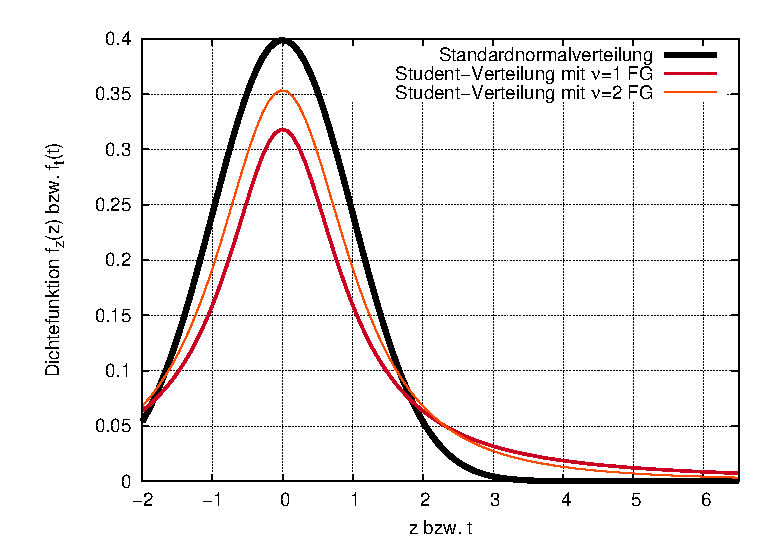
\includegraphics[width=0.5\textwidth]{figsRegr/f_gaussStudent.eps}
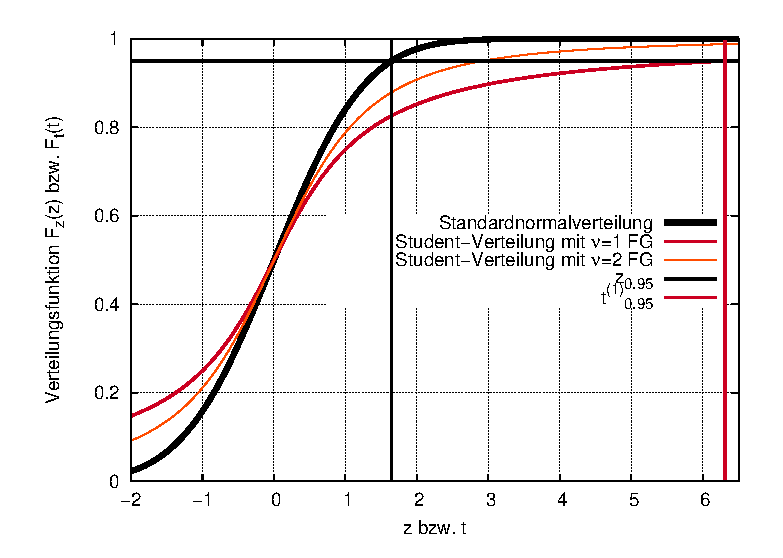
\includegraphics[width=0.5\textwidth]{figsRegr/F_gaussStudent.eps}
\caption{\label{fig:student}Dichte- und Verteilungsfunktion der
Student-t-Verteilung mit ein und zwei Freiheitsgraden und der Limes
(Standardnormalverteilung) f\"ur unendlich viele Freiheitsgrade. Bei
den Verteilungsfunktionen sind als vertikale Linien auch die Quantile
$t^{(1)}_{0.95}$ und $z_{0.95}$ der $T(1)$- bzw. der
Standardnormalverteilung eingezeichnet.
}
\end{figure}
%#############################


Gleichung~\refkl{regrT} gibt die Verteilung des Abstandes $T$ des Sch\"atzers
$\hatbeta_j$ von $\beta_j$ in Einheiten der gesch\"atzten
Standardabweichung an. 
Dreht man nun die Argumentation um, so gilt, bei G\"ultigkeit der
Gau\3-Markow-Annahmen (insbesondere Homoskedastizit\"at), dass $-T$
die bedingte Wahrscheinlicheitsverteilung des Abstandes des
wahren Wert $\beta_j$ vom Sch\"atzwert in Einheiten der gesch\"atzten
Standardabweichung bei gegebenen
Messdaten angibt. Da $T$ symmetrisch ist, ist die
\emph{Wahrscheinlichkeits-Dichte} des Abstandes des Sch\"atzers vom
wahren Wert gleich der \bfdef{Likelihood-Dichte} (bedingte
Wahrscheinlichkeitsdichte) des Abstandes des
unbekannten wahren Wertes bei gegebenem Sch\"atzer.
%#############################
\begin{figure}
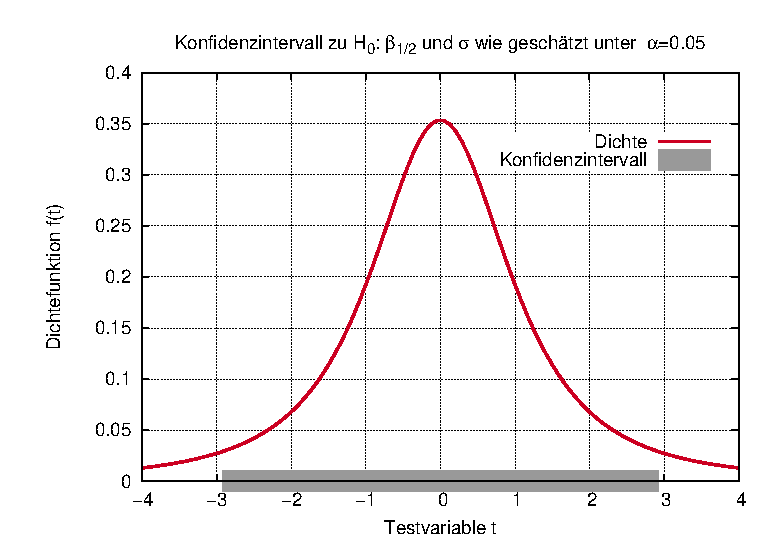
\includegraphics[width=0.5\textwidth]{figsRegr/f_student_KI.eps}
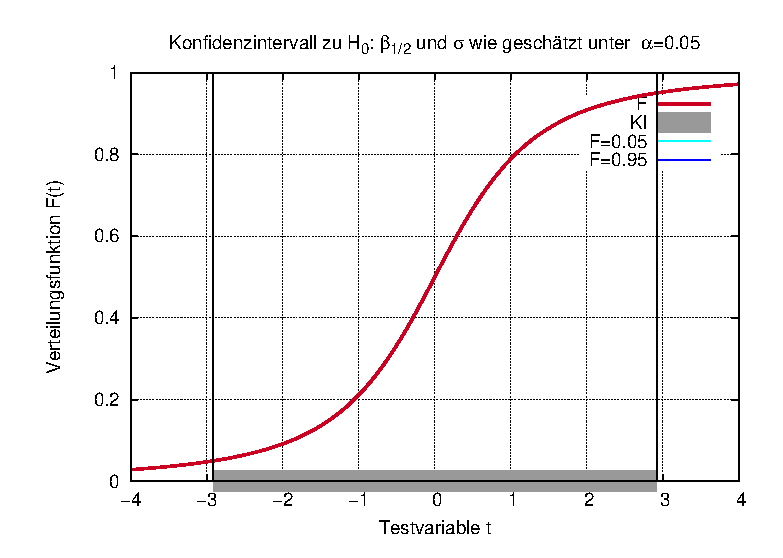
\includegraphics[width=0.5\textwidth]{figsRegr/F_student_KI.eps}
\caption{\label{fig:student-KI}Konfidenzintervall bez\"uglich des auf
die gesch\"atzte Standardabweichung bezogenen Sch\"atzwertes zu
$\alpha=\unit[5]{\%}$ Fehlerwahrscheinlichkeit f\"ur $n-J-1=2$
Freiheitsgrade. Das Intervall ist durch die Quantile
$t^{(2)}_{0.05}=-t^{(2)}_{0.95}$ 
und $t^{(2)}_{0.95}$ begrenzt.
}
\end{figure}
%#############################

Dies begr\"undet die Konfidenzintervalle: Ein
\bfdef{Konfidenzintervall} f\"ur den
wahren Parameter $\beta_j$ zur
Fehlerwahrscheinlichkeit $\alpha$ ist gleich dem um $\hatbeta_j$ symmetrischen
Intervall, in welchem der wahre Wert $\beta_j$  mit der
Wahrscheinlichkeit $1-\alpha$ liegt, also dass Intervall, was die
Fl\"ache $1-\alpha$ der Likelihoodfunktion \"uber sich vereinigt.
 Damit steht auf beiden Seiten der
Likelihood-Dichte eine Wahrscheinlichkeit (also Fl\"ache unter der
Kurve) von $\alpha/2$ f\"ur
``Ausrei\3er'' zur Verf\"ugung (Abb.~\ref{fig:test-einZweiseitig}). 
Das Konfidenzintervall wird also durch
die entsprechenden \bfdef{Quantile} der Student-t Verteilung mit
$n-J-1$ Freiheitsgraden bestimmt. Die \bfdef{Quantilsfunktion} einer
Verteilungsfunktion gibt das Argument zu einer gegebenen kumulierten 
Wahrscheinlichkeit an, ist also die \emph{Umkehrfunktion} der
Verteilungsfunktion (Abb.~\ref{fig:student}). Damit ist das
Konfidenzintervall gegeben durch (vgl. Abb.~\ref{fig:student-KI})
\maineq{KI}{
K_{\beta_j}^{(\alpha)}: \beta_j \in \left[
 \, \hatbeta_j-\Delta \hatbeta_j,  
\hatbeta_j+\Delta \hatbeta_j \,
\right], \quad
\Delta \hatbeta_j =t_{1-\alpha/2}^{(n-J-1)}\hatsig_{\hatbeta_j}.
}

%#############################
\begin{figure}
\fig{0.5\textwidth}{figsRegr/hotel_f_hatbeta1.eps}
\caption{\label{fig:KI-hotel}Likelihood-Dichte und Konfidenzintervall 
($\alpha=\unit[5]{\%}$) der
Sternenzahl-Sensitivit\"at (Anstieg der Auslastung in Prozent pro
Stern bei \emph{ceteris-paribus}-Bedingungen) im Hotelbeispiel.
}
\end{figure}
%#############################

\examplebox{Beispiel zur Begleitung: Hotel-Auslastung 
(vgl. S. \pageref{hotelbeispiel})}{
Die Konfidenzintervalle der drei Parameter zu $\alpha=\unit[5]{\%}$
betragen (vgl. Abb.~\ref{fig:KI-hotel})
\bdma
K_{\beta_0}^{(\alpha)} &=& [13.5, \, 37.5], \\
K_{\beta_1}^{(\alpha)} &=& [26.7, \, 49.7], \\
K_{\beta_2}^{(\alpha)} &=& [-1.40, \, -0.50].
\edma
Insbesondere sind beide Anstiegsparameter signifikant von null
verschieden und damit die durch die exogenen Variablen
repr\"asentierten Faktoren ``Sternezahl'' und ``Preis'' bei einer
Fehlerwahrscheinlichkeit $\alpha=\unit[5]{\%}$ beide relevant.
}

%#############################
\subsection{\label{sec:prog}Extrapolation und Prognose}
%#############################
%
Nachdem man das Modell auf korrekte Spezifikation getestet hat und
insbesondere alle nichtsignifikanten Einflussfaktoren (deren
dazugeh\"orige Anstiegsparameter nicht signifikant von null
verschieden sind) eliminiert hat, kann man (mit Sorgfalt!) durch \emph{Extrapolation}
durch das  gesch\"atzte Modell auch Aussagen in Bereichen treffen, die
nicht von den bisherigen Daten abgedeckt wurden. 
Dies wird am Beispiel der Einfachregression gezeigt. 

Mit~\refkl{VbetaEins}
erh\"alt man f\"ur das gesch\"atzte Modell
der Einfachregression die Beziehung
\bdm
\hat{Y}(x)=\hat{\beta}_0+\hat{\beta}_1 x
 = \beta_0+\beta_1x+\frac{1}{n}\sum\limits_{i=1}^n\left(
1+\frac{(x_i-\bar{x})(x-\bar{x})}{s_{xx}}\right) \epsilon_i
\edm

und damit
\be
E\left(\hat{Y}(x)\right)=\beta_0+\beta_1x.
\ee
Es sind also nicht nur die gesch\"atzten Modellparameter sondern auch
das gesamte gesch\"atzte lineare Modell  
$x$ erwartungstreu.
Die Herleitung der Varianz als Funktion der Extrapolationsvariablen
$x_1=x$ geht
analog wie die der Varianzen $V(\hat{\beta}_0)$ und $V(\hat{\beta}_1)$
in Abschnitt~\ref{sec:linStatSumme}. Man muss
nur immer beachten, dass sowohl die Messerte $x_i$ als auch $x$ als
Argument der Funktion $\hat{Y}(x)$ \textit{nichtstochastische}
Gr\"o\3en darstellen. Das Ergebnis ist die sogenannte 
``Hyperbelformel'' (vgl. Abb.~\ref{fig:hyperbel}):

\maineq{hyperbel}{
V\left(\hat{Y}(x)\right) =
\frac{\sigeps^2}{n}\left(1+\frac{(x-\bar{x})^2}{s_{xx}}\right).
}

%#######################################
\begin{figure}[t!]
\label{fig:hyperbel}
\fig{1.0\textwidth}{figsRegr/regression3d.eps}
\vspace*{-4em}

\caption{Wahrscheinlichkeitsdichte einer durch
 \protect\refkl{hyperbel} beschriebenen Normalverteilung um den 
 Erwartungswert $\beta_0+\beta_1x$ des gesch\"atzten linearen Modells.
}
\end{figure}
%#######################################


%#############################
\subsection{\label{sec:test-single}Statistische Tests eines Parameters}
%#############################

Bei den hier betrachteten \bfdef{Signifikanztests} wird eine
bestimmte Annahme, die sogenannte \bfdef{Nullhypothese} $H_0$, daraufhin
untersucht, ob sie mit den Messdaten in \"Ubereinklang sein kann oder
nicht. 

\maintext{Die Nullhypothese $H_0$ beinhaltet eine Menge von
  Parameterkombinationen des verwendeten Modells. Liegt der dem wahren
  Sachverhalt (der Grundgesamtheit) entsprechende Parametervektor
  in dieser Menge, sagt man, $H_0$ sei erf\"ullt.}

\emph{Hinweis:} Sind die Gau\3-Markow-Annahmen, insbesondere die
Homogenit\"atsannahme, erf\"ullt, gibt es einen eindeutigen und
unver\"anderlichen wahren Wert des Parametervektors in der Grundgesamtheit. $H_0$ ist also
entweder objektiv erf\"ullt oder nicht.

\emph{Hinweis 2:}  Die Nullhypothese $H_0$ kann im Prinzip beliebig
formuliert werden. Man sollte sie so w\"ahlen, dass deren
\emph{Ablehnung} einer relevanten Aussage entspricht, denn
es gilt:

\maintext{Eine signifikante Aussage gewinnt man bei Signifikanztests
nur, wenn man die  Nullhypothese $H_0$ verwerfen kann. Ist dies
bei einer gewissen Fehlerwahrscheinlichkeit $\alpha$ 
nicht m\"oglich, hei\3t das nicht, dass $H_0$ ``angenommen'' wird,
sondern dass keine statistische Aussage m\"oglich ist!}

Diese Aussage wird dadurch klar, wenn man die in
Abb.~\ref{fig:fehlerErsterZweiterArt} dargestellten 
Konsequenzen einer Testentscheidung n\"aher betrachtet. Die Zeilen
stellen dabei den objektiven Sachverhalt dar: $H_0$ ist entweder wahr
oder falsch (aufgrund der Homogenit\"atsannahme ist diese
Unterscheidung, wie gesagt, immer eindeutig). Die Spalten stellen die
Testentscheidung dar: $H_0$ annehmen oder nicht. Damit sind vier
F\"alle m\"oglich:

%#############################
\begin{figure}
\fig{0.5\textwidth}{figsRegr/fehlerErsterZweiterArt.eps}
\caption{\label{fig:fehlerErsterZweiterArt}Definition der Fehler
erster und zweiter Art bei Signifikanztests.
}
\end{figure}
%#############################
\bi
\item $H_0$ trifft zu und der Test wird nicht abgelehnt: Richtige Schlussfolgerung
\item $H_0$ trifft nicht zu und der Test wird abgelehnt: Richtige Schlussfolgerung
\item $H_0$ trifft zu und der Test wird abgelehnt. Dann hat man einen
\bfdef{Fehler erster Art} bzw. einen \bfdef{$\alpha$-Fehler}
begangen. Dieser l\"asst sich mit der Fehlerwahrscheinlichkeit
$\alpha$ (z.B. $\alpha=\unit[5]{\%}$) kontrollieren.
\item $H_0$ trifft nicht zu und der Test wird nicht abgelehnt. 
Dann hat man einen
\bfdef{Fehler zweiter Art} bzw. einen \bfdef{$\beta$-Fehler}
begangen. Dieser l\"asst sich im Allgemeinen \emph{nicht}
kontrollieren. Dessen  Wahrscheinlichkeit kann durchaus $1-\alpha$
erreichen, also z.B. \unit[95]{\%},
vgl. Abschnitt~\ref{sec:fehlerZweiterArt}.
 Daher kommt die Regel, dass man
Nullhypothesen nur ablehnen, nicht aber ``annehmen'' kann!
\ei

Die Vorgehensweise bei Signifikanztests verl\"auft immer nach
demselben Schema:
\benum
\item \textbf{Formulierung der Nullhypothese $H_0$:} Dies kann erfolgen als 
\bi
\item \bfdef{Punkthypothese bzw. zweiseitiger Test:} $\beta_j=\beta_{j0}$, z.B. $\beta_j=0$, und als
\item \bfdef{Intervallhypothese bzw. einseitiger Test:} 
$\beta_j<\beta_{j0}$, $\beta_j \le \beta_{j0}$, 
$\beta_j>\beta_{j0}$, $\beta_j \ge \beta_{j0}$,
\item \bfdef{gekoppelte Nullhypothesen}, z.B. $\beta_1/\beta_2<1$. 
\ei
Die Nullhypothese wird in Hinblick auf die gew\"unschte Aussage
getroffen.  Da man $H_0$ nicht ablehnen kann, behauptet man in $H_0$
immer das Gegenteil der zu untersuchenden Aussage, so dass man bei
Ablehnung die Aussage selbst signifikant ``best\"atigt'' hat. Will man
beispielsweise die Klimaerw\"armung nachweisen, stellt man sich auf
den Standpunkt eines Klimaskeptikers: Die Nullhypothese lautet also,
dass die globale Durchschnittstemperatur sinkt oder stagniert bzw. der
entsprechende Anstiegparameter nichtpositiv ist. Dies
versucht man dann zu widerlegen.

\examplebox{Beispiel zur Begleitung: Hotel-Auslastung 
(vgl. S. \pageref{hotelbeispiel})}{
\label{hotelbeispiel-H0}
Das betrachtete Modell lautete
$y=\beta_0+\beta_1x_1+\beta_2x_2+\epsilon$. Hierbei ist $x_1$ der
Qualit\"atsindikator ``Sternzahl'' und $x_2$ der \"Ubernachtungspreis in
Eurpo pro Nacht. sinnvolle Nullhypothesen sind u.a.:
\bi
\item $H_{01}: \beta_1=0$: ``Die Qualit\"at ist egal. Wenn \"uberhaupt, dann
  entscheidet nur der Preis''.
\item $H_{02}: \beta_1 \le 0$: ``Ich liebe schlechte
  Hotels''. Nat\"urlich versucht man, diese Hypothese zu widerlegen,
  um damit signifikant nachzuweisen, dass die Qualit\"at eben
  \emph{nicht} egal ist.
\item $H_{03}: \beta_2=0$: ``Der Preis ist egal''.
\item $H_{04}: \beta_2<=-1$:``Jeder Euro Preiserh\"ohung vergrault so viele
  G\"aste, dass die Auslastung um mindestens \unit[1]{\%}
  sinkt''. Auch dies versucht man nat\"urlich zu widerlegen (``der
  Schwund betr\"agt h\"ochstens \unit[1]{\%} pro Euro Preisaufschlag''),
  was dem Hotelmanager als Entscheidungshilfe f\"ur die k\"unftige
  Preisgestaltung dienen kann.
\item $H_{05}: \beta_1+30\beta_2\le 0$: ``Ein Stern mehr ist mir
  h\"ochstens 30 Euro pro Nacht wert''. Eine Widerlegung dieser
  Aussage beinhaltet, dass nach einer Renovierung, z.B. von einem
  Drei- in ein Viersternehotel, pro Nacht 30 Euro mehr verlangt werden
  kann, ohne einen G\"aster\"uckgang bef\"urchten zu m\"ussen. 
\ei
}


\item \textbf{Formulierung der Testgr\"o\3e (``Test-Statistik''):}
Im realistischen Fall unbekannter Residualvarianz verwendet man bei
Tests der Regressionsparameter direkt
den Abstand $T$ vom Rand des Parameterbereich, in welchem $H_0$ gilt
(Rand der $H_0$-Menge) und zwar
\emph{in Einheiten der gesch\"atzten 
Standardabweichung.}  Dabei rechnet man immer unter der Voraussetzung,
dass $H_0$ tats\"achlich \emph{grenzwertig} zutrifft:
\bi
\item 
Bei einer Punkthypothese ist dies eindeutig: Der wahren Wert $\beta_j$
wird gleich dem 
Nullhypothesen-Wert $\beta_{j0}$ gesetzt.
\item Umfasst die
Nullhypothesenmenge ein ganzes Intervall (Intervallhypothese), wird der 
\emph{Worst Case} angenommen, also der Wert aus der
Nullhypothesenmenge, bei dem
ein Fehler erster Art die h\"ochste Wahrscheinlichkeit hat. Dieser
liegt immer auf der Grenze des $H_0$-Intervalls bzw. am Rande des
Parameterbereichs, in welchem $H_0$ zutrifft.
\item Bei einer gekoppelten Nullhypothese wird eine
  Parameterkombination ein\-ge\-f\"uhrt, bez\"uglich derer der Test einer
  einfachen Punkt- oder Intervallhypothese ent\-spricht,
  z.B. $\gamma=\beta_1+30\beta_2$ f\"ur die Nullhypothesen
  $\beta_1<-30\beta_2$, $\beta_1>-30\beta_2$ oder $\beta_1=-30\beta_2$.
\ei
Daraus folgt: 

\maintext{Unabh\"angig von der Art der Nullhypothese ($=, \ge, >, \le,
<$) ist die Testvariable $T$ (``Test-Statistik'') des $t$-Tests immer der
gerichtete Abstand des Parametersch\"atzers vom Rand der Nullhypothese
in Einheiten der gesch\"atzten Standardabweichung: 
\be
\label{test-T}
T_{\beta_j}= \frac{\hat{\beta}_j-\beta_{j0}}{\sqrt{\hat{V}(\hat{\beta}_j)}}
:= \frac{\hat{\beta}_j-\beta_{j0}}{\hatsig_{\hatbeta_j}}.
\ee
\emph{Falls} $H_0$ grenzwertig zutrifft, ist diese Testvariable Student-t verteilt mit $n-1-J$ Freiheitsgraden
(Zahl der Datens\"atze abz\"uglich Zahl der zu sch\"atzenden
Parameter):
\be
T_{\beta_j} \sim T(n-J-1).
\ee
\vspace{-1.5em}
}

\item \textbf{Berechnen einer Instanz (Realisierung) $t_{\beta_j}$ der
Testvariablen} aus der Stichprobe.

%################
\examplebox{Hotelbeispiel}{
Die Testgr\"o\3e f\"ur die Nullhypothesen $H_{01}$ und $H_{02}$
und die aus den Daten berechnete Instanz lautet:
\bdm
T_1=T_2=\frac{\hat{\beta}_1}{\sqrt{\hat{V}_{11}}}\sim T(9)
\edm
und die Realisierung
\bdm
t_1=t_2=\frac{38.2}{\sqrt{26.0}}=7.49.
\edm
F\"ur $H_{03}$ ergibt sich,
\bdm
T_3=\frac{\hat{\beta}_2}{\sqrt{\hat{V}_{22}}}\sim T(9), \quad
t_3=\frac{-0.952}{\sqrt{0.0397}}=-4.78
\edm
und f\"ur $H_{04}$ 
\bdm
T_4=\frac{\hat{\beta}_2+1}{\sqrt{\hat{V}_{22}}}\sim T(9), \quad
t_4=\frac{0.048}{\sqrt{0.0397}}=0.237.
\edm
}

\examplebox{}{
Die f\"unfte kombinierte Nullhypothese
(vgl. Abschnitt~\ref{sec:kombi}) kann man umformulieren zu
\bdm
\gamma=\beta_1+30\beta_2<0
\edm
und damit
\bdm
T_5=\frac{\hat{\gamma}}{\sqrt{\hat{V}(\hat{\gamma})}}\sim T(9).
\edm
Mit
\bdma
\hat{\gamma} &=& \hatbeta_1+30\hatbeta_2=9.63, \\
\hat{V}(\hat{\gamma}) &=& \hat{V}_{11}+60\hat{V}_{12}+900 \hat{V}_{22}
=5.27
\edma
ergibt dies die Realisierung
\bdm
t_5=\frac{9.63}{\sqrt{5.27}}=4.20
\edm
}
%################



\item \textbf{Auswertung des Tests}
Die Testaussage ``$H_0$ kann abgelehnt werden'' h\"angt wieder von der
Nullhypothese ab:
\bi
\item Bei \emph{zweiseitigen Tests}  teilt man, wie bei den Konfidenzintervallen,
die Fehlerwahrscheinlichkeit auf beiden Seiten gleichm\"a\3ig auf
(vgl. Abb.~\ref{fig:test-einZweiseitig}). Die Nullhypothese 
$\beta_j=\beta_{j0}$ kann bei einer Fehlerwahrscheinlichkeit von
$\alpha$  abgelehnt werden, falls
die Realisierung der Teststatistik der Bedingung
\be
\label{testbsymm}
|t_{\beta_j}| > t_{1-\alpha/2}^{(n-J-1)}
\ee
gen\"ugt. Auf der rechten Seite steht dabei das (tabellierte) Quantil
der $T$-Verteilung mit $n-1-J$ Freiheitsgraden. 
Mit der Nullhypothese $\beta_{j0}=0$ findet dieser Test 
vor allem Anwendung, wenn man 
Einflussfaktoren (exogene Variable) auf Signifikanz oder speziell
Zeitreihen auf das 
Vorhandensein eines Trends pr\"ufen will.

\item \emph{Einseitige Tests}: Hier kann man die volle
Fehlerwahrscheinlichkeit auf jeweils eine Seite der Test-Statistik $T$
h\"aufen: 
\bi
\item $H_0:\beta_j<\beta_{j0}$ und  $H_0:\beta_j \le \beta_{j0}$ ist
bei einer Fehlerwahrscheinlichkeit von $\alpha$ ablehnbar, falls
\be
\label{testasymm-gt}
t_{\beta_j} > t_{1-\alpha}^{(n-J-1)}.
\ee
\item $H_0:\beta_j>\beta_{j0}$ und  $H_0:\beta_j \ge \beta_{j0}$ ist
bei einer Fehlerwahrscheinlichkeit von $\alpha$ ablehnbar, falls
\be
\label{testasymm-lt}
t_{\beta_j} < t_{\alpha}^{(n-J-1)}=-t_{1-\alpha}^{(n-J-1)}.
\ee
\ei
\ei
\eenum

%################
\examplebox{Hotelbeispiel}{
Im folgenden wird versucht, die obigen Nullhypothesen bei
$\alpha=\unit[5]{\%}$ Fehlerwahrscheinlichkeit zu widerlegen.
\bdm
\begin{array}{lll}
H_{01}: \beta_1=0, & |t_1|=7.49 >t^{(9)}_{0.975}=2.26 & \Rightarrow
\ \text{ja, also $H_{01}$ widerlegt!}\\
H_{02}: \beta_1<0, & t_2=7.49 >t^{(9)}_{0.95}=1.83 & \Rightarrow
\ \text{ja, also $H_{02}$ widerlegt!}\\
H_{03}: \beta_2=0, & |t_3|=+4.78 >t^{(9)}_{0.975}=2.26 & \Rightarrow
\ \text{ja, also $H_{03}$ widerlegt!}\\
H_{04}: \beta_2<-1,  &t_4=0.24>t^{(9)}_{0.95}=1.83 & \Rightarrow
\ \text{nein, $H_{04}$ nicht widerlegbar!}\\
H_{05}: \gamma<0, & t_5=4.20>t^{(9)}_{0.95}=1.83 & \Rightarrow
\ \text{ja, also $H_{05}$ widerlegt!}
\end{array}
\edm
}
%################



%
Zweiseitige Tests bzw. Punkt-Nullhypothesen werden genau dann
abgelehnt, wenn die Nullhypothese nicht im Konfidenzintervall (zu
gleicher Fehlerwahrscheinlichkeit) liegt.

%#############################
\begin{figure}
\fig{0.6\textwidth}{figsRegr/annahmeAblehn_einZweiseit.eps}
\caption{\label{fig:test-einZweiseitig}Annahme- und Ablehnungsbereiche
bei (a) einseitigen Tests (Tests einer Punkt-Hypothese), (b,c)
zweiseitigen  Tests (Intervallhypothese). 
}
\end{figure}
%#############################


%#######################################
\subsection{\label{sec:pWert}p-Werte} 
%#######################################
Eigentlich ist das Vorgehen, einen Test bei einer vorher festgelegten
Fehlerwahrscheinlichkeit abzulehnen zu versuchen,
umst\"andlich und man verschenkt ggf. einiges an Sch\"arfe in den
Aussagen. Beispielsweise k\"onnte eine Nullhypothese, welche man bei
$\alpha=\unit[5]{\%}$ ablehnen konnte, auch bei \unit[0.1]{\%}
ablehnbar sein und damit die damit verbundene Aussage nicht nur
signifikant, sondern ``hochsignifikant''. 
Interessant ist deshalb eigentlich der \emph{Grenzwert} der
Fehlerwahrscheinlichkeit, bei dem man einen Test \emph{gerade noch}
ablehnen kann:

\maintext{Der \bfdef{$p$-Wert} (engl.: \textit{p-value}) ist die
  Grenz-Fehlerwahrscheinlichkeit, bei der $H_0$ gerade noch abgelehnt
  werden kann:
  \be
  \label{def-p}
p =\min\left(\alpha | \
 \text{$H_0$ ist ablehnbar bei Fehlerwahrscheinlichkeit
   $\alpha$}\right). 
\ee
\vspace{-2em}
}
Eine allgemeinere Definition von $p$ werden wir in
Kap.~\ref{sec:bayes} kennenlernen:
\maintext{Der $p$-Wert zu einer Beobachtung $b$ gibt die
  Wahrscheinlichkeit daf\"ur an, die Beobachtung oder einen ``extremeren''
  Wert zu erhalten, falls die Nullhypothese \emph{grenzwertig
    zutrifft}.}
%
Nach~\refkl{def-p} ergibt sich $p$ aus den Test-Entscheidungsgleichungen,
  indem man $\alpha$ durch $p$ und die Ungleichheitszeichen durch
  Gleichheitszeichen ersetzt, z.B.
beim Test auf ``kleiner'' oder ``kleiner gleich'':
$t_{\beta_j} > t_{1-\alpha}^{(n-J-1)} \to  t_{\beta_j} = t_{1-p}^{(n-J-1)}$. 
Um dies nach dem $p$-Wert aufzul\"osen, nutzt man aus, 
dass die Quantile
nichts anderes als die Umkehrfunktion der entsprechenden (kumulierten)
Verteilungsfunktion darstellen, beispielsweise bei den
Student-t und Standardnormalverteilungen:
\maineq{quantileUmkehr}{
F_T(t_{\alpha})=\alpha, \quad
\Phi(z_{\alpha})=\alpha
}
mit $F_T(t)$ der Verteilungsfunktion der jeweiligen
Student-t-Verteilung mit $m$ Freiheitsgraden, $t_{\alpha}$ das
jeweilige Quantil (der Index $m$ f\"ur die Freiheitsgrade wurde der
\"Uber\-sicht\-lich\-keit halber weggelassen), $\Phi(z)$ die
Verteilungsfunktion der Standardnormalverteilung und $z_{\alpha}$ die
Quantilsfunktion der Standardnormalverteilung. Konkret f\"uhrt dies
auf folgende Ausdr\"ucke f\"ur die $p$-Werte:  
\bi
\item Zweiseitige Tests bzw. Punkthypothesen bei
  gegebener Realisierung $t$ der Test-Statistik $T \sim T(n-1-J)$:
\bdma
p 
&=&\min\left(\alpha | \ \text{so dass} \ |t|\ge t_{1-\alpha/2}\right)\\
 \Leftrightarrow  |t| &=& t_{1-p/2}\\
  F_T(|t|) &=& 1-\frac{p}{2}, 
\edma
also
\be
p = 2 \left(1-F_T(|t|)\right).
\ee

\item Bei  einseitigen Tests auf $>$ bzw. $\ge$ gilt analog
\be
p=P(T<t)=F_T(t)
\ee
\item Bei  einseitigen Tests auf $<$ bzw. $\le$ gilt
\be
p=P(T>t)=1-F_T(t)
\ee
\ei

Die durch den $p$-Wert erhaltene Aussage teilt man h\"aufig in drei
Klassen ein:
\vspace{1em}

\maintext{
\bi
\item $p > \unit[5]{\%}$: Keine signifikante Aussage, da $H_0$ nicht
abgelehnt werden kann
\item $\unit[1]{\%} \le p < \unit[5]{\%}$: Durch die Ablehnung von
$H_0$ erh\"alt man eine \emph{signifikante} Aussage. Ist dieses
Signifikanzniveau bei einem Test eines Parameters  auf den Wert 0
erreicht, so bekommt der Zahlenwert des Parameters per Konvention der
meisten Statistikprogramme einen Stern, z.B. $\beta_1=2.1^*$
\item $\unit[0.1]{\%} \le p < \unit[1]{\%}$: Durch die Ablehnung von
$H_0$ erh\"alt man eine \emph{sehr signifikante} Aussage. Ist ein
Parameter auf diesem
Signifikanzniveau von null verschieden, so bekommt der Zahlenwert zwei
Sterne, z.B. $\beta_2=-3.14^{**}$ 
\item $p < \unit[0.1]{\%}$: Durch die Ablehnung von
$H_0$ erh\"alt man eine \emph{hochsignifikante} Aussage. Ist ein
Parameter auf diesem
Signifikanzniveau von null verschieden, so bekommt der Zahlenwert drei
Sterne, z.B. $\beta_3=42^{***}$ 
\ei
}


\examplebox{Beispiel zur Begleitung: Hotel-Auslastung 
(vgl. S. \pageref{hotelbeispiel})}{
Die $p$-Werte der f\"unf Nullhypothesen auf
S.~\pageref{hotelbeispiel-H0} errchnen sich zu
\bdm
\begin{array}{lll}
H_{01}: \beta_1=0, & |t_1|=7.49 & p= 2(1-F_T^{(9)})(|t_1|)=3.7\times 10^{-5}***\\
H_{02}: \beta_1<0, & t_2=7.49 & p= 1-F_T^{(9)}(t_2)=1.9\times 10^{-5}***\\
H_{03}: \beta_2=0, & |t_3|=+4.78 & p=2(1-F_T^{(9)})(|t_3|)=\unit[0.10]{\%}** \\
H_{04}: \beta_2<-1,  &t_4=0.24 & p=1-F_T^{(9)}(t_4)=\unit[40]{\%} \\
H_{05}: \gamma<0, & t_5=4.20 & p= 1-F_T^{(9)}(t_5)=\unit[0.12]{\%}** \\
\end{array}
\edm

Die kritischen Fehlerwahrscheinlichkeiten sind also meist sehr
signifikant mit $p$-Werten h\"aufig kleiner als \unit[1]{\%}. 
 Ein Test von beispielsweise $H_{01}$ bei
$\alpha=\unit[5]{\%}$ ergibt 
mit $t_{0.975}^{(9)}=2.4$ eine Ablehnung, in \"Ubereinstimmung mit den
Konfidenzintervallen,  aber man verschenkt die
Aussage, dass dies nicht nur bei $\alpha=\unit[5]{\%}$ gilt, sondern
hinunter bis zu $\alpha=p=0.0037\%$.
}
%################



%#######################################
\subsection{\label{sec:fehlerZweiterArt}G\"utefunktion und Fehler
zweiter Art} 
%#######################################
Hier wird kurz erl\"autert, warum man den Fehler zweiter Art nicht
bzw. nicht gleichzeitig mit dem Fehler erster Art kontrollieren
kann. Dazu definieren wir zun\"achst die G\"utefunktion:

\maintext{Die \bfdef{G\"utefunktion} ist definiert als die 
Ablehnwahrscheinlichkeit des Tests in Abh\"angigkeit des \emph{wahren}
Parameterwertes $\beta_j$.
}
\vspace{1em}

\noindent
Wieder unterscheiden wir zwischen zweiseitigen und einseitigen Tests:

\subsubsection*{Zweiseitige Tests}
Zun\"achst ist klar, dass bei stetigen Parameterwerten (die in der
Regressionsrechnung immer Voraussetzung sind!) eine Punkthypothese  
$\beta_j=\beta_{j0}$ 
eigentlich \emph{nie} erf\"ullt sein kann, da die Menge von $H_0$ das ``Ma\3
null'' (bzw. das $H_0$ entsprechende Intervall die L\"ange null)
aufweist. Damit ist die Wahrscheinlichkeit eines Fehlers
 zweiter Art direkt durch eins
minus der Ablehnwahrscheinlichkeit des Tests gegeben. 

Zum Berechnen der G\"utefunktion f\"ur $\beta_j \neq \beta_{j0}$ muss man sich klarmachen, 
dass dann die Test-Variable
$(\hatbeta_j-\beta_{j0})/\hatsig_{\hatbeta_j}$ \emph{nicht} mehr
Student-t-verteilt ist, sondern vielmehr die Variable
\bdm
T=\frac{\hatbeta_j-\beta_j}{\hatsig_{\hatbeta_j}}
 = \frac{\hatbeta_j-\beta_{j0}+\beta_{j0}-\beta_j}{\hatsig_{\hatbeta_j}}
 = \frac{\hatbeta_j-\beta_{j0}}{\hatsig_{\hatbeta_j}}-\Delta T.
\edm
Im letzten Ausdruck ist der erste Summand die beim Test verwendete
Testvariable und
\bdm
\Delta T=\frac{\beta_j - \beta_{j0}}{\hatsig_{\hatbeta_j}}
\edm
der Abstand des wahren Wertes vom Grenzwert $\beta_{j0}$ in Einheiten
der gesch\"atzten Standardabweichung.
Gem\"a\3 Punkt 4 (Entscheidung) des Test-Schemas ist die
G\"utefunktion $G\sup{\,eq}(\Delta T)$ , definiert als die 
\emph{Ablehnwahrscheinlichkeit} der Gleichheitsbedingung (Superskript
``eq'' f\"ur ``equality'') bei einer formalen
``Fehlerwahrscheinlichkeit'' $\alpha$ in Abh\"angigkeit der Abweichung
$\Delta T$ (``G\"utefunktion'') gegeben durch
\bdma
G\sup{\,eq}(\Delta T) 
 &=& P\left(\left|\frac{\hatbeta_j-\beta_{j0}}{\hatsig_{\hatbeta_j}}\right|
      > t_{1-\alpha/2}\right) \\
&=& P(|T+\Delta T| > t_{1-\alpha/2}) \\
&=& P(T+\Delta T > t_{1-\alpha/2}) + P(T+\Delta T <-t_{1-\alpha/2})\\
&=& 1-P(T+\Delta T \le t_{1-\alpha/2})+P(T+\Delta T <-t_{1-\alpha/2})\\
\edma
und mit der (kumulierten) Verteilungsfunktion $F_T(t)$ der
Student-t-Verteilung unter Verwendung von $F_T(-t)=1-F_T(t)$
\bea
\label{GuetefunEq}
G\sup{\,eq}(\Delta T) 
&=& 1-F_T(t_{1-\alpha/2}-\Delta T) + F_T(-t_{1-\alpha/2}-\Delta T) \nonumber \\
&=& 2-F_T(t_{1-\alpha/2}-\Delta T) - F_T(t_{1-\alpha/2}+\Delta T) \nonumber 
\eea
\emph{Probe:}
\bdma
 G\sup{\,eq}(0)=2-F_T(t_{1-\alpha/2})-F_T(t_{1-\alpha/2})=2-2+2\alpha/2 = \alpha \ \OKeps \\
 \lim\limits_{\Delta T \to -\infty}G\sup{\,eq}(\Delta T)=2-F_T(\infty)-F_T(-\infty)=1 \ \OKeps \\
 \lim\limits_{\Delta T \to +\infty}G\sup{\,eq}(\Delta T)=2-F_T(-\infty)-F_T(\infty)=1 \ \OKeps \\
\edma

%#############################
\begin{figure}
\fig{0.5\textwidth}{figsRegr/fehler12art_eqStudent_2FG.eps}
\caption{\label{fig:fehler12art-eq}G\"utefunktion und Fehler
erster und zweiter Art bei zweiseitigen Tests (Punkthypothesen) in
Abh\"angigkeit des skalierten Abstandes $\Delta
t=(beta_j-\beta_{0j})/\hatsig_{\hatbeta_j}$ des wahren Parameterwertes von
der Nullhypothese. Beispiel f\"ur $\alpha=\unit[10]{\%}$ und $n-J-1=2$
Freiheitsgrade.
}
\end{figure}
%#############################

%#############################
\begin{figure}
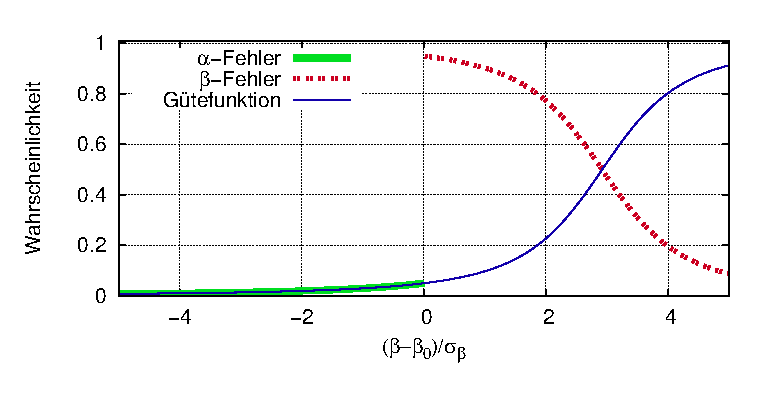
\includegraphics[width=0.5\textwidth]{figsRegr/fehler12art_leStudent_2FG.eps}
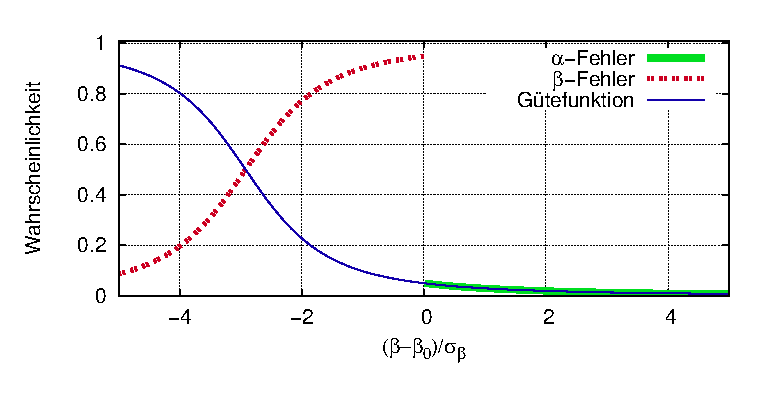
\includegraphics[width=0.5\textwidth]{figsRegr/fehler12art_geStudent_2FG.eps}
\caption{\label{fig:fehler12art-neq}G\"utefunktion und Fehler
erster und zweiter Art bei einseitigen Tests auf $<, \le$ (links) und
$>, \ge$ (rechts) in
Abh\"angigkeit des skalierten Abstandes $\Delta
t=(\beta_j-\beta_{0j})/\hatsig_{\hatbeta_j}$ des wahren Parameterwertes vom
Grenzwert der Nullhypothese. Beispiele
 f\"ur $\alpha=\unit[10]{\%}$ und $n-J-1=2$ Freiheitsgrade.
}
\end{figure}
%#############################

\noindent
Abbildung~\ref{fig:fehler12art-eq} zeigt das Ergebnis: Die
Wahrscheinlichkeit eines Fehlers
zweiterArt kann bis zu $1-\alpha$ betragen, man wei\3 aber noch nicht
mal den konkreten Wert dieser bedingten Wahrscheinlichkeit, da die
Bedingung (=der wahre Wert $\beta_j$) nicht bekannt ist. \emph{in jedem
Fall ist aber die Wahrscheinlichkeit eines Fehlers erster Art
h\"ochstens gleich $\alpha$.}

\subsubsection*{Einseitige Tests}
Die Berechnung der G\"utefunktion f\"ur einseitige Tests geht analog:

\textbf{Test auf ``$>$'' oder ``$\ge$''}:
\bdma
G^{\ge}(\Delta T)
 &=& P\left(\frac{\hatbeta_j-\beta_{j0}}{\hatsig_{\hatbeta_j}}
    <t_{\alpha}\right)\\
 &=& P(T+\Delta T<t_{\alpha}) \\
 &=& P(T<-\Delta T+t_{\alpha}) \\
\edma
und damit
\be
\label{GuetefunGe}
G^{\ge}(\Delta T)=F_T(t_{\alpha}-\Delta T)
\ee
\emph{Probe:}
\bdma
 G^{\ge}(0)=F_T(t_{\alpha}) = \alpha \ \OKeps \\
 \lim\limits_{\Delta T \to -\infty}G^{\ge}(\Delta T)=F_T(\infty)=1 \ \OKeps \\
 \lim\limits_{\Delta T \to \infty}G^{\ge}(\Delta T)=F_T(-\infty)=0 \ \OKeps \, .
\edma

\textbf{Test auf ``$<$'' oder ``$\le$''}:
\bdma
G^{\le}(\Delta T)
 &=& P\left(\frac{\hatbeta_j-\beta_{j0}}{\hatsig_{\hatbeta_j}}
    >t_{1-\alpha}\right)\\
 &=& P(T+\Delta T>t_{1-\alpha}) \\
 &=& P(T>-\Delta T+t_{1-\alpha}) \\
 &=& 1-P(T<-\Delta T+t_{1-\alpha})
\edma
und damit
\be
\label{GuetefunLe}
G^{\le}(\Delta T)=F_T(\Delta T-t_{1-\alpha})
\ee
\emph{Probe:}
\bdma
 G^{\le}(0) &=& F_T(-t_{1-\alpha})=1-F_T(t_{1-\alpha})=1-(1-\alpha)=\alpha \ \OKeps,\\
 \lim\limits_{\Delta T \to -\infty}G^{\le}(\Delta T) &=& F_T(-\infty)=0 \ \OKeps, \\
\lim\limits_{\Delta T \to \infty}G^{\le}(\Delta T) &=& F_T(\infty)=1 \ \OKeps
\edma


Abbildung~\ref{fig:fehler12art-neq} zeigt, dass auch hier die
Wahrscheinlichkeit eines Fehlers
zweiter Art bis zu $1-\alpha=\unit[90]{\%}$ betragen kann, w\"ahrend
die Wahrscheinlichkeit eines Fehlers erster Art h\"ochstens gleich $\alpha$,
u.U. aber auch wesentlich kleiner ist.

%#############################
%\examplebox{Hotelbeispiel:}{
\begin{figure}
\fig{1.0\textwidth}{figsRegr/hotel_f2_hatbeta1_hatbeta2.eps}
\caption{\label{fig:hotel-konfidenzregion}Zweidimensionale
Konfidenzregionen des Hotelbeispiels f\"ur die beiden
Anstiegsparameter $\beta_1$ und $\beta_2$. Kontourplot: 
Auf den maximalen Wert 1 normierte 
Likelihood-Dichte der verbundenen Wahrscheinlichkeiten, dass
 $\beta_1$ und $\beta_2$ die jeweiligen Werte annehmen. Gr\"unes
Rechteck: Konfidenzregion als kartesisches Produkt zweier unverbundener
Konfidenzintervalle (zu $\alpha=\unit[5]{\%}$). Punkt-Nullhypothesen, welche
Punkten innerhalb des Rechtecks entsprechen, werden von keinem der
beiden 
einfachen $T$-Tests abgelehnt. Blaue Ellipse:
Verbundene Konfidenzregion, innerhalb der sich beide Anstiegsparameter
simultan mit $1-\alpha=\unit[95]{\%}$ Wahrscheinlichkeit
aufhalten. Nullhypothesen au\3erhalb der blauen Ellipse aber innerhalb
des Rechtecks werden vom verbundenen $F$-Test, nicht aber von den
beiden $T$-Tests abgelehnt.
Hellblaue parallele Linien: Konfidenzintervalle (=Abstand der
jeweiligen Linien)  der Linearkombinationen $\gamma_1=\beta_2+c\beta_1$ und
$\gamma_2=\beta_2-c\beta_1$ mit $c=(V_{22}/V_{11})^{1/2}$. Auch das durch
diese Linien aufgespannte Paralellogramm ist eine Konfidenzregion (mit
einer kleineren Fl\"ache als das Rechteck.) Die
beiden schwarzen Symbole geben zwei verbundene Punkt-Nullhypothesen an, 
welche in Abschnitt~\ref{sec:test-multi} betrachtet werden: $H_{01}$
(gef\"ullter Kreis) und $H_{02}$ (Dreieck). Schlie\3lich kennzeichnet
die schwarze gerade die obere Grenze der kombinierten
Intervall-Nullhypothese $\gamma=\beta_1+30\beta_2 < 0$.
}
\end{figure}

%#############################


%#############################
\subsection{\label{sec:KI-multi}Konfidenzregionen von
Parameterkombinationen} 
%#############################
Aufgrund der Korrelationen bei den Abweichungen der
Parametersch\"atzer von den tat\-s\"ach\-lichen Werten
(vgl. Abb.~\ref{fig:hotel-konfidenzregion}) gibt es bei mehr als einem
zu sch\"atzenden Parameter gegen\"uber der naheliegenden seriellen
Analyse jedes einzelnen Parameters nichttriviale weitere
Sch\"atz-M\"oglichkeiten, insbesondere Konfidenzintervalle von
Parameterkombinationen und mehrdimensionale Konfidenzregionen.

%#############################
\subsubsection{Konfidenzintervalle von Parameterkombinationen}
%#############################

Das gew\"ohnliche, bisher betrachtete Konfidenzintervall eines
Parameters gilt f\"ur beliebige Werte der anderen Parameter. Im Raum
aller Parameter stellen die Begrenzungen der Intervalle daher Geraden
(2 Parameter), Ebenen (3 Parameter) oder Hyperebenen ($>3$ Parameter)
dar. In Abb. ~\ref{fig:hotel-konfidenzregion} sind f\"ur das
``Hotelbeispiel'' die
Begrenzungen der Konfidenzintervalle von $\beta_1$ und $\beta_2$
als gr\"une senkrechte bzw. waagerechte Geraden im von $\beta_1$ und
$\beta_2$ aufgespannten Unterraum des Raums aller Parameter 
$(\beta_0,\beta_1,\beta_2)$ gezeichnet. Die
Likelihood-Dichte~\refkl{betaDensity} legt f\"ur dieses Beispiel nahe,
dass \emph{Linearkombinationen} der Ansteigsparameter, z.B. durch die
schr\"agen blauen Geraden charakterisiert,  m\"oglicherweise
sehr viel kleinere Konfidenzintervalle aufweisen und damit sch\"arfere
Aussagen erlauben k\"onnten. 
Eine allgemeine Linearkombination hat die Form
\be
\gamma=\sum_jc_j\beta_j
\ee
mit dem Sch\"atzer
\be
\hat{\gamma}=\sum_jc_j\hatbeta_j.
\ee
%
Mit Hilfe elementarer Statistik-Regeln ist es ein Leichtes,
Erwartungswert, Varianz und Verteilung von $\hat{\gamma}$ zu bestimmen:
\bi
\item \textbf{Erwartungswert:}
\bdm
E(\hat{\gamma})=\sum_jc_jE(\hatbeta_j)=\sum_j c_j \beta_j.
\edm

\item \textbf{Varianz:}
\be
\label{vargamma}
V(\hat{\gamma})=\sum_j\sum_k c_jc_k\,\text{Cov}\, (\hatbeta_j, \hatbeta_k)
 = \sum_j\sum_k c_jc_kV_{jk}
\ee

\item \textbf{Verteilung:}
Eine Linearkombination von (korrelierten oder nicht korrelierten)
gau\3verteilten Zufallsvariablen ist wieder gau\3verteilt. Also ist
$\hat{\gamma}$ gau\3verteilt.
\ei
\medskip
Man bekommt also auch f\"ur $\hat{\gamma}$ die Student-t-verteilte
Test-Statistik
\be
T_\gamma=\frac{\hat{\gamma}-\gamma}{\sqrt{\hat{V}(\hat{\gamma})}} \sim T(n-J-1),
\ee
wobei $\hat{V}(\hat{\gamma})$ durch~\refkl{vargamma} gegeben ist, wenn man dort
$V_{jk}$ durch den Varianz-Kovarianz-Sch\"atzer $\hat{V}_{jk}$
ersetzt.
Damit ist das Konfidenzintervall von $\hat{\gamma}$ wie \"ublich gegeben durch
\be
\label{KI-linKomb}
\gamma \in \left[
 \, \hat{\gamma}-\Delta \hat{\gamma},  
\hat{\gamma}+\Delta \hat{\gamma} \,
\right], \quad
\Delta \hat{\gamma} =t_{(1-\alpha)/2}^{(n-J-1)}\sqrt{\hat{V}(\hat{\gamma})}.
\ee
In Abb.~\ref{fig:hotel-konfidenzregion} sind in T\"urkis Konfidenzintervalle 
f\"ur die Linearkombinationen
\bdm
\gamma_1=\beta_2+c\beta_1, \quad
\gamma_2=\beta_2-c\beta_1, \quad
c=\sqrt{\frac{V_{22}}{V_{11}}}
\edm
eingetragen. Der Koeffizient $c$ wurde dabei so gew\"ahlt, dass die
Geraden $\gamma_1=\text{const.}$ parallel zur gro\3en Halbachse der
ellipsenf\"ormigen Kurven konstanter Likelihood-Dichten
(hellgelb=geringe, rot=hohe Dichte) liegen, so dass das
Konfidenzintervall von $\gamma_1$ (die beiden fallenden t\"urkisfarbenen
Linien) besonders klein, dass von $\gamma_2$ (die steigenden Linien)
hingegen besonders gro\3 ist.

%#############################
\subsubsection{\label{sec:kombi}Verbundene Konfidenzregionen}
%#############################

Offensichtlich definieren sowohl das von den gr\"unen ``einfachen''
Konfidenzintervallen von $\beta_1$ und $\beta_2$
 eingeschlossene Rechteck (kartesisches Produkt), als auch das von den
t\"urkisfarbenen Intervallen der Parameterkombinationen $\gamma_1$ und
$\gamma_2$ eingeschlossene Parallelogramm eine \emph{Konfidenzregion}, in
welcher beide Parameter $\beta_1$ und $\beta_2$ gleichzeitig mit einer
Wahrscheinlichkeit von mindestens $(1-\alpha)^2$ zu finden sind.\footnote{jeder
Parameter liegt mit einer Wahrscheinlichkeit von $1-\alpha$
au\3erhalb}. Offensichtlich sind darin aber durch die nichtber\"ucksichtigte
Korrelation jede Menge an Punkten entahlten, welche sehr
unwahrscheinlichen Parameterkombinationen entsprechen (wei\3e Bereiche
der Likelihood-Dichte in Abb.~\ref{fig:hotel-konfidenzregion}). Die
Problemstellung ist daher, eine m\"oglichst kleine Region zu finden,
in welcher mit einer Wahrscheinlichkeit von 
$1-\alpha$ alle betrachteten Parameter zu finden sind. Eine gute N\"aherung an
eine solche Region wird mit Hilfe der
Likelihood-Dichte~\refkl{betaDensity}  selbst konstruiert:
Die
\emph{Konfidenzregion} ist die Menge aller Kombinationen von 
Parameterwerten, bei denen die
Likelihood-Dichte~\refkl{betaDensity} einen bestimmten Wert
\"uberschreitet. Die  blau umrandete Region in
Abb.~\ref{fig:hotel-konfidenzregion} stellt eine solche Region dar. 
Im Zweidimensionalen (wie im
Hotelbeispiel) ist die
Konfidenzregion durch eine Ellipse eingeschlossen, im
h\"oherdimensionalen durch eine Ellipsoid-Hyperfl\"ache.
Wenn diese Region die ``einfachen'' Konfidenzintervalle gerade
ber\"uhren w\"urde, w\"are die Wahrscheinlichkeit daf\"ur, dass sie
alle $m$ betrachteten Parameterwerte enth\"alt (im Beispiel ist
$m=2$), gleich $(1-\alpha)^m$. Deshalb ist die wahre Region etwas
gr\"o\3er und die blaue Ellipse geht etwas \"uber die einfachen
Konfidenzintervalle hinaus.\footnote{Streng genommen,
m\"usste man wieder den Fall unbestimmter Varianz und damit eine
mehrdimensionale Student-t Verteilung betrachten. Die dadurch
hervorgerufenen Komplikationen (mehrdimensionale $t$-Verteilung)
machen die Darstellung jedoch un\"ubersichtlich, weshalb auf sie
verzichtet wurde. Der weiter unten betrachtete
$F$-Test (und auch die Grafik) ber\"ucksichtigen dies jedoch.}

Aufgrund von Korrelationen zwischen den Parametersch\"atzern 
ist die Konfidenzregion meist viel kleiner
als das kartesische Produkt mehrerer einzelner Konfidenzintervalle
(gr\"unes Rechteck im Bild), die Aussagen also bei gleicher
Fehlerwahrscheinlichkeit viel sch\"arfer!

\examplebox{Beispiel zur Begleitung: Hotel-Auslastung 
(vgl. S. \pageref{hotelbeispiel})}{
Hier kann man die Konsequenz sehr sch\"on sehen: In
Abb.~\ref{fig:hotel-vierEcken} sind die Datenpunkte mit der
Modellsch\"atzung verglichen, und zwar f\"ur vier S\"atze von
Modellparametern 
$\hatbeta_1 \pm \Delta \hatbeta_1$, 
$\hatbeta_2 \pm \Delta \hatbeta_2$, welche der gr\"unen Konfidenzregion
entsprechen:
\bi
\item Die Parametrisierungen 
$(\hatbeta_1+\Delta \hatbeta_1, \hatbeta_2-\Delta \hatbeta_2)$
und
$(\hatbeta_1-\Delta \hatbeta_1, \hatbeta_2+\Delta \hatbeta_2)$
liegen innerhalb der verbundenen Konfidenzregion und beschreiben
die Daten relativ gut (rechte Spalte der
Abb.~\ref{fig:hotel-vierEcken}).
\item Die Parametrisierungen 
$(\hatbeta_1+\Delta \hatbeta_1, \hatbeta_2+\Delta \hatbeta_2)$
und
$(\hatbeta_1-\Delta \hatbeta_1, \hatbeta_2-\Delta \hatbeta_2)$
liegen weit au\3erhalb der verbundenen Konfidenzregion und f\"uhren zu
extrem schlechten \"Ubereinstimmungen mit den Daten (linke Spalte), so dass diese
Nullhypothesen eigentlich hochsignifikant abzulehnen sind.
\ei
}

Offensichtlich liefert die verbundene Konfidenzregion, nicht aber das
kartesische Produnkt der einfachen Konfidenzintervalle, eine verl\"assliche
Aussage dar\"uber, ob eine gewisse Parameterkombination
auszuschlie\3en (bzw. die entsprechende Nullhypothese zu verwerfen)
ist oder nicht.
\maintext{Schlussfolgerung: Wegen der Korrelationen (im Beispiel ist
$r_{12}>0.9$) sind verbundene Konfidenzregionen und verbundene Tests
viel zuverl\"assiger und 
trennsch\"arfer im Vergleich zur sequentiellen Anwendung von
 eindimensionalen Konfidenzintervallen und Tests einzelner Parameter.
}

%#############################
%\examplebox{Hotelbeispiel:}{
\begin{figure}
\fig{\textwidth}{figsRegr/hotel_scatterplot_x2ycondx1_notCal.eps}
\caption{\label{fig:hotel-vierEcken}\"Ubereinstimmung zwischen Modell
und Daten f\"ur vier verschiedene Parametrisierungen. Die
verschiedenfarbigen Datenpunkte entsprechen Hotels mit
einem bis vier Sterne. Die dazugeh\"origen gleichfarbigen Geraden
entsprechen der modellierten Auslastung als Funktion des Preises $x_2$
f\"ur gegebene Sternenzahl.
}
\end{figure}
%}
%#############################


%#############################
\subsection{\label{sec:test-multi}Simultane Tests verbundener
Nullhypothesen: $F$-Test}
%#############################

Das Kapitel \"uber Konfidenzregionen legt nahe, dass ein
\emph{simultaner} Test mehrerer Punkt-Nullhypothesen, also ein Test
\emph{verbundener} Nullhypothesen wie beispielsweise
\bdm
H_0: (\beta_1=\beta_{10}) \cap (\beta_2=\beta_{20})
\edm
andere Ergebnisse liefert, als wenn man die Nullhypothesen
nacheinander einzeln testet. Meistens ist das Ergebnis trennsch\"arfer
(es gibt gro\3e Gebiete im Hypothesenraum, in welchem die 
verbundene Nullhypothese abgelehnt werden kann, aber keine
einzige der Einzelhypothesen), es kann aber im Einzelfall auch anders
herum sein wie im ``Hotelbeispiel'',
Abb.~\ref{fig:hotel-konfidenzregion}, in der N\"ahe der Punkte  
$(\hatbeta_1+\Delta\hatbeta_1, \hatbeta_2-\Delta\hatbeta_2)$
bzw.
$(\hatbeta_1-\Delta\hatbeta_1, \hatbeta_2+\Delta\hatbeta_2)$: Dort
gibt es Punkte $(\beta_{10}, \beta_{20})$, bei denen 
man die verbundene Hypothese nicht ablehnen kann, wohl aber eine oder
sogar beide der Einzelhypothesen.

Der verbundene Test wird als $F$-Test durchgef\"uhrt.\footnote{Man
kann auch einfach testen, ob die $H_0$ entsprechende
Parameterkombination innerhalb der verbundenen Konfidenzregion liegt,
denn die \"Aquivalenz zwischen Punkttests und Konfidenzregionen gilt
auch im Mehrdimensionalen. Allerdings ist die genaue Festlegung der
Gr\"o\3e der Konfidenzregion, so dass sie $1-\alpha$ der
Wahrscheinlichkeitsmasse (und nicht etwa $(1-\alpha)^2$) enth\"alt, 
schwierig und der \"Ubergang von
einer Gau\3 zu einer (mehrdimensionalen) $t$-Verteilung bei
unbekannter Varianz ebenfalls schwierig. All dies ist im $F$-Test
ber\"ucksichtigt.}
Das ``Hotelbeispiel'' mit der verbundenen Nullhypothese
\bdm
H_{01}: (\beta_1=\beta_{10}=30) \cap (\beta_2=\beta_{20}=-1)
\edm
erl\"autert das Vorgehen, welches wieder in den bekanntern vier
Schritten abl\"auft.
\benum
\item \textbf{Nullhypothese}: $H_{01}$ ist eine Punkt-Hypothese und
  entspricht dem ausgef\"ullten kleinem Kreis in
  Abb.~\ref{fig:hotel-konfidenzregion}.

\item \textbf{Bestimmen der Test-Statistik:} Die Testvariable
\be
\label{Fisher}
F=\frac{ \left(S\sub{min}^{(0)}-S\sub{min}\right)/\left(J-J^{(0)}\right)}{
S\sub{min}/(n-J-1)} \sim F(J-J^{(0)},n-J-1)
\ee
bzw. hier
\be
F=\frac{ \left(S\sub{min}^{(0)}-S\sub{min}\right)/2}{
S\sub{min}/9} \sim F(2,9)
\ee
ist (was hier nicht gezeigt wird) bei Zutreffen der Nullhypothese
Fisher-F-verteilt mit $f_Z=J-J^{(0)}=2$ Z\"ahler-Freiheitsgraden und $f_N=n-J-1=n-3$
Nenner-Freiheitsgraden.\footnote{die zweiparametrige Fisher'sche Verteilung
$F(f_Z,f_N)$ mit $f_Z$ bzw $f_N$ Freiheitsgraden im Z\"ahler
bzw. Nenner wird realisiert durch den Quotient zweier unabh\"angiger, auf den
Erwartungswert 1 normierter $\chi^2$ verteilter Zufallsgr\"o\3en mit
der entsprechenden Zahl an Freiheitsgraden.}
\bi
\item Im Z\"ahler dieser Gleichung steht dabei die Reduktion
der Fehlerquadratsumme des vollen Modells gegen\"uber dem Nullmodell
(\emph{restringiertes Modell})
pro zus\"atzlichen Parameter. Hier hat das volle Modell ($J=2$) drei und das
restringierte Modell ($J^{(0)}=0$) einen Parameter, das volle Modell hat also zwei
zus\"atzliche Parameter.
\item Im Nenner steht die Fehlerquadratsumme des vollen Modells pro
Freiheitsgrad. Die Zahl der Nenner-Freiheitsgrade $f_N=n-1-J$ ist gleich der
Zahl $n$ der Datens\"atze abz\"uglich der Zahl $(J+1)$ der zu
sch\"atzenden Parameter des Vollen Modells.
\ei
Offensichtlich ist das Nullmodell wesentlich ``schlechter'' (und damit
die verbundene Nullhypothese zu verwerfen), wenn man beim \"Ubergang
vom restringierten zum vollen Modell pro
zus\"atzlich aufgewendeten Freiheitsgrad (hier zwei) wesentlich mehr
Fehlerquadratsumme spart als im vollen Modell pro Freiheitsgrad noch
\"ubrig bleiben: Je h\"oher der Wert $f$ von $F$ aus der Stichprobe,
desto wahrscheinlicher trifft $H_0$ nicht zu.

\item \textbf{Bestimmen der Realisierung aus der Stichprobe}

Die minimale Fehlerquadratsumme 
\bdm
S\sub{min}=n\hatsigeps^2=\sum_{i=1}^n\epsilon_i^2=\sum_{i=1}(y_i-\hat{y}(\vec{x}_i))^2
\edm
des vollst\"andigen gesch\"atzten Modells hat man typischerweise schon
bei der OLS-Parametersch\"atzung berechnet, da die Sch\"atzung  ja gerade
durch die Minimierung der Fehlerquadratsumme mit dem Ergebnis
$S\sub{min}$ definiert ist. Im  Hotelbeispiel  gilt $n=12$ und $S\sub{min}=498$.

Die Fehlerquadratsumme $S\sub{min}^{(0)}$ des \emph{neu gesch\"atzten,
auf die Nullhypothese restringierten Modells}
\be
\label{modelRestr}
\hat{y}^{(0)}(x_1,x_2; \beta_0^{(0)})=\beta_0^{(0)}+\beta_{10}x_1+\beta_{20}x_2
\ee 
muss neu berechnet
werden. Zun\"achst muss der verbleibende Parameter $\beta_0^{(0)}$ des  restringierten
Modells gesch\"atzt werden:\footnote{Die OLS-Sch\"atzung des
  Achsenabschnittsparameters 
$\beta_0^{(0)}$ des restringierten Modells ist im Allgemeinen
  \emph{nicht} gleich der Sch\"atzung $\hatbeta_0$ f\"ur das volle
  Modell!}
Dazu nutzt man aus, dass das restringierte Modell als ein gew\"ohnliches ``Trivialmodell''
\bdm
\hat{z}=\beta_0^{(0)}
\edm
mit der neuen endogenen Variablen 
\bdm
z=y-\beta_{10}x_1-\beta_{20}x_2
\edm
geschrieben werden, wobei die 
``Messwerte'' dieser neuen endogenen Variablen durch
\bdm
z_i=y_i-\beta_{10}x_{i1}-\beta_{20}x_{i2}
\edm
gegeben sind. Dadurch erh\"alt man direkt den Sch\"atzer f\"ur den
einzigen Parameter des Nullmodells,
\bdm
\hatbeta_0^{(0)}=\bar{z}=\bar{y}-\beta_{10}\bar{x}_1-\beta_{20}\bar{x}_2=49
\edm
und die dazugeh\"orige Fehlerquadratsumme
\bdm
S\sub{min}^{(0)}=\sum_{i=1}^n \left(z_i-\beta_0^{(0)}\right)^2=1808.
\edm
Setzt man all das in~\refkl{Fisher} ein, ergibt sich die Realisierung
der Fisher-$(2,n-3)$ verteilten Test-Statistik $F$:
\bdm
f=\frac{ (1808-498)/(2-0)}{498/(12-2-1)}=11.8.
\edm

\item \textbf{Auswertung und Entscheidung:} Pro ``aufgewendeten''
Freiheitsgrad konnte man durch das ``Upgrade'' vom Nullmodell auf das
volle Modell also das 11.8 fache an Fehlerquadratsumme ``entsorgen'',
als im vollen Modell pro Freiheitsgrad noch \"ubrig bleibt: Mit
zwei Freiheitsgraden hat man $S\sub{min}^{(0)}-S\sub{min}=1310$
an Fehlerquadratsumme, also 655 pro
Freiheitsgrad, ``entsorgt''. Es verbleibt eine Fehlerquadratsumme von
$S\sub{min}=498$, aufgeteilt auf $n-3=9$ Freiheitsgrade, also 55 pro Freiheitsgrad.

Damit ist klar, dass  die Verbesserung durch das volle Modell
signifikant ist, also $H_{01}$ abgelehnt werden kann, wenn die
Realisierung $f$ von $F$ hinreichend gro\3 ist (gr\"o\3er als das
entsprechnde Quantil der Fisher-F-Verteilung), genau wie beim Test
auf ``Kleiner-Gleich'': 
\be
H_0 \ \text{bei Fehlerwahrsch. $\alpha$ ablehnbar} 
\ \Leftrightarrow \ f > f_{1-\alpha}^{(J-J^{(0)},n-J-1)} = f_{1-\alpha}^{(2,9)}
\ee
Der dazugeh\"orige $p$-Wert ergibt sich analog aus der Verteilungsfunktion 
$F_F^{(2,n-3)}(x)$ der Fisher'schen F-Statistik zu
\be
p=1-F_F^{(J-J^{(0)},n-J-1)}(f)=1-F_F^{(2,9)}(11.8)=0.3\%
\ee 
Bei Zutreffen der Nullhypothese w\"urde sich also nur in 0.3\% der
F\"alle ein Wert der $F$-Statistik von $\ge f$ und damit ein Fehler
erster Art ergeben (Abb.~\ref{fig:hotel-Ftest}).
\eenum
Das Ablehnen der 
Nullhypothese in diesem Beispiel ist auch 
konsistent mit der Konfidenzregion und der Likelihood-Dichte der
Abbildung~\ref{fig:hotel-konfidenzregion}: Dort ist die Nullhypothese
als schwarzer gef\"ullter Kreis eingezeichnet. Ebenfalls konsistent
mit den anderen Analysemethoden 
ist der $F$-Test der verbundenen Nullhypothese 
\bdm
H_{02}: (\beta_{10}=34) \cap
(\beta_{20}=-1)
\edm
 (schwarzes Dreieck in
Abb.~\ref{fig:hotel-konfidenzregion}), welcher bei $\alpha=0.05$
noch nicht abgelehnt werden kann ($p$-Wert 6\%, vgl. Abb.~\ref{fig:hotel-Ftest}).


%#############################
\begin{figure}
\fig{0.7\textwidth}{figsRegr/hotel_Ftest.eps}
\caption{\label{fig:hotel-Ftest}F-Test zweier verbundenen
Nullhypothesen im Hotelbeispiel. Die Nullhypothese 
$H_{01}: \beta_{10}=30$ und $\beta_{20}=-1$  wird signifikant
abgelehnt ($f=11.8, p=0.3\%$), w\"ahrend 
$H_{02}: \beta_{10}=34$ und $\beta_{20}=-1$ bei 5\%
Fehlerwahrscheinlichkeit nicht abgelehnt werden kann
 ($f=3.9, p=6.1\%$).
}
\end{figure}
%#############################

%#############################
\subsection{\label{sec:relevanteParams}Test auf Relevanz von
Einflussfaktoren}
%#############################

Eine sehr sch\"one Anwendung des $F$-Tests verbundener Nullhypothesen
ist der Vergleich zweier verschachtelter (engl. \emph{genesteter}) 
Modelle: 
\bi
\item Das einfachere Modell M1 hat $J_1$
Einflussfaktoren (exogenen Variablen),
\item Das  komplexere Modell M2 hat 
$J_2>J_1$ exogene Variablen, darunter auch alle des einfacheren
Modells.
\ei
Dieser $F$-Test hat eine \"ahnliche Anwendung wie der sp\"ater bei den
diskreten Modellen vorgestellte \emph{Likelihood-Ration-Test}. \"Uberpr\"ufen,
ob man \"uberfl\"ussige (irrelevante) Einflussfaktoren bzw. Modellparameter
eliminieren bzw. neue relevante Einflussfaktoren aufnehmen muss, um
ein korrekt spezifiziertes Modell zu erhalten.

Bezeichnet man mit $x_1, ..., x_{J_1}$ die exogenen Variablen 
von M1 und mit $x_{J_1+1}, ..., x_{J_2}$ die
zus\"atzlichen Variablen von M2, so ist offensichtlich Modell M2 nicht
signifikant besser als M1, wenn die Nullhypothese
\be
H_0:  (\beta_{J_1+1}=0) \cap  ... \cap (\beta_{J_2}=0)
\ee
nicht verworfen werden kann. Kalibriert man jedes Modell separat und
berechnet die daraus
resultierenden minimalen Fehlerquadratsummen $S\sub{min}\sup{M1}$
und $S\sub{min}\sup{M2}$, so sind \emph{alle} zus\"atzlichen
Einflussfaktoren des Modells M2 irrelevant (bzw. nicht als relevant
nachzuweisen), falls die Realisierung $f$ 
der Fisher'sche
Test-Statistik
\be
F=\frac{ \frac{S\sub{min}\sup{M1}-S\sub{min}\sup{M2}}{J_2-J_1}}{
\frac{S\sub{min}\sup{M2}}{n-J_2}} \sim F(J_2-J_1,n-J_2)
\ee
zu $p$-Werten
\be
p=1-F_F^{(J_2-J_1,n-J_2)}(f)> \alpha=\unit[5]{\%}
\ee
f\"uhrt.

\examplebox{Beispiel zur Begleitung: Hotel-Auslastung 
(vgl. S. \pageref{hotelbeispiel})}{
Aus Abb.~\ref{fig:hotel-konfidenzregion} sieht man sofort, dass
keinesfalls \emph{beide} Einflussfaktoren (Sternezahl $x_1$ und Preis
$x_2$) f\"ur die Belegung irrelevant sind. Ist aber jeweils eine dieser
Einflussfaktoren irrelevant?
\bi
\item \textbf{Test, ob der Preis irrelevant ist:}
Es ergeben sich f\"ur das Modell 
\bdm
M_1: \hat{y}=\beta_0\sup{M1}+\beta_1\sup{M1} x_1
\edm
im Vergleich mit dem vollen Modell 
\bdm
M: \hat{y}=\beta_0+\beta_1x_1+\beta_2 x_2
\edm
und seiner Fehlerquadratsumme $S\sub{min}\sup{M}=S\sub{min}=498$
die Gr\"o\3en
\bdm
S\sub{min}\sup{M1}=1762, \quad f=22.8, \quad p=\unit[0.1]{\%}.
\edm
Der $p$-Wert ist deutlich unter \unit[5]{\%}. Der Preis ist also
ein signifikanter Einflussfaktor und seine Ber\"ucksichtigung eine
notwendige Bedingung, um eine korrekt spezifiziertes Modell dieses
Sachverhaltes zu erhalten.

\item \textbf{Test, ob die Sternezahl irrelevant ist:}
Es ergeben sich f\"ur das Modell 
\bdm
M_2: \hat{y}=\beta_0\sup{M2}+\beta_2\sup{M2} x_2
\edm
im Vergleich mit dem vollen Modell 
die Gr\"o\3en
\bdm
S\sub{min}\sup{M2}=3605, \quad f=56, \quad p=\unit[0.004]{\%}.
\edm
Der $p$-Wert ist unter \unit[0.1]{\%}. Die Sternezahl ist also
ein hochsignifikanter Einflussfaktor.
\ei
}

Schlie\3lich sei noch darauf hingewiesen, dass bei nur einem
Einflussfaktor Unterschied (wie hier)  der $F$-Test zum $T$-Test des
entsprechenden  Parameters des komplexeren Modells
auf den Wert null exakt \"aquivalent ist: Man kann die $F$-Statistik
in diesem Fall in eine $T$-Statistik umrechnen. Konsequenterweise sind
die $p$-Werte des $F$-Tests und die der entsprechenden $T$-Tests
(vgl. das Ende des Abschnitt~\ref{sec:pWert}) identisch. Dies gilt aber nicht
mehr bei mehr als einem Parameter Unterschied.


%################################################
\section{\label{sec:regrQualit}Nichtmetrische exogene Variable}
%################################################

Es gibt, von Feinheiten abgesehen, drei Skalierungsarten von
Merkmalen bzw. Variablen:
\bi
\item 
\bfdef{Metrische} bzw. \bfdef{kardinalskalierte} Variable haben 
 Auspr\"agungen (Werte), welche 
sich addieren und multiplizieren lassen. Dies ist der \"ubliche
Variablentyp bei Regressionsmodellen. Die Operatoren $+, *, >$ und '='
(sowie Varianten wie $-, /, \le$ und $\neq$) sind definiert.
\item \bfdef{Ordinale} oder \bfdef{ordinalskalierten}
Variablen haben Werte, welche  sich in eine Rangfolge anordnen lassen
 (z.B. Schulnoten): Die Operatoren $>$ und =  sind definiert
\item 
Bei \bfdef{Qualitativen} bzw. \bfdef{nominalskalierten} bzw
\bfdef{kategorial skalierten} Variablen
hingegen kann man nur sagen, ob sie denselben  oder unterschiedliche
Wert haben wie eine andere qualitative Variable: Nur der Operator '='
ist definiert. Aus der Definition folgt, dass nichtmetrische` Variable immer
diskretwertig sind.
\ei
W\"ahrend bei den Regressionsmodellen die endogene Variable immer
metrisch (und kontinuierlich bzw. quasikontinuierlich) sein muss,
k\"onnen die exogenen Variablen auch einem anderen Wertetyp
angeh\"oren. Da in diesen Modellen jedoch auch exogene Variable multipliziert und
addiert werden, m\"ussen solche Variable durch \emph{Platzhalter-} bzw
\bfdef{Dummyvariablen}  ersetzt werden. 

Damit der Charakter der Werte solcher
Variablen (nur '=' bzw. $\neq$ ist definiert) nicht verf\"alscht wird,
kommen ausschlie\3lich bin\"arwertige (\emph{dichotome}) Dummyvariable zum
Einsatz, die typischerweise die Werte 1 (``trifft zu'') und 0 (``trifft
nicht zu'') annehmen k\"onnen. Ferner sollte das Merkmal nicht
\bfdef{h\"aufbar} sein, also immer genau einen Wert annehmen: Das
Merkmal ``Schulabschluss'' ist beispielsweise h\"aufbar (und ordinalskaliert),
w\"ahrend das Merkmal ``h\"ochster Schulabschluss'' 
nichth\"aufbar ist. 

\maintext{Um einen nichtmetrischen (ordinalen oder nominalen)
  nichth\"aufbaren  
Einflussfaktor mit $m$
m\"oglichen Auspr\"agungen in ein
Regressionsmodell zu bringen, wird dieser Einflussfaktor durch $m-1$
dichotome exogene Dummyvariable modelliert.
}

\maintext{Hat man ausschlie\3lich nichtmetrische exogene Variable, bezeichnet
man die Regressionsanalyse auch als \bfdef{Varianzanalyse}. Die
exogenen Variablen werden dann auch als \emph{Faktoren} und deren
Auspr\"agungen als \emph{Faktorstufen} bezeichnet.} 

\examplebox{Beispiel: Kraftstoffverbrauch}{
 Wichtige Einflusssfaktoren f\"ur den
 auf \unit[100]{km} bezogene Verbrauch
$y$ sind das Fahrzeuggewicht $x_1$, die Motorleistung $x_2$, das Alter
$x_3$ des Fahrzeugs, die Kraftstoffsorte (Benzin oder Diesel) und der
Streckentyp (Stadt-Landstra\3e-Autobahn). W\"ahrend $x_1$ bis $x_3$
metrisch sind, sind die letzten beiden Einflussfaktoren 
qualitative Variablen mit 2 bzw. 3
Auspr\"agungen. Man bringt sie in das Regressionsmodell durch die
dichotomen Variablen $x_4$ (=1 bei Benzin, 0 bei Diesel), $x_5$ (=1
bei Stadtstra\3en, 0 sonst) und $x_6$ (=1 bei Landstra\3en, 0
sonst.). Wegen der Nichth\"aufbarkeit ist keine Variable $x_7$ (=1 bei
Autobahnen, 0 sonst) notwendig oder erlaubt.
}

Im Falle einer einzigen dichotomen qualitativen Variable und keiner
weiteren exogenen Variablen ist der Test
auf Relevanz dieser Variable identisch zum nichtverbundenen
Differenztest.

\examplebox{Beispiel: Verbrauchen Dieselfahrzeuge weniger als Benziner?}{
Gegeben sind $n$ Kfz, davon ist die H\"alfte mit Benzin und die H\"alfte mit Diesel
betrieben. H\"angt der Verbrauch signifikant von der Kraftstoffsorte
ab? Untersuchung mit dem Regressionsmodell
\bdm
y=\beta_0+\beta_1x_1+\epsilon, \quad 
 x_1=\twoCases{1}{\text{Benzin}}{0}{\text{Diesel.}}
\edm
Sch\"atzung von $\beta_1$:
\bdm
\hatbeta_1=\frac{s_{1y}}{s_x^2}
 =\bar{y}\sup{B}-\bar{y}\sup{D}
\edm
wobei $\bar{y}\sup{B}$ bzw. $\bar{y}\sup{D}$ die Verbrauchsmittelwerte
der Benzin- und Dieslefahrzeuge darstellen, wenn man sie getrennt betrachtet.
Sch\"atzung der Unsch\"arfe von $\beta_1$:
\bdm
\hat{V}(\hatbeta_1)=\hat{V}_{11}
=\frac{\hatsigeps^2}{ns_{11}}
=\frac{2}{n-2}\left(s_{y,B}^2+s_{y,D}^2\right)
\edm
wobei $s_{y,B}^2=2/n\sum_{1=1}^{n/2}(y_i-\bar{y}\sup{B})^2$
 und  analog $s_{y,D}^2$ die deskriptiven Varianzen der
Verbrauchsschwankungen der Benzin- und Dieselfahrzeuge sind, wenn man
diese getrennt betrachtet.
}

Das Ergebnis ist f\"ur $n\gg 1$ nichts anderes als der in diversen
Statistikb\"uchern (und der Statistik-2 Vorlesung) betrachtete
Differenztest unverbundener Stichproben (f\"ur $n_1=n_2=n/2$).
Die Formulierung als
Regressionsmodell ist jedoch auch g\"ultig, wenn die Bedingungen
$n_1=n_2\gg 1$ nicht zutreffen.


%################################################
\section{\label{sec:logRegr}Logistische Regression}
%################################################
Bekanntlich hat das allgemeine Regressionsmodell die
Form~\refkl{modLinMat}, also
\bdm
 Y(\vec{x})= \vec{\beta}\tr \vec{x}+\epsilon, \quad
\epsilon\sim \text{i.i.d.} N(0,1).
\edm
Daraus folgt, aufgrund der reellwertigen Modellparameter und der
gau\3verteilten Zufallsvariable, dass die endogene Variable $Y$
stetig sein muss. Bisweilen wendet man die Regressionsmodelle aber auch auf
Sachverhalte mit einer \emph{diskreten} und/oder \emph{qualitativen}, 
insbesondere zweiwertigen (\emph{bin\"aren}) endogenen
Variablen an, z.B. wenn eine Entscheidung ansteht, ob ich einen
bestimmten Weg mit dem \"OPNV ($Y=1$) oder auf andere Art ($Y=0$)
zur\"ucklegen will. In der logistischen Regression wird dabei die
normale Regression auf eine nicht-beobachtbare reellwertige Zwischenvariable
$Y^*(\vec{x})$ angewandt und -- im Sinne eines verketteten Modells --
diese Zwischenvariable auf den bin\"aren Output abgebildet: 
\maineq{logRegr}{
  Y(\vec{x})= \twoCases{1}{Y^*(\vec{x})> 0}{0}{\text{sonst,}},
 \quad
Y^*(\vec{x})= \hat{y}^*(\vec{x}) +\epsilon = \vec{\beta}\tr \vec{x}+\epsilon,
 \quad \epsilon \sim \text{i.i.d Logistic}.
}
Au\3erdem
wird nun der Zufallsanteil der Zwischenvariable, die sogenannte
\bfdef{latente Variable}, als logistisch
verteilt statt standardnormalverteilt angenommen. Die logistische
Verteilung ist dabei durch die Verteilungsfunktion
\be
\label{Flogistic}
F(x)=\frac{e^x}{e^x+1}.
\ee
definiert.

\subsubsection*{Wahrscheinlichkeit des Ausgangs '1'}
Diese ergibt sich direkt durch die Definition der Verteilungsfunktion:
Der Wert $F(x)=P(X \le x)$ gibt die Wahrscheinlochkeit daf\"ur
an, dass die Zufallsvariable $X$ den Wert $X \le x$ hat: Die
Wahrscheinlichkeit daf\"ur, dass die bin\"arwertige endogene Variable
den Wert $Y=1$ hat, ergibt sich damit wie folgt:
 \bdma
P(Y=1) &=& P(Y^*(\vec{x})> 0)\\
 &=& P(\vecbeta\tr \vec{x}+\epsilon > 0)\\
  &=& 1-P(\vecbeta\tr \vec{x}+\epsilon \le 0)\\
 &=& 1-P(\epsilon \le -\vecbeta\tr \vec{x})\\
 &=& 1-F_{\epsilon}(-\vecbeta\tr \vec{x}).
\edma
Nutzt man aus, dass die Dichtefunktion der Verteilung symmetrisch um 0
ist, erh\"alt man das Ergebnis
\be
\label{PYeq1}
P(Y=1)  = F_{\epsilon}(\vecbeta\tr \vec{x}).
\ee
Dies gilt f\"ur beliebige symmetrische Verteilungen, insbesondere f\"ur die
logistische und die Normalverteilung.

\subsubsection*{Odds-Ratio und Log-Odds-Ratio}

F\"ur die logistische Verteilung ergibt~\refkl{PYeq1} die Wahrscheinlichkeiten
des Logitmodells,
\be
\label{Plogistic}
P_1=P(Y=1)= \frac{e^{\vecbeta\tr \vec{x}}}{e^{\vecbeta\tr \vec{x}}+1}.
\ee
Dies kann man auch nach der Zwischengr\"o\3e $\hat{y}^*(\vec{x})=\vec{\beta}\tr
\vec{x}$ aufl\"osen und erh\"alt damit eine Interpretation dieser
Zwischengr\"o\3e: 
\be
\label{oddsRatio}
\hat{y}^*(\vec{x})=\vec{\beta}\tr \vec{x} = \ln\left(\frac{P_1}{1-P_1}\right)
= \ln\left(\frac{P_1}{P_0}\right).
\ee
Also:
\maintext{In der logistischen Regression gibt der deterministische
  Anteil $\hat{y}^*=\vec{\beta}\tr\vec{x}$ der unbeobachtbaren
  Zwischengr\"o\3e das logarithmierte Wahrscheinlichkeitsverh\"altnis
  $ln(P_1/(1-P_1))=\ln(P(Y=1)/P(Y=0))$, oder auf englisch die
  \bfdef{Log-Odds-Ratio}, an.
}
Ordnet man alle Stichprobenelemente mit denselben Werten der exogenen
Variablen (Klasse $k$) einer Klasse $k$ zu, oder hat man a priori
makroskopische Daten, z.B. den \"OV-Anteil verschiedener St\"adte $k$, 
kann man das \emph{Odds-Ratio}
dieser Klasse durch die beobachteten relativen H\"aufigkeite  $f_{1k}$ f\"ur den
Wert $Y=1$ bestimmen und damit ``Datenwerte'' f\"ur $Y^*$ bekommen: 
\be
\label{oddsRatioEmp}
y^*_{k,\textrm{data}}= \ln\left(\frac{f_{1k}}{1-f_{1k}}\right).
\ee
Damit k\"onnte man eine normale OLS-Parametersch\"atzung
durchf\"uhren, indem man die Fehlerquadratsumme
 $\sum_k[y^*_{k,\textrm{data}}-\hat{y}^*(\vec{x}_k)]^2$ 
durchf\"uhren. Dies ist jedoch methodisch unsauber und insbesondere
nicht anwendbar, wenn eine beobachtete relative H\"aufigkeit
$f_{1k}=0$ oder $f_{1k}=1$ ist, da dann $y_k \to -\infty$ bzw. $y_k
\to +\infty$ geht. Die korrekte und auch in den Statistikprogrammen
angewandte Sch\"atzung wird mit der
\bfdef{Maximum-Likelihood-Methode}
(Abschnitt~\ref{sec:maxlikelihood}) durchgef\"uhrt.  Die Unterschiede
der beiden Sch\"atz\-me\-tho\-den und die Unzul\"anglichkeit der ``naiven''
OLS-Methode werden in Gegenbeispiel auf Seite~\pageref{sec:logOLS} gezeigt.


\subsubsection*{Zusammenhang mit Modellen der diskreten Wahltheorie}

Im Kontext des \emph{Homo Oeconomicus} ergibt sich f\"ur die
in~\refkl{logRegr} definierte Zwischenvariable $Y^*(\vec{x})$ noch
eine Bedeutung: Da der \emph{Homo Oeconomicus} genau dann $Y=1$ w\"ahlt, wenn $Y^*>0$, kann
man $Y=0$ und $Y=1$ als zwei w\"ahlbare Alternativen sowie 
$Y^*$ als \emph{Nutzendifferenz} der beiden $Y=1$ und $Y=0$
zugeordneten Alternativen auffassen. Mit~\refkl{oddsRatio} kann man den
Zusammenhang wie folgt charakterisieren:
\maintext{
\bi
\item Die Zwischenvariable $Y^*= \vec{\beta}\tr\vec{x}+\epsilon$ der
logistischen Regression mit einer ``logistisch'' verteilten
  latenten Variable (Zufallsvariable)
entspricht der Nutzendifferenz des binomialen Logit-Modells der  diskreten
Wahltheorie, wo jeder Nutzen eine gumbelverteilte latente Variable hat, 
\item Der deterministische Teil  $\hat{y}^*=
  \vec{\beta}\tr\vec{x}$ dieser Variable ist einerseits
    gleich dem logarithmierten Odds-Ratio $P_1/(1-P_1)$ und
    andererseits gleich der deterministischen Nutzendifferenz.
\ei
}
%
In Kapitel~\ref{sec:choice} zeigen wir sogar \"Aquivalenzen zu
Modellen der diskreten Wahltheorie:

\maintext{Die mit der Maximum-Likelihood-Methode gesch\"atzte logistische Regression ist
  \"aquivalent zum \bfdef{binomialen Logitmodell}, denn die Differenz
  der unabh\"angigen
  gumbelverteilten Zufallsnutzen dieses Modells ist logistisch
  verteilt. Ist der latente Anteil $\epsilon$ der Zwischenvariablen 
  wie in der linearen Regression normalverteilt, ist die logistische
  Regression identisch zum \bfdef{binomialen Probitmodell}, denn
  Differenzen gau\3verteilter Zufallsvariablen sind gau\3verteilt.
}

\subsubsection{Mehr als zwei Alternativen und Kalibrierung}

Unter den Namen \bfdef{multinomiale logistische Regression} wird das
logistische Regressionsmodell auf mehr als zwei Auspr\"agungen der
nominalskalierten bzw kategorialen exogenen endogenen Variablen $Y$
verallgemeinert. Bei $I$ Auspr\"agungen bekommt man $I-1$
Zwischenvariable $Y^*_i=y^*_i+\epsilon_i$ Nimmt man die latenten Variablen
$\epsilon_i$ wieder i.i.d. logistisch an, erh\"alt man dieselben Odds-Ratios und
Wahrscheinlichkeitsverh\"altnisse wie bei der binominalen logistischen
Regression. Kalibriert man mit der Maximum-Likelihood-Methode, ist die
multinomiale logistische Regression identisch zum
Multinomial-Logit-Modell (Kap.~\ref{sec:MNL}), da die entsprechende zu
maximierende Log-Likelihood nur von den absoluten H\"aufigkeiten in den Daten
und den Wahrscheinlichkeiten $P_i$ f\"ur Auspr\"agung $i$ abh\"angen. 

Da aber die in Kap.~\ref{sec:choice} betrachteten Modelle der
diskreten Wahltheorie anschaulicher formulierbar und vor allem
besser verallgemeinerbar sind, wird die logistische Regression, abgesehen vom
folgenden ``Gegenbeispiel'',
 nicht weiter betrachtet. 







 
\subsubsection{\label{sec:logOLS}Gegenbeispiel: Naive
  OLS-Parametersch\"atzung des logistischen Modells}

\EinsteinBeg
Die naive OLS-Sch\"atzung der logistischen Regression ist
anwendbar, wenn es in der Stichprobe 
mehrere Klassen $k$ mit jeweils Umfang $n_k$ gibt, die jeweils die gleichen
Werte $\vec{x}_k$ aller exogene Variablen besitzen. Ferner ist der
beobachtete Mittelwert der  endogenen Variablen in jeder Klasse
gleich der relative H\"aufigkeit
$f_k$, wobei $f_k>0$ und $f_k<1$ sein muss  (bei der
Maximum-Likelihood-Sch\"atzung sind auch $f_k=0$ und $f_k=1$ erlaubt).
Bezeichnet man (anders als im Haupttext!) mit $f_k$ und $P_k$ die
relativen H\"aufigkeiten bzw. modellierten Wahrscheinlichkeiten
daf\"ur, dass in Klasse $k$ die endogene Variable $Y=1$ ist, ergibt
sich mit~\refkl{oddsRatio} und~\refkl{oddsRatioEmp} die zu minimierende Fehlerquadratsumme
wie folgt:
\be
\label{logR:SSE}
S(\vecbeta)=\sum_k n_k \left[ \ln \left(\frac{f_k}{1-f_k}\right)
 - \ln \left(\frac{P_k}{1-P_k}\right)\right]^2
\ee
%
Die Maximum-Likelihood-Sch\"atzung des binominales Logitmodells (siehe
Abschnitt~\ref{sec:maxLikelihoodBinom} weiter hinten im Skript) 
maximiert hingegen die Log-Likelihood
\bdm
\tilde{L}=\sum_k n_k \left[f_k \ln P_k-(1-f_k)\ln(1-P_k)\right].
\edm
%
Die Bedingung f\"ur die Minimierung dieser Log-Likelihood bez\"uglich
$\vecbeta$ lautet  
\be
\label{logR:minLogit}
\ablpart{\tilde{L}}{\vecbeta}=\sum_k n_k
\frac{f_k-P_k}{P_k(1-P_k)}\ablpart{P_k}{\vecbeta} \stackrel{!}{=} 0.
\ee
%
Leitet man hingegen die Fehlerquadratsumme~\refkl{logR:SSE}
bez\"uglich $\vecbeta$ ab, erh\"alt man\footnote{Nat\"urlich verwendet
  man zur expliziten Sch\"atzung die normale
  OLS-Formel~\refkl{linMultiKalibMatrix2} mit den $y^*_{k,\textrm{data}}$-Werten
  aus~\refkl{oddsRatioEmp}, aber hier geht es ja darum, die Unterschiede zu der
  Maximum-Lilelihhod-Sch\"atzung  zu zeigen, welche 
  durch Auswahlwahrscheinlichkeiten $P_k$ formuliert ist. Deshalb
  formulieren wir auch die OLS-Sch\"atzung durch die
  Wahrscheinlichkeiten $P_k$.}
\bdma
-\frac{1}{2}\ablpart{S}{\vecbeta} 
 &=& \sum_k n_k \left[ \ln \left(\frac{f_k}{1-f_k}\right)
 - \ln \left(\frac{P_k}{1-P_k}\right)\right]\ablpart{}{\vecbeta}
\left( \ln \left(\frac{P_k}{1-P_k}\right)\right) \\
 &=& \sum_k n_k \ln \left(\frac{f_k(1-P_k)}{P_k(1-f_k)}\right)
\frac{1}{P_k(1-P_k)} \ablpart{P_k}{\vecbeta} \stackrel{!}{=} 0\\
\edma
Liegt nun die modellierte Wahrscheinlichkeit $P_k$ in der N\"ahe von
$f_k$, ist das Argument des Logarithmus nahe~1  und es ergibt Sinn, den Logarithmus in eine Reihe zu entwickeln,
$\ln(1+z)=z-z^2/2 + ...$ 
Damit erh\"alt man
\be
\label{logR:min}
\sum_k \left(\frac{1+{\cal O}(f_k-P_k)}{P_k(1-f_k)}\right) 
n_k \frac{f_k-P_k}{P_k(1-P_k)}\ablpart{P_k}{\vecbeta} \stackrel{!}{=} 0.
\ee
Hierbei ist ${\cal O}(f_k-P_k)$ eine allgemeine Funktion, die linear gegen
null geht, wenn $P_k$ gegen $f_k$ geht. \emph{Der Unterschied zu der
Log-Likelihood-Bedingung~\refkl{logR:minLogit} liegt also im
ersten geklammerten Faktor.}  Unterschiede gibt es vor allem bei
relativen H\"aufigkeiten oder Wahrscheinlichkeiten nahe bei 0 oder 1. F\"ur
$f_k=1$ ist die Sch\"atzvorschrift~\refkl{logR:min} sogar undefiniert,
im Ggegensatz zur Sch\"atzvorschrift~\refkl{logR:minLogit} des
``echten'' binomialen Logitmodells. Dies ist klar, da dann der
entsprechende $y$ Wert wegen des Nenners $(1-f_k)$ nicht definiert
ist. F\"ur nicht zu extreme relative
H\"aufigkeiten sind die Unterschiede hingegen gering.





%################################################
\section{\label{sec:bayes}Bayes'sche Inferenz: Was sagt der p-Wert wirklich aus?}
%################################################

% !!! ACHTUNG: Neue plakative Argumentation in README_Bayes!!

% !!! ACHTUNG: gnuplot Files in 
% ../statistics_Bayes-vs-Frequentists/Bayes-vs-Frequentists.tex
% relevantes File fuer Update nun dieses

\subsection{Problemstellung}

Das allgemeine Vorgehen bei Signifikanztests ist bekanntlich
folgendes:
\benum
\item Formulierung der Nullhypothese, z.B. $\beta\le \beta_0$, wobei
  $\beta$ eine beliebige zu sch\"atzende Gr\"o\3e sein kann, z.B. ein
  Regressionsparameter, eine Korrelation oder der Erwartungswert der
  endogenen Variablen selbst (dann w\"are $\beta$ der
  Achsenabschnitt $\beta_0$ des Modells $y=\beta_0+\epsilon$, also $\hat{y}=\beta_0$),
\item Formulierung eines geeigneten, aus den Daten zu bestimmenden
  Sch\"atzers $\hatbeta$ (z.B. mit der OLS-Methode) 
und einer zur Testentscheidung dienenden Testfunktion,
\item Ausrechnen der Realisierung $b$ von $\hatbeta$ aus den Daten,
  
\item Testentscheidung bzw. Berechnung des $p$-Wertes.
\eenum
Zur Rechenerleichterung und aus Gr\"unden einer einfacheren
Darstellung nehmen wir im Folgenden bekannte Standardabweichungen 
$\sigma_b$ der Sch\"atzer an,
  was zu Testfunktionen $Z=(\hatbeta-\beta_0)/\sigma_b \sim N(0,1)$ anstelle von
  $T=(\hatbeta-\beta_0)/\hat{\sigma}_b \sim T(n-J-1)$ f\"uhrt.\footnote{Dies ist
  jedoch keine
  prinzipielle Einschr\"ankung und ist bei sinnvollen
  Stichprobengr\"o\3en auch quantitativ kaum von Bedeutung.}
Um m\"ogliche Probleme dieses klassischen ``frequentistischen''
Vorgehensweise aufzuzeigen, m\"ussen wir ganz 
genau anschauen, was 
\bi
\item[(i)] einerseits der $p$-Wert genau bedeutet,
\item[(ii)] Wie hoch andererseits die Wahr\-schein\-lich\-keit f\"ur $H_0$
  ist, \emph{falls} der Wert $b$ gemessen wurde und wie sich dies zum
  $p$-Wert verh\"alt.
\ei

\subsubsection*{Der $p$-Wert}
%
In Worten kann man den $p$-Wert wie folgt definieren: 
\maintext{Der $p$-Wert zu einer Beobachtung $b$ gibt die
  Wahrscheinlichkeit daf\"ur an, die Beobachtung oder einen ``extremeren''
  Wert zu erhalten, falls die Nullhypothese \emph{grenzwertig
    zutrifft}.}
Die Frage, was ein ``extremerer'' Wert ist, h\"angt von $H_0$ ab. Generell ist ein
Wert umso extremer, je weiter er vom Rand von $H_0$ entfernt ist. Zur
formalen Definition f\"uhren wir die zur jeweiligen Nullhypothese
$H_0$ und
Beobachtung $b$ geh\"orige ``Extremmenge'' $E_b$ ein:
\be
E_b=\threeCases{\mbox{$[b, \infty]$} }{\text{Tests auf ``$\le$'', $\chi^2$- und
    $F$-Tests}}
{\mbox{$[-\infty, b]$} }{\text{Tests auf ``$\ge$''}}
{\mbox{$ \IR \ \backslash \ [\beta_0-|b-\beta_0|,\beta_0+|b-\beta_0 ] $}}
{\text{Tests auf ``=''}}
\ee
Bezeichnet man den Rand der Nullhypothese mit $H_0^*$, dann gilt allgemein
\maineq{pdef}{
p=P(E_b|H_0^*).
}
Hier bezeichnet $P(A)$ die Wahr\-schein\-lich\-keit f\"ur Ereignis
$A$. 
F\"ur das obige Beispiel einer ``Kleiner-Gleich''
Nullhypothese gilt
\be
\label{pb}
p_b=P(E_b|H_0^*) =P(E_b|\beta=\beta_0).
\ee
Die normale bzw.  \bfdef{frequentistische} induktive Statistik macht also aus einer
bedingten Wahr\-schein\-lich\-keit der Art 
\bdm
\text{Prob(Messergebnis$|H_0^*$)}
\edm
 Aussagen der Art 
\bdm
\text{Prob($H_0|$Messergebnis),}
\edm
es werden also bei den
  Schlussfolgerungen \emph{Ereignisse und
Bedingungen vertauscht}. Aussagen \"uber die Wahr\-schein\-lich\-keiten bei
derartiger Vertauschung macht der Satz von Bayes,
den es also eigentlich anzuwenden gilt. Dies ist die
Grundlage der \bfdef{Bayes'schen Statistik}. 


\subsubsection*{Das grundlegende Vorgehen der Bayes'schen Inferenz}
%
Warum wendet man dann den Satz von Bayes nicht immer in der induktiven
Statistik an? Der Knackpunkt seiner Anwendung ist, dass man zur
Berechnung der  eigentlich gesuchten bedingten
\bfdef{A-Posteriori\--Wahr\-schein\-lich\-keit} f\"ur $H_0$, also die
Wahr\-schein\-lich\-keit nach Ber\"ucksichtigung der Information durch die
Messung,\footnote{\emph{A-posteriori} (lat.) bedeutet ``im
  Nachhinein''.} die
\bfdef{A-Priori-Wahr\-schein\-lich\-keit} $P(H_0)$, also die unbedingte
Wahr\-schein\-lich\-keit vor der Messung,\footnote{\emph{A-priori} (lat.)
  bedeutet ``von vorneherein'' oder ``davor''.} kennen muss, was im
Allgemeinen zus\"atzliche Annahmen impliziert und die ganze
Vorgehensweise verkompliziert. A-Priori-Informationen kann man mit
Hilfe plausibler Annahmen f\"ur den konkreten Sachverhalt oder aus
vergangenen Messungen erhalten.\footnote{Wenn von vorneherein gar
  nichts bekannt ist, behilft man sich ggf. mit einer Gleichverteilung sehr
  gro\3er Spannweite, welche alle sinnvollen Werte abdeckt.}  Bedeutet
$\beta$ beispielsweise einen Zeitwert f\"ur Fahrten mit dem \"OPNV
(Euro pro Stunde) und
ist $H_0: \beta>0$, so ist die A-Priori-Wahr\-schein\-lich\-keit ziemlich
hoch: Auch ohne Messung ist es naheliegend, dass die \"OV-Nutzer
zumindest kleine Geldbetr\"age f\"ur eine Zeitersparnis ausgeben
w\"urden. Will man die morgige H\"ochsttemperatur absch\"atzen, dann
repr\"asentiert die \emph{A-Priori}-Informationen den Bereich
typischer Temperaturen f\"ur den gegebenen Ort zur jeweiligen Jahreszeit,
ggf unter Ber\"ucksichtgung des heutigen Wetters und des vergangenen
Wetterberichts, w\"ahrend die ``Messung'' das Lesen einer aktuellen Wettervorhersage
beinhaltet.

Zur mathematischen Behandlung 
definieren wir
folgendes \emph{Beobachtungsereignis} $B$ als kleines Intervall um die
tats\"achliche Beobachtung $b$: 
\be
B=[b-\delta/2, b+\delta/2].
\ee
Die sehr kleine, aber endliche Konstante (halbe Intervallbreite)
$\delta$ ist eine Hilfsgr\"o\3e, um Ereignisse mit endlichen
Wahr\-schein\-lich\-keiten zu erhalten\footnote{Bekanntlich ist die
Wahr\-schein\-lich\-keit, einen bestimmten Wert einer kontinuierlichen
Zufallsvariablen zu bekommen,  exakt gleich Null.} und damit den Satz
von Bayes anwenden zu k\"onnen: Bei der konkreten Rechnung wird sich
$\delta$ zum Schluss wegk\"urzen.
Die gesuchte A-Posteriori-Wahr\-schein\-lich\-keit $P(H_0|B) \approx
P(H_0|b)$ (f\"ur $\delta\to 0$ wird dies exakt)
h\"angt nach dem Satz von Bayes oder, direkt ausgehend von der Definition von
Wahr\-schein\-lich\-keiten von Schnittmengen, 
$P(B \cap H_0)=P(H_0)P(B|H_0)$, von den A-Priori-Wahr\-schein\-lich\-keiten $P(H_0)$ und
$P(B)$ wie folgt ab:

\maineq{BayesAllg}{
P(H_0|B)=\frac{P(B \cap H_0)}{P(B)}=\frac{P(H_0)P(B|H_0)}{P(B)}.
}
%
Dies ist die grundlegende Gleichung der \bfdef{Bayes'schen Inferenz},
also der auf den Satz von Bayes beruhenden induktiven Statistik. Es
sei daran erinnert, dass~\refkl{BayesAllg} nur ausgerechnet werden kann,
wenn die A-Priori-Verteilung der zu sch\"atzenden Gr\"o\3e bekannt
ist. In
diesem Fall kann man nicht nur die unbedingte Wahrscheinlichkeit
$P(H_0)$, sondern auch die unbedingte Verteilungsfunktion der
Beobachtung $\hatbeta$ und damit die unbedingte (nicht von irgendwelchen
$H_0$-Annahmen abh\"angige) Wahrscheinlichkeit $P(B)$ einer
Beobachtung in $B$ 
und damit~\refkl{BayesAllg} f\"ur beliebige Nullhypothesen
ausrechnen. 

Das Ergebnis ist manchmal \"uberraschend. Beispielsweise
ergibt~\refkl{BayesAllg} \emph{exakt} $P(H_0|B)=0$, wann immer $\beta$
stetig und $H_0$ eine
Punkt-Nullhypothese ist: Einfach dadurch, dass die
A-Priori-Wahrscheinlichkeit $P(H_0)$ gleich null =0 ist, w\"ahrend die
Wahr\-schein\-lich\-keiten $P(B|H_0)$
sowie $P(B)$ endlich sind. 

Im weiten Netz gibt es von
``Bayes-Revolution\"aren'' oft sehr drastisch geschriebene Artikel,
welche den Untergang der klassischen \bfdef{frequentistischen
  Statistik}, d.h. den Inhalt aller bisherigen Abschnitte dieses
Kapitels und insbesondere des $p$-Wertes proklamieren. Typischerweise
werden hier sehr spezielle A-Priori-Verteilungen angenommen, welche in
Einzelf\"allen aber durchaus g\"ultig sind:
\bi
\item Beim
\myHyperlink{http://dx.doi.org/10.1198/000313001300339950}{Klassiker}
ist $\beta$ die Wirkung eines neuen Medikaments und es wird eine
diskrete oder gemischte A-Priori-Verteilung angenommen,
z.B. $\beta=H_0=0$ in \unit[90]{\%} der F\"alle (Medikament wirkt nicht)
und $\beta=c>0$ bzw. gau\3verteiltes $\beta$ in den restlichen
\unit[10]{\%} (Medikament wirkt). 
\item Im Verkehrskontext w\"are \emph{Map-Matching} (siehe Aufgabe
  ``Map-Matching'' auf
  S.~\pageref{aufg:MapMatching}) ein Beispiel: Hier
  ist der wahre Wert $\beta$ die diskrete bzw. bimodal oder multimodal verteilte 
 Transversalkoordinate der
  tats\"achlich genutzte Stra\3e bzw. des genutzten Fahr\-strei\-fens, beispielsweise
  die Autobahn oder die parallele Nebenstra\3e. Dann ist
\bi
\item $H_0$ eine
  bestimmte probeweise Zuordnung, z.B. das Ereignis ``das Auto
  befindet sich auf der Autobahn'' ($\beta$ ist
  im entsprechenden Intervall), 
\item die Beobachtungen $b$ bzw. $B$ werden
  durch GPS-Messungen realisiert,
\item die A-Priori-Wahrscheinlichkeit $P(H_0)$ ist gleich dem
  aus historischen Daten bekannten Verkehrsflussanteil auf der Autobahn,
\item die gesuchte Gr\"o\3e ist  $P(H_0|B)$: Falls $P(H_0|B)\ge 0.5$,
  ordnet das Navi -- formal wie bei der logistischen Regression -- 
das Fahrzeug der Autobahn zu.
\ei 
\ei
In diesen F\"allen gibt es durchaus
Situationen bzw. Beobachtungen, welche 
nach~\refkl{pb} einem
$p$-Wert von \unit[5]{\%} entsprechen und bei denen dennoch
$P(H_0|B)=\unit[95]{\%}$ statt der eigentlich erwarteten
$\unit[5]{\%}$ gilt (siehe Aufgabe ``Map-Matching''
  auf S.~\pageref{aufg:MapMatching}): Die mit der frequentistischen
  Statistik \emph{berechnete}
  Grenz-Fehler\-wahr\-schein\-lich\-keit 
einer Ablehnung ist
also $\alpha\sub{min}=p=\unit[5]{\%}$, w\"ahrend die
\emph{tats\"achliche} \unit[95]{\%} betr\"agt!

In Regressionsmodellen sind die Sch\"atzgr\"o\3en (die
Modellparameter) nach Konstruktion 
immer stetig. Nimmt man neben den Gau\3-Markow-Annahmen zus\"atzlich
unimodal verteilte A-Priori-Werte an (aufgrund des Zentralen Grenzwertsatzes ist
eine Gau\3verteilung h\"aufig eine gute Annahme), ist der $p$-Wert, im Gegensatz zu
den obigen Beispielen, eine gute Absch\"atzung der tats\"achlichen
A-Posteriori-Wahr\-schein\-lich\-keiten, falls
\bi
\item[(1)] Die Nullhypothese eine Intervallhypothese ist,
\item[(2)] Die Sch\"atzfehler deutlich kleiner sind als die
  Streubreite der A-Priori-Werte.
\ei
Diese \emph{Resurrection of the Frequentist Statistics} wird im Folgenden gezeigt.


%###########################################################
\subsection{Gau\3verteilte a-priori-Werte}
%###########################################################

Wir wollen die allgemeinen Bayes'schen
Inferenzformel~\refkl{BayesAllg} f\"ur die gesuchte
A-Pos\-te\-ri\-ori Wahr\-schein\-lich\-keit des Zutreffens von $H_0$ bei
Vorliegen der Messung $b$,
\be
P(H_0|B_b)=\frac{P(B_b \cap H_0)}{P(B_b)}=\frac{P(H_0)P(B_b | H_0)}{P(B_b)},
\ee
f\"ur eine gau\3verteilte A-Priori-Verteilung des wahren
Wertes\footnote{Der \emph{eigentliche} wahre Wert ist nat\"urlich
  fest, uns aber (weder vor noch nach der Messung) bekannt, deshalb
  muss auch f\"ur den wahren Wert eine Verteilungsannahme getroffen
  werden.} ausrechnen.  Ohne Einschr\"ankung der Allgemeinheit nehmen
wir um Null verteilte wahre Werte,
\bdm
\beta \sim N(0, \sigma_{\beta}^2)
\edm
und die Intervall-Nullhypothese 
\bdm
H_0: \quad \beta \le \beta_0
\edm
an.\footnote{Das dies keine Einschr\"ankung ist, wird am Ergebnis
  deutlich: dort wird die 
  A-Posteriori-Wahrscheinlichkeit von $H_0$ als Funktion des $p$-Wertes und der
  A-Priori-Wahrscheinlichkeit $P(H_0)$ durch \refkl{PBH0} mit
  \refkl{musigma}, \refkl{beta0PH0Gauss} und \refkl{bpGauss} ausgedr\"uckt.
  Dieser Ausdruck h\"angt weder vom Erwartungswert der
  Nullhypothesenverteilung noch von $\beta_0$ noch von der Art der
  Intervall-Nullhypothese (``$\le$'' oder ``$\ge$'') ab; allgemeine
  Werte von $\beta_0$ f\"uhren wir aber zum einfacheren Verst\"andnis
  mit.}
Damit lautet die A-priori-Wahr\-schein\-lich\-keit daf\"ur, dass $H_0$ 
wahr ist,
\be
\label{PH0}
P(H_0)=\Phi \left(\frac{\beta_0}{\sigma_{\beta}}\right),
\ee
wobei $\Phi(x)$ die Verteilungsfunktion der Standardnormalverteilung
bezeichnet.

Die Messung $\hatbeta$ von $\beta$ aus einer Stichprobe sei unverzerrt mit
gau\3verteilten, vom wahren Wert $\beta$ unabh\"angigen  Messfehlern
$\Delta \hatbeta=\hatbeta-\beta$, deren Varianz 
$\sigma_{\hatbeta}^2$ als bekannt und von $\beta$ unabh\"angig angenommen
wird.\footnote{Diese
  vereinfachenden Annahmen sind harmlos.}
Da hier sowohl der eigentliche wahre Wert $\beta$ als auch der Messfehler
$\Delta \hatbeta$ als Zufallsgr\"o\3en aufzufassen sind, ist das
Messergebnis
$\hatbeta$ die \emph{Summe} zweier 
unabh\"angiger Zufallsvariablen,\footnote{Achtung! $\hatbeta$ hat nun
  neben der \"ublichen Varianzkomponente $\sigma_{\hatbeta}^2$ bei
  festen $\beta$ auch noch die Varianzkomponente der A-Priori
  Verteilung von $\beta$!}
\be
\hatbeta=\beta+\Delta \hatbeta, \quad
\beta \sim N(0,\sigma_{\beta}^2), \quad  
\Delta \hatbeta \sim N(0, \sigma_{\hatbeta}^2),
\ee
und somit gau\3verteilt mit Erwartungswert 0 und Varianz
gleich der Summe der Einzelvarianzen. Um nun die
A-Priori-Wahrscheinlichkeit $P( B)$ f\"ur das Beobachtungsintervall
$B=[b-\delta/2, B+\delta/2]$ um die Messung sowie 
$P( B\cap H_0)$ zu berechnen, rastern wir alle M\"oglichkeiten, die zum
Messergebnis $b$ bzw. dem Intervall $ B$ f\"uhren k\"onnen, \"uber die m\"oglichen
wahren Werte $\beta$ durch. Dabei sind bei der unbedingten
Wahrscheinlichkeit $P( B)$ alle m\"oglichen wahren Werte erlaubt, bei der
kombinierten Wahrscheinlichkeit $P(B\cap H_0)$ nur Werte $\beta \in
H_0$.
Setzt man f\"ur $\beta$ die Dichtefunktion $g(\beta)$ und f\"ur
$\Delta \hatbeta$ die
Dichtefunktion $h(\beta)$ an, f\"uhrt dies zu folgenden
unbedingten bzw. kombinierten Wahrscheinlichkeitsdichten f\"ur ein
Messergebnis bei $b$:  
\bea
\label{fb}
f_{\hatbeta}(b) &=& \int\limits_{-\infty}^{\infty} g(\beta) h(b-\beta) \diff{\beta},\\
\label{fbH0}
f_{\hatbeta}(b\cap H_0) &=& \int\limits_{-\infty}^{\beta_0} g(\beta) h(b-\beta) \diff{\beta}.
\eea
Man beachte, dass~\refkl{fb} nichts anderes als den Faltungssatz f\"ur
die Dichte der Summe unabh\"angiger Zufallsvariablen angibt und sich die
kombinierte Dichtefunktion~\refkl{fbH0} davon  nur durch
das Integrationsintervall unterscheidet.\footnote{Streng genommen
  ist~\refkl{fbH0} nur eine Pseudo-Dichtefunktion, da das Integral
  \"uber $b$ nicht 1, sondern $P(H_0)$ ergibt.}  
Die endlichen, aber sehr kleinen
Wahrscheinlichkeiten $P(B)$ und $Pf(B|H_0)$ ergeben sich durch
Integration von~\refkl{fb} bzw. \refkl{fbH0} \"uber das Intervall
$B$. F\"ur sehr kleine halbe Intervallbreiten $\delta$ kann man im
Integranden $\hatbeta=b=\text{const.}$ setzen mit dem Ergebnis
\bea
\label{PB}
P( B) &=& P(\hatbeta \in [b-\delta/2, b+\delta/2])
  \approx 2 \delta f_{\hatbeta}(b),\\
\label{PBH0}
P( B\cap H_0) &=& P(\hatbeta \in [b-\delta/2, b+\delta/2] \cap H_0) 
\approx \delta f_{\hatbeta}(b \cap H_0).
\eea
Setzt man diese beiden Ausdr\"ucke in die Bayes'sche
Inferenzformel~\refkl{BayesAllg} ein, k\"urzt sich $\delta$
heraus und man erh\"alt das gesuchte $P(H_0| B) \to P(H_0|b)$ als
Funktion zweier Integrale. F\"ur normalverteilte Dichten kann man
diese ausrechnen und erh\"alt die A-Posteriori Wahrscheinlichkeit
f\"ur $H_0$ in 
Abh\"angigkeit des realisierten Beobachtungswertes $b$ (bzw. $ B$),
der Grenze $\beta_0$ der Nullhypothese und der Varianzen
$\sigma_{\beta}^2$ und $\sigma_{\hatbeta}^2$ 
der A-Priori-Verteilung bzw. der Messfehler,
\maineq{PH0ifB}{
P(H_0| B) = P(H_0|\hatbeta=b)=\Phi\left(\frac{\beta_0-\mu}{\sigma}\right)
}
mit den formalen Hilfsgr\"o\3en
\be
\label{musigma}
\mu=b \frac{\sigma_{\beta}^2}{\sigma_{\beta}^2+\sigma_{\hatbeta}^2}, \quad
\sigma=\frac{\sigma_{\beta} \sigma_{\hatbeta}}{\sqrt{\sigma_{\beta}^2+\sigma_{\hatbeta}^2}}.
\ee
Schlie\3lich kann man $P(H_0| B)$ auch noch als Funktion der
A-Priori-Wahr\-schein\-lich\-keit $P(H_0)$ und des $p$-Wertes ausdr\"ucken,
wenn man Gl.~\refkl{PH0} f\"ur die A-Priori-Wahr\-schein\-lich\-keit
anwendet und den $p$-Wert aus der Definition berechnet:
\bea
p &=& P(E_b|\beta=\beta_0) \nonumber \\
  &=& P(\hatbeta>b|\beta=\beta_0) \nonumber \\
  &=& P(\hatbeta>b-\beta_0|\beta=0) \nonumber \\
  &=& 1-P(\hatbeta\le b-\beta_0|\beta=0) \nonumber \\
\label{Bayes-p}
  &=& 1-\Phi\left(\frac{b-\beta_0}{\sigma_{\hatbeta}}\right)
 = \Phi\left(\frac{\beta_0-b}{\sigma_{\hatbeta}}\right).
\eea
Dr\"uckt man nun umgekehrt $b$ durch den $p$-Wert und mit~\refkl{PH0} $\beta_0$ durch die
A-Priori-Wahr\-schein\-lich\-keit aus,\footnote{Die Umkehrfunktion
  $\Phi^{-1}(q)$ gibt die $q$-Quantile der Standardnormalverteilung an.}
\bea
\label{beta0PH0Gauss}
\beta_0 &=& \sigma_{\beta}\Phi^{-1}(P(H_0)),\\
\label{bpGauss}
b &=& \beta_0+\sigma_{\hatbeta}\Phi^{-1}(1-p)
\eea
l\"asst sich die A-Posteriori-Wahr\-schein\-lich\-keit~\refkl{PH0ifB} mit~\refkl{musigma}-\refkl{bpGauss}
als Funktion des $p$-Wertes und der
A-Priori-Wahr\-schein\-lich\-keit schreiben. Hat man also erst einmal
klassisch den $p$-Wert bestimmt und kann $P(H_0)$ absch\"atzen, ergibt
sich aus dieser Formel das Ergebnis der Bayes'schen Inferenz. Die
Abbildungen~\ref{fig:PriorGauss-1} bis~\ref{fig:PriorGauss-4} 
zeigen die A-Posteriori-Wahr\-schein\-lich\-keit als Funktion von $p$ f\"ur
verschiedene Varianzverh\"altnisse und f\"ur die $H_0$-Grenzen
$\beta_0=0$ (entspricht $P(H_0)=0.5$), 
$\beta_0=\sigma_{\hatbeta}$ (entspricht $P(H_0)=0.84$), 
$\beta_0=3\sigma_{\hatbeta}$ (entspricht $P(H_0)=0.9987$) und 
$\beta_0=-0.5\sigma_{\hatbeta}$ (entspricht $P(H_0)=0.31$). Aus den Formeln und
Abbildungen ergeben sich folgende wichtige Erkenntnisse: 

%###########################################################
\begin{figure}
\fig{0.7\textwidth}{figsRegr/PH0_PriorGauss_beta0eq0.eps}
\caption{\label{fig:PriorGauss-1}A-Posteriori
  Wahr\-schein\-lich\-keiten f\"ur $H_0$ als Funktion des $p$-Wertes} 
\end{figure}
%###########################################################

%###########################################################
\begin{figure}
\fig{0.7\textwidth}{figsRegr/PH0_PriorGauss_beta0eq1sigbeta.eps}
\caption{\label{fig:PriorGauss-2}A-Posteriori
  Wahr\-schein\-lich\-keiten f\"ur $H_0$ als Funktion des $p$-Wertes} 
\end{figure}
%###########################################################

%###########################################################
\begin{figure}
\fig{0.7\textwidth}{figsRegr/PH0_PriorGauss_beta0eq3sigbeta.eps}
\caption{\label{fig:PriorGauss-3}A-Posteriori
  Wahr\-schein\-lich\-keiten f\"ur $H_0$ als Funktion des $p$-Wertes} 
\end{figure}
%###########################################################

%###########################################################
\begin{figure}
\fig{0.7\textwidth}{figsRegr/PH0_PriorGauss_beta0eqm0.5sigbeta.eps}
\caption{\label{fig:PriorGauss-4}A-Posteriori
  Wahr\-schein\-lich\-keiten f\"ur $H_0$ als Funktion des $p$-Wertes} 
\end{figure}
%###########################################################


\bi
\item Aus der Herleitung folgt, dass die
  A-Posteriori-Wahrscheinlichkeit~\refkl{PH0ifB} mit~\refkl{musigma}-\refkl{bpGauss}
als Funktion des $p$-Wertes und der A-Priori-Wahrscheinlichkeit
 unver\"andert auch f\"ur
Intervallhypothesen der Form $H_0: \beta \ge \beta_0$ sowie f\"ur
beliebige Erwartungswerte der A-Priori-Verteilung von $\beta$
gelten. Au\3erdem sind sie unabh\"angig vom Grenzwert  $\beta_0$ des
$H_0$-Intervalls: Weder $b$ noch $\beta_0$ 
tauchen nach Einsetzen von~\refkl{musigma} - \refkl{bpGauss} in~\refkl{PH0ifB} auf. Nur
bei der Ermittlung von $P(H_0)$ und $p$ selbst muss man die jeweils
zutreffenden Nullhypothesen und A-Priori-Verteilungen
ber\"ucksichtigen! 

\item Ist der Messfehler sehr viel kleiner als die A-Priori-Schwankungsbreite
  der Nullhypothese, gibt der $p$-Wert in guter N\"aherung die gesuchte
  A-Posteriori-Wahr\-schein\-lich\-keit f\"ur $H_0$ an und zwar weitgehend unabh\"angig
  von der A-Priori-Wahr\-schein\-lich\-keit: Die Schlussfolgerungen der
  klassischen ``frequentistischen'' Statistik, also
  Konfidenzintervalle, Tests, $p$-Werte \& Co,
  sind dann also trotz Vertauschung von Messereignis und Bedingung
  g\"ultig. In der Tat kann man mit Gl.~\refkl{PH0ifB} zeigen (siehe
  \"Ubungsaufgabe ``Grenzf\"alle'' auf S.~\pageref{aufg:Grenzfaelle}), dass $P(H_0| B) 
  \to p$, wenn $\sigma_{\hatbeta}/\sigma_{\beta} \to 0$. 

\item Ist der Messfehler sehr viel gr\"o\3er als der A-Priori-Schwankungsbereich
  der gesuch\-ten Variablen, \"andert die Messung wenig an der
  A-Priori-Wahr\-schein\-lich\-keit $P(H_0)$. Man ben\"otigt dann schon extreme
  $p$-Werte (sehr nahe bei Null oder Eins und sehr weit weg von
  $P(H_0)$), damit die Messung \"uberhaupt zu signifikanten
  \"Anderungen f\"uhrt. In der Tat kann man
  mit Gl.~\refkl{PH0ifB} zeigen (siehe wieder
  \"Ubungsaufgabe ``Grenzf\"alle'' auf S.~\pageref{aufg:Grenzfaelle}), dass $P(H_0| B) 
  \to P(H_0)$, wenn $\sigma_{\beta}/\sigma_{\hatbeta} \to 0$. Dies ist unmittelbar
  anschaulich: Wenn eine Messung ungenauer ist als die
  A-Priori-Sch\"arfe, kann man nicht viel von ihr erwarten!

\item 
 Die Aussagen gelten angen\"ahert auch bei unbekannter
  Varianz der Messung oder anderer unimodaler A-Priori-Verteilungen,
  nicht jedoch bei Punkt\-hypothesen und/\-oder diskreten oder
  multimodalen A-Priori-Verteilungen, siehe Aufgabe ``Map-Matching''
  auf s.~\pageref{aufg:MapMatching} und die
  Abbildungen~\ref{fig:PriorPoint-Aufgabe} und~\ref{fig:PriorPoint-p}.
\ei

Die zentrale Erkenntnis kann man wie folgt zusammenfassen:

\maintext{Ist die zu sch\"atzende Gr\"o\3e stetig und hat eine
  unimodale A-Priori-Verteilung, so ist der $p$-Wert eines
  Intervalltests eine gute
  Ann\"aherung an die eigentlich gesuchte
  A-Posteriori-Wahrscheinlichkeit $P(H_0| B)$. Ist auch nur eine
  dieser Annahmen nicht erf\"ullt (die zu 
  sch\"atzende Gr\"o\3e ist diskret oder hat eine multimodale
  Prior-Verteilung, die Nullhypothese ist eine Punkthypothese, die
  Sch\"atzfehler sind nicht sehr viel kleiner als die
  A-Priori-Ungenauigkeit), kann der $p$-Wert zu drastischen
  Fehlschl\"ussen f\"uhren. Dann ist eine Bayes'sche Inferenz
  zwingend, die allerdings immer zus\"atzliche Modelle bzw. Annahmen impliziert.
}  

\aufgabenbox{Aufgabe: Grenzf\"alle}{
\label{aufg:Grenzfaelle}
Werten Sie die
  A-Posteriori-Wahrscheinlichkeit~\refkl{PH0ifB} mit~\refkl{bpGauss}
  und~\refkl{beta0PH0Gauss} f\"ur gau\3verteilte A-Priori-Werte f\"ur
  die Spezialf\"alle (i) $\sigma_{\hatbeta}/\sigma_{\beta} \ll 1$ (genaue Messung)
  und (ii) $\sigma_{\hatbeta}/\sigma_{\beta} \gg 1$ (Messung viel unsch\"arfer als
  die A-Priori-Information) aus.
\vspace{1em}

{\scriptsize
\textit{L\"osung:}
\bi
\item[(i)] Hier gilt~\refkl{PH0ifB} mit $\mu\to b$ und $\sigma \to
  \sigma_{\hatbeta}$, also 
\bdm
P(H_0|\hatbeta=b)=\Phi\left(\frac{\beta_0-b}{\sigma_{\hatbeta}}\right)=p.
\edm
Das zweite Gleichheitszeichen folgt aus~\refkl{Bayes-p}. In diesem
Fall gibt der 
$p$-Wert also die korrekte A-Posteriori-Wahrschheinlichkeit f\"ur
$H_0$ an!

\item[(ii)]
Hier gilt~\refkl{PH0ifB} mit $\mu\to 0$ und $\sigma \to
  \sigma_{\beta}$, also mit~\refkl{PH0} 
\bdm
P(H_0|\hatbeta=b)=\Phi\left(\frac{\beta_0}{\sigma_{\beta}}\right)=P(H_0),
\edm
In diesem Fall ist -- unabh\"angig vom $p$-Wert -- die
A-Posteriori-Wahrscheinlichkeit gleich der 
A-Priori-Wahrscheinlichkeit. Der $p$-Wert sagt nun also gar nichts
aus! 
\ei
}}

\aufgabenbox{Aufgabe: MIV-Anteil}{
\label{aufg:MIV}
Aus vergangenen Umfragen ergab sich
  in einer gewissen Stadt ein MIV-Anteil von $\unit[55]{\%} \pm
  \unit[3]{\%}$ (Erwartungswert $\pm$ Standardabweichung der als
  gau\3verteilt angenommenen bisherigen Unsch\"arfen). In der
  aktuellen Untersuchung ist das Ergebnis hingegen $\unit[49]{\%}\pm
  \unit[3]{\%}$. Die gr\"unen Stadtr\"ate wollen dieses Ergebnis nun
  als verst\"arktes Umweltbewusstsein ihrer B\"urger ``verkaufen'' und
  fragen die Statistiker, ob sie die Nullhypothese $H_0$: ``der aktuelle Anteil
  ist $\unit[55]{\%}$ oder h\"oher'' widerlegen k\"onnen. (i) Wie hoch
  ist der $p$-Wert? (ii) Wie hoch ist hingegen die tats\"achliche
  A-Posteriori-Wahrscheinlichkeit, wenn die vergangenen Untersuchungen
  als A-Priori-Information dienen?
\vspace{1em}

{\scriptsize
\textit{L\"osung:} Sei $\beta$ der tats\"achliche MIV-Anteil der
Grundgesamtheit in Prozent. Dann ist $H_0$: $\beta\ge \beta_0=55$,
$b=49$, $\sigma_{\beta}=3$ und $\sigma_{\hatbeta}=3$. 
\bi
\item[(i)] Der $p$-Wert   f\"ur ``$\ge$''
  Nullhypothesen bei bekannter Varianz ergibt sich analog zur Rechnung
  f\"ur ``$\le$'' im Haupttext zu
\bdm
p=P(\hatbeta<b|\beta=\beta_0)=\Phi\left(\frac{b-\beta_0}{\sigma_{\hatbeta}}\right)
 = \Phi(-2)=0.0227.
\edm
Der $p$-Wert bzw. der dazugeh\"orige Test legt also eine Ablehnung von
$H_0$ (und damit in der Tat ein ``gr\"uneres'' Verhalten) nahe.

\item[(ii)] Zun\"achst gilt offensichtlich $P(H_0)=1/2$, da der Rand
  der Nullhypothese im Zentrum der A-Priori-Verteilung liegt. Wie
  erw\"ahnt, gilt
  Formel~\refkl{PH0ifB} auch f\"ur ``$\ge$''-Tests, 
  wenn man sie mit den (unver\"anderten!) Beziehungen~\refkl{beta0PH0Gauss}
  und~\refkl{bpGauss} als Funktion von $p$ und $P(H_0)=1/2$ 
  ausdr\"uckt:\footnote{Letztere Formeln transformieren den Sachverhalt hier
  automatisch auf einen ``$\le$''-Test und einen Prior-Erwartungswert
  von Null um, indem implizit $\beta$
  durch $\beta'=55-\beta$ ersetzt wird.}
\bdma
\beta_0 &=& \sigma_{\beta} \Phi^{-1}(P(H_0))=3 \Phi^{-1}(1/2)=0, \\
b &=& \beta_0+\sigma_{\hatbeta}\Phi^{-1}(1-p)=3\Phi^{-1}(\Phi(2))=6, \\
\sigma &=& 2.12, \\
\mu &=& 3.0
\edma
und damit
\bdm
P(H_0|B)=\Phi\left(\frac{\beta_0-\mu}{\sigma}\right)
=\Phi\left(\frac{-3}{2.12}\right)=0.079.
\edm
In Wirklichkeit ist hier die $H_0$-Wahrscheinlichkeit also etwa das
dreifache des $p$-Wertes!

\ei
}}





\aufgabenbox{Aufgabe: Map Matching}{
\label{aufg:MapMatching}
Die satellitengest\"utzte Lokalisierung von Navigationsger\"aten weist
\"ublicherweise Fehler auf, sodass bei
parallelen Stra\3en die Zuordnung (\textit{Map Matching}) nicht immer
eindeutig ist. Es seien eine Autobahn (Transversalkoorinate $y$ der
rechten Spur $y=0$) und rechts von ihr
eine parallele Stra\3e (Transversalkoorinate $y=\unit[50]{m}$ im
selben Koordinatensystem) gegeben, wobei \unit[80]{\%} des Verkehrs
auf der Autobahn stattfindet. Zur Vereinfachung nehmen wir an, dass
nur die rechten Spuren benutzt werden, also (in Metern) $y=0$ oder
$y=50$ (der allgemeine Fall mit zwei Intervallen f\"ur $y$
entsprechend der fahrbahren Breiten der Richtungsfahrbahnen ist qualitativ 
nicht anders, aber verkompliziert die Rechnung nur
unn\"otigerweise). Das Modell sei $\hat{y}=\beta+\epsilon$ mit der
bekannten GPS-Standardabweichung $\sigma=\sqrt{V(\epsilon)}=\unit[10]{m}$.
\bi
\item[(a)] Eine GPS-Messung ergab
$\hatbeta=b=\unit[20]{m}$. Testen Sie die Nullhypothese ``das Fahrzeug befindet
sich auf der Autobahn'' bei einer Fehlerwahrscheinlichkeit von
\unit[5]{\%} und geben Sie den $p$-Wert an. Wie gro\3 ist hingegen die
tats\"achliche Wahr\-schein\-lich\-keit (i) vor der Messung unter
Ber\"ucksichtigung der Verkehrsflussanteile, (ii) nach der
Messung? 
\item[(b)] Mit welchen zus\"atzlichen Informationen kann man die
  A-Posteriori-Wahr\-schein\-lich\-keit noch weiter in Richtung Sicherheit
  (0 oder \unit[100]{\%}) bringen?
\ei

{\scriptsize
\textit{L\"osung:}

\bi
\item[(a)]
Zun\"achst der $p$-Wert des Tests von $H_0: \beta=0$  mit der
Extremmenge
$E=\{\hatbeta: |\hatbeta|\ge 20\}$ und dem Rand $H_0^*=H_0: \beta=0$.  
\bdm
p=P(\hatbeta \in E | H_0^*)=2(1-\Phi( (20-0)/10))=2(1-\Phi(2))=0.0454.
\edm
Damit w\"are die
Nullhypothese ``das Fahrzeug befindet sich auf der Autobahn''
bei $\alpha=\unit[5]{\%}$ abzulehnen. 

Die tats\"achliche A-Posteri-Wahr\-schein\-lich\-keit ergibt sich wieder
durch
\bdm
P(H_0| B)=\frac{P( B \cap H_0)}{P( B)}
=\frac{P(H_0)P( B| H_0)}{P( B)},
\edm
nur werden diesmal die einzelnen Wahr\-schein\-lich\-keiten anders
berechnet.  Mit der Messfehler-Dichtefunktion $h(u)=f_{\Phi}(u/10)/10$ 
(mit der Dichte $f_{\Phi(u)}$ der Dichte der Standardnormaliverteilung) und der
Annahme, dass die Autobahn-Fahrer immer auf der rechten Spur
$(\beta=0$) fahren, erhalten wir
\bdma
P(H_0) &=& 0.8 \ \text{(vor der Messung, 
da \unit[80]{\%} des Verkehrs auf der Autobahn)}\\
P( B|H_0)&=&\frac{\delta}{10} f_{\Phi}\left(\frac{20-0}{10}\right)=0.00540 \ \delta,\\
P( B|\overline{H_0})&=&\frac{\delta}{10} 
   f_{\Phi}\left(\frac{20-50}{10}\right)=0.000443 \ \delta,\\
P( B) &=& P(H_0) P( B|H_0)+P(\overline{H_0}) P( B|\overline{H_0})
 =0.00441  \ \delta,\\
P(H_0| B) &=& 0.980.
\edma
Bei dieser Messung ist die A-Posteriori-Wahr\-schein\-lich\-keit f\"ur die
Autobahn also \unit[98]{\%} (siehe schwarze Kurve von
Abb.~\ref{fig:PriorPoint-Aufgabe})  und nicht unterhalb \unit[5]{\%}, wie
der Signifikanztest nahelegt! Allerdings ist die Wahrscheinlichkeit,
dass man so irref\"uhrende oder noch irref\"uhrendere Daten bekommt,
sehr gering: \emph{Diese} 
Wahrscheinlichkeit ist hier n\"amlich durch den $p$-Wert gegeben!

\item[(b)] Man k\"onnte z.B. den vergangenen Verlauf ber\"ucksichtigen
  und mit Hilfe der Kontinuit\"at (das Auto springt nicht zwischen den Stra\3en hin
  und her) weitere Indizien gewinnen.
\ei
}
}

%###########################################################
\begin{figure}
\fig{0.7\textwidth}{figsRegr/PH0post_b_PriorProb0.8.eps}
\caption{\label{fig:PriorPoint-Aufgabe}A-Posteriori
  Wahr\-schein\-lich\-keiten f\"ur $H_0: \beta=0$,  falls die wahren
  Werte nur $\beta=0$ und $\beta=d=50$ betragen k\"onnen (vgl. Aufgabe)} 
\end{figure}
%###########################################################

%###########################################################
\begin{figure}
\fig{0.7\textwidth}{figsRegr/PH0post_p_PriorProb0.8.eps}
\caption{\label{fig:PriorPoint-p}A-Posteriori
  Wahr\-schein\-lich\-keiten wie in Abb.~\ref{fig:PriorPoint-Aufgabe},
  aber nun allgemeiner in Abh\"angigkeit des $p$-Wertes des
  dazugeh\"origen Tests.} 
\end{figure}
%###########################################################




% 
%################################################
%\section{\label{sec:copulas}Korrelierte Zufallsgr\"o\3en: Copulas}
%################################################
% siehe ../NeueIdeen/Copulas/  check, ob es aber wirklich passt


%#############################################
\section{\label{sec:linHerl}Einige Herleitungen}
%#############################################

Dieser Abschnitt kann beim ersten Lesen \"ubersprungen werden. Jedoch
eignet er sich ideal, um die Zufallseigenschaft der
Parametersch\"atzer zu vertiefen (Abschnitt~\ref{sec:linStatSumme})
oder das Rechnen 
 mit der Matrix-Vektor-Formulierung zu \"uben (Abschnitte~\ref{sec:herlB}) 
und~\ref{sec:hatsigeps}).


%#############################################
\subsection{\label{sec:linStatSumme}Statistischen
Eigenschaften der Einfachregression ``zu Fu\3''}
%#############################################

\EinsteinBeg
Wir betrachten hier die Herleitung der statistischen Eigenschaften 
des gesch\"atzten linearen Modells  bei einer exogenen Variable
$x_1=x$ in Summen-Schreibweise, also ohne Vektoren und Matrizen.

Aus den allgemeinen Gau\3-Markow-Annahmen, vor allem der in
Kap.~\ref{sec:spezStat} beschriebenen statistischen
Spezifikation folgt, dass in den Systemgleichungen
\be
\label{linSysUni}
y_i=\beta_0+\beta_1 x_i+\epsilon_i, \quad \epsilon_i \sim i.i.d. N(0,\sigeps^2)
\ee
die Messwerte $x_i$ und $y_i$ deterministisch sind und die einzigen
Zufallskomponenten in den Gr\"o\3en $\epsilon_i$ liegen.


%################################################
\subsubsection{Sch\"atzer des linearen Anstiegsparameters $\beta_1$}
%################################################

Zun\"achst zeigen wir, dass der Sch\"atzer $\hat{\beta}_1$ linear von
den Zufallsanteilen $\epsilon_i$ abh\"angt. Aus~\refkl{linRegrUniBeta}
ergibt sich
\bdma
\hat{\beta}_1 &=& \frac{s_{1y}}{s_{11}}
=\frac{1}{ns_{xx}}\sum\limits_{i=1}^n (x_i-\bar{x})(y_i-\bar{y})\\
&=&
 \frac{1}{ns_{xx}}\sum\limits_{i=1}^n (x_i-\bar{x})
 \left[\beta_1x_i + \epsilon_i - (\beta_1 \bar{x}+\bar{\epsilon}) \right] \\
 &=& \frac{1}{ns_{xx}}
\left[ b \sum\limits_{i=1}^n (x_i-\bar{x})^2 
        +  \sum\limits_{i=1}^n (x_i-\bar{x}) \epsilon_i 
        - \bar{\epsilon} \sum\limits_{i=1}^n(x_i-\bar{x})
      \right]
\edma
und mit $\sum_i(x_i-\bar{x})=0$ sowie $\sum_i (x_i-\bar{x})^2=ns_{xx}$
schlie\3lich
\be
\label{hatbeta1}
\hat{\beta}_1 = \beta_1+\frac{1}{ns_{xx}}\sum\limits_{i=1}^n (x_i-\bar{x}) \epsilon_i.
\ee

\noindent
\textbf{Erwartungswert}: Wegen $E(\epsilon_i)=0$ (Man beachte, dass die $x_i$
nur \textit{Zahlenwerte} sind!) gilt
\be
\label{Ehatb}
E(\hat{\beta}_1)=\beta_1,
\ee
der Sch\"atzer f\"ur den linearen Anstieg ist also 
erwartungstreu.
\vspace{5mm}

\noindent
\textbf{Varianz}: Mit der Definition der Varianz und \refkl{hatbeta1} ergibt sich
\bdma
V(\hat{\beta}_1) &=& E\left( (\hat{\beta}_1-\beta_1)^2 \right) \\ 
 &=& E\left(\frac{1}{n^2 s_{xx}^2}  
 \sum\limits_{i=1}^n \sum\limits_j (x_i-\bar{x}) (x_j-\bar{x}) \epsilon_i\epsilon_j
   \right) 
\edma
und mit $E(\epsilon_i\epsilon_j)=0$ f\"ur $i\neq j$ und $E(\epsilon_i^2)=\sigeps^2$
(vgl. Gl. \refkl{linSysUni}) schlie\3lich
\be
\label{Vhatbeta1Fuss}
V(\hat{\beta}_1) = \frac{\sigeps^2}{ns_{xx}}.
\ee

%################################################
\subsubsection{Sch\"atzer des konstanten Regressionsparameters $\beta_0$}
%################################################

Das Vorgehen ist analog zu dem f\"ur den linearen Anstiegsparameter:
\bdma
\hat{\beta}_0 &=& \hat{y}-\hatbeta_1\bar{x}\\
 &=& \beta_0+\beta_1\bar{x}+\bar{\epsilon}-\hatbeta_1 \bar{x}\\
  &=& \beta_0+\bar{\epsilon} + \left(\beta_1-\hatbeta_1\right)\bar{x}
\edma
und mit \refkl{Vbeta}
\be
\label{hatbeta0}
\hat{\beta}_0=\beta_0+\frac{1}{n}\sum\limits_{i=1}^n  
\left(1-\frac{ (x_i-\bar{x}) \bar{x}}{s_{xx}}\right) \epsilon_i.
\ee


\vspace{2mm}

\noindent
\textbf{Erwartungswert}: Wegen $E(\epsilon_i)=0$ gilt
\be
\label{Ehata}
E(\hat{\beta}_0)=\beta_0.
\ee
Der Sch\"atzer f\"ur den konstanten Parameter  ist also ebenfalls erwartungstreu.

\vspace{5mm}

\noindent
\textbf{Varianz}: Die Rechnung geht analog wie bei der Herleitung der
Varianz des kalibrierten Anstiegsparameters: Mit
\refkl{linSysUni} und \refkl{hatbeta0} erh\"alt man
\bdma
V(\hat{\beta}_0) &=& E((\hat{\beta}_0-\beta_0)^2) \\ 
 &=& \frac{\sigeps^2}{n^2} \sum\limits_{i=1}^n 
 \left(1-\frac{(x_i-\bar{x}) \bar{x}}{s_{xx}}\right)^2 \\
 &=&  \frac{\sigeps^2}{n^2} 
 \left(n+\frac{n\bar{x}^2}{s_{xx}}\right),
\edma
(In der letzten Umformung wurde $\sum_i (x_i-\bar{x}) \bar{x}=0$
verwendet) und damit

\bdm
V(\hat{\beta}_0) = \frac{\sigeps^2}{n} \left( 1+\frac{\bar{x}^2}{s_{xx}}\right),
\edm
also~\refkl{VbetaEins}


%#############################
\subsection{\label{sec:herlB}Additionsregel der Varianzen und Bestimmtheitsma\3}
%#############################

$^{\Einstein}$
Als \"Ubung wird nun die Additionsrelation~\refkl{additionsregelVar} und
die Formel~\refkl{sigHaty-beta} der erkl\"arten
Varianz hergeleitet.

Die erkl\"arte Varianz $s_{\hat{y}}^2$ l\"asst sich in Matrixnotation
folgenderma\3en umformen:
\bdma
ns_{\hat{y}}^2 &=& \sum_{i=1}^n(\hat{y}_i-\bar{y})^2
 = \sum_{i=1}^n\hat{y}_i^2-n\bar{y}^2\\
 &=& (\m{X}\hatvecbeta)\tr \cdot (\m{X}\hatvecbeta)-n\bar{y}^2 \\
 &=& \hatvecbeta\tr\m{X}\tr\m{X}\hatvecbeta-n\bar{y}^2.
\edma
Ersetzt man nun den zweiten Faktor $\beta$ durch
$(\m{X}\tr\m{X})^{-1}\m{X}\tr\vec{y}$, erh\"alt man
\bea
\label{shaty}
ns_{\hat{y}}^2 &=&  \hatvecbeta\tr\m{X}\tr\vec{y}-n\bar{y}^2 \nonumber\\
  &=& \vec{y}\tr\m{X}\hatvecbeta-n\bar{y}^2.
\eea
Weiteres Umformen ergibt
\bdma
  &=& \sum_{i=1}^n y_i \left(\m{X}\hatvecbeta\right)_i-n\bar{y}^2\\
  &=& \sum_{i=1}^n y_i\left(\hatbeta_0+\sum_{j=1}^Jx_{ij}\hatbeta_j\right)-n\bar{y}^2\\
  &=& \sum_{i=1}^n y_i\left(\bar{y}-\sum_{j=1}^J \hatbeta_j\bar{x}_j
              +\sum_{j=1}^Jx_{ij}\hatbeta_j\right)-n\bar{y}^2\\
  &=& n\bar{y}^2 + \sum_{j=1}^J \hatbeta_j (\sum_i x_{ij}y_i-\bar{x}_j\bar{y})
          -n\bar{y}^2\\
  &=& n\bar{y}^2 + n\sum_{j=1}^J \hatbeta_j s_{jy}
          -n\bar{y}^2
\edma
und damit
\bdm
s_{\hat{y}}^2 =\sum_{j=1}^J \hatbeta_j s_{jy}
\edm
also Formel~\refkl{sigHaty-beta}.

Zur Herleitung der Additionsregel schaut man sich
die Fehlerquadratsumme n\"aher an:
\bdma
ns_{\epsilon}^2 &=& \left(\vec{y}-\m{X}\hatvecbeta\right)\tr
 \left(\vec{y}-\m{X}\hatvecbeta\right) \\
 &=& \vec{y}\tr\vec{y}
-\left(\m{X}\hatvecbeta\right)\tr\vec{y}
-\vec{y}\tr\left(\m{X}\hatvecbeta\right)
+(\m{X}\hatvecbeta)\tr(\m{X}\hatvecbeta)\\
&=& \vec{y}\tr\vec{y}-2\vec{y}\tr\m{X}\hatvecbeta
 + \hatvecbeta\tr\m{X}\tr\m{X}\left(\m{X}\tr\m{X}\right)^{-1}\m{X}\tr\vec{y}\\
&=&  \vec{y}\tr\vec{y}-\vec{y}\tr\m{X}\hatvecbeta
\edma
mit~\refkl{shaty} ergibt dies
\bdm
ns_{\epsilon}^2 = \vec{y}\tr\vec{y}-n\bar{y}^2-ns_{\hat{y}}^2
 =n\left(s_y^2-s_{\hat{y}}^2\right),
\edm
also die Additionsregel~\refkl{additionsregelVar}.



%#############################################
\subsection{\label{sec:hatsigeps}Fehlerquadratsumme und Sch\"atzer der Residualvarianz}
%#############################################

\EinsteinBeg
Multipliziert man \refkl{Smin} aus, setzt also in $S(\vecbeta)$, Gl.~\refkl{regr-F},
die Paramersch\"atzer $\hatvecbeta$ ein,
ergibt sich 
zun\"achst
\bdm
S\sub{min}=ns_{\epsilon}^2=\vec{y}\tr\vec{y}-2\hatvecbeta\tr \m{X}\tr\vec{y}
+\hatvecbeta\tr\m{X}\tr\m{X}\hatvecbeta
\edm
Nun wird $S\sub{min}$ allein als Funktion
der deterministischen Datenmatrix $\m{X}$ der exogenen Variablen und
der Residualterme $\veceps$ ausgedr\"ucht. Sukzessive Ersetzung der
abh\"angigen stochastischen Gr\"o\3en $\vec{y}$ und $\hatvecbeta$ durch ~\refkl{linMultiKalibMatrix2} und
die Definition des Modells,
\bdm
\hatvecbeta=\left(\m{X}\tr\m{X}\right)^{-1}\m{X}\tr\vec{y}, \quad
\vec{y}=\m{X}\vecbeta+\veceps,
\edm
liefert
\bdm
S\sub{min}=(\m{X}\vecbeta+\veceps)\tr(\m{X}\vecbeta+\veceps)
 - (\m{X}\vecbeta+\veceps)\tr \m{X}(\m{X}\tr\m{X})^{-1}\m{X}\tr
   (\m{X}\vecbeta+\veceps)
\edm
Da nach den Gau\3-Markow-Annahmen $E(\veceps)=0$ und 
$E(\veceps\veceps\tr)=\sigeps^2\m{1}$, gilt f\"ur den Erwartungswert
\bdm
E(S\sub{min}) = E(\veceps\tr\veceps)
 - E\left[\veceps\tr\m{X}(\m{X}\tr\m{X})^{-1}\m{X}\tr\veceps\right]
\edm
Der erste Summand ist
\bdm
E(\veceps\tr\veceps)= n\sigeps^2
\edm
Beim zweiten Summanden kann man leider keine 
Matrix-Rechenregeln direkt zur Vereinfachung nehmen (insbesondere
nicht die Regel ($\m{A}\m{B})^{-1}=\m{B}^{-1}\m{A}^{-1}$ anwenden, da
weder $\m{A}=\m{X}\tr$ noch $\m{B}=\m{X}$ invertierbar
sind!). Vielmehr muss
die Faktoren, welche $\veceps$ enthalten, in Summen zerlegen, so dass man die Gau\3-Markow-Annahmen anwenden kann:
\bdma
E\left[\veceps\tr\m{X}(\m{X}\tr\m{X})^{-1}\m{X}\tr\veceps\right]
 &=& E\left[ \sum_{j=0}^J\sum_{k=0}^J 
 (\veceps\tr\m{X})\tr_j \, (\m{X}\tr\m{X})^{-1}_{jk}
 (\m{X}\tr\veceps)_k \right] \\
 &=& \sum_j\sum_k (\m{X}\tr\m{X})^{-1}_{jk}
  E \left[ (\m{X}\tr\veceps)_j (\m{X}\tr\veceps)_k\right] \\
 &=& \sum_j\sum_k (\m{X}\tr\m{X})^{-1}_{jk}
  E \left(\sum_{i=1}^n x_{ij}\epsilon_i
      \sum_{l=1}^n x_{kl}\epsilon_l\right) \\
 &=& \sum_j\sum_k (\m{X}\tr\m{X})^{-1}_{jk}
  \sigeps^2 \sum_i x_{ij}x_{ki} \\
 &=& \sigeps^2  \sum_j\sum_k (\m{X}\tr\m{X})^{-1}_{jk}
   (\m{X}\tr\m{X})_{jk}
\edma
Da $\m{X}\tr\m{X}$ symmetrisch ist, kann man das auch schreiben als
\bdma
E\left[\veceps\tr\m{X}(\m{X}\tr\m{X})^{-1}\m{X}\tr\veceps\right]
&=& \sigeps^2 \sum_j\sum_k(\m{X}\tr\m{X})^{-1}_{jk}  (\m{X}\tr\m{X})_{kj}\\
&=&  \sigeps^2 \sum_j [(\m{X}\tr\m{X})^{-1}\m{X}\tr\m{X}]_{jj}\\
&=& (J+1)\sigeps^2
\edma
Dies ergibt f\"ur die Fehlerquadratsumme den Erwartungswert
\bdm
E(S\sub{min})=(n-J-1)\sigeps^2
\edm
und damit Gl.~\refkl{hatsigeps2}.

\newpage


%################################################
\section{\label{sec:matrix}Rechnen mit Vektoren und Matrizen}
%################################################

%#########################################################
\subsection{\label{sec:matrixDef}Wichtige Definitionen}
%##########################################################
\bi
\item Spaltenvektor $\vec{a}$ mit $n$ Komponenten:
\bdm
\vec{a}=\myVector{a_1\\ \vdots\\a_n }
\edm 
%
\item Zeilenvektor = transponierter Spaltenvektor:
\bdm
\vec{a}\tr =(a_1, \cdots, a_n)
\edm 

\item $n\times m$-Matrix: Rechteckiges Zahlenschema mit $n$ Zeilen und $m$
Spalten:
\bdm
\m{A}=\begin{pmatrix}
 a_{11} & \cdots  & a_{1m}\\ \vdots & & \vdots \\ a_{n1} & \hdots&a_{nm}
\end{pmatrix}.
\edm

\item Transposition: Tausch von Zeilen und Spalten bei Matrizen und
Vektoren:
\bdm
(\m{A})_{ij}=a_{ij} \Leftrightarrow \left(\m{A}\tr \right)_{ij}=a_{ji}
\edm

\item
Die Einheitsmatrix $\m{E}$ bzw. $\m{1}$ ist das neutrale Element bez\"uglich der
Multiplikation quadratischer Matrizen:
\bdm
\m{E}=\begin{pmatrix} 1 & 0 & 0 \\ 0 & \ddots & 0 \\ 0 & 0 & 1\end{pmatrix}
\quad \text{Es gilt} \quad 
\m{A}\cdot \m{E}=\m{E}\cdot \m{A}=\m{A}
\edm

\item
Die Matrixinverse $\m{A}^{-1}$ einer \bfdef{regul\"aren}, also 
quadratischen und invertierbaren Matrix $\m{A}$ ist
definiert durch die Matrixmultiplikation:
\bdm
\m{A}^{-1} \cdot \m{A}=\m{A}\cdot \m{A}^{-1} =\m{E}
\edm
(Man beachte, dass im Allgemeinen bei der Matrixmultiplikation keine
Kommutativit\"at gilt!) 

F\"ur $2\times 2$ und $3\times 3$-Matrizen gilt
\bea
\label{matrixinv2}
    \begin{pmatrix} a&b\\c&d\end{pmatrix}^{-1}
    &=&
    \frac{1}{ad-cb}
    \begin{pmatrix}
        d & -b\\
        -c & a
    \end{pmatrix},\\[1em]
\label{matrixinv3}
    \begin{pmatrix} a&b&c\\d&e&f\\g&h&i\end{pmatrix}^{-1}
   &=&
    \frac{1}{aei+bfg+cdh-afh-bdi-ceg}
    \begin{pmatrix}
        ei-fh&ch-bi&bf-ce\\
        fg-di&ai-cg&cd-af\\
        dh-eg&bg-ah&ae-bd
    \end{pmatrix}.
\eea

\item Die Determinante $\text{Det} \, \m{A}$, 
manchmal auch als $|\m{A}|$ geschrieben, ist eine
multilineare alternierende normierte Abbildung einer quadratischen
Matrix auf ein Skalar. Diese existiert und ist eindeutig. 
Wer dies nicht versteht, merkt sich einfach die Determinanten von
$2\times 2$ und $3\times 3$-Matrizen (dies sind \"ubrigens die
Nenner obiger Matrixinversionsformeln):

\bdma
    \text{Det} \begin{pmatrix} a&b\\c&d\end{pmatrix}
    &=&
    ad-cb,\\[1em]
    \text{Det}  \begin{pmatrix} a&b&c\\d&e&f\\g&h&i\end{pmatrix}
    &=&
       a\,\text{Det} \begin{pmatrix} e&f\\h&i\end{pmatrix}
      -b\,\text{Det} \begin{pmatrix} d&f\\g&i\end{pmatrix}
      +c\,\text{Det} \begin{pmatrix} d&e\\g&h\end{pmatrix}.
\edma


\item Der Rang einer rechteckigen Matrix ist die maximale Zahl an
Zeilen oder Spalten, innerhalb denen keine Multikolinearit\"at
(vgl. Gl.~\eqref{multikoll}) herrscht. Quadratische $n\times
n$-Matrizen vom Rang $n$ haben eine 
Determinante ungleich null und solche vom Rang $r<n$ eine Determinante
gleich null.

\ei

\newpage
%########################
\subsection{\label{sec:matrixMult}Additionen und Multiplikationen} 
%########################
(Die
Punkte f\"ur Skalar- und Matrixprodukte werden oft weggelassen.)

\be
\label{matrixprodukte}
\begin{array}{l|l|l|l}\hline
\myBox{15ex}{Operation} & \myBox{15ex}{Definition}
  & \myBox{15ex}{Bedingung} & \myBox{15ex}{Ergebnis} 
\\ \hline &&& \\
\text{Vektoraddition} &\left(\vec{a}+\vec{b}\right)_i=a_i+b_i &
n_a=n_b & \myBox{15ex}{Vektor mit\\$n_a$ Komponenten}
\\[5ex]
\text{Matrixaddition} &\left(\m{A}+\m{B}\right)_{ij}=a_{ij}+b_{ij} &
n_A=n_B, \ m_A=m_B & \text{$n_A\times m_A$-Matrix}
\\[5ex]
\myBox{15ex}{Zahlen-\\multiplikation} & \left(c\vec{a}\right)_i=ca_i, \quad
 \left(c\m{A}\right)_{ij}=ca_{ij} & \text{keine} &\myBox{15ex}{Vektor bzw.\\Matrix}
\\[5ex]
\text{Skalarprodukt} & \vec{a}\tr \cdot \vec{b}=\sum\limits_{i=1}^na_ib_i
 & n_a=n_b & \text{Zahl (``Skalar'')}
\\[5ex]
\text{Vektorprodukt} & \vec{a} \times \vec{b}
 =\myVector{a_2b_3-a_3b_2\\a_3b_1-a_1b_3\\a_1b_2-a_2b_1}
 & n_a=n_b=3 & \text{3-Vektor}
 \\[5ex]
\text{Tensorprodukt} &
\vec{a} \cdot \vec{b}\tr =\begin{pmatrix}
a_1b_1 & \hdots & a_1b_{n_b}\\ \vdots & & \vdots 
  \\ a_{n_a}b_1 & \hdots &a_{n_a}b_{n_b}
\end{pmatrix} & \text{keine} & \text{$n_a\times n_b$ - Matrix} 
\\[5ex]
\myBox{15ex}{Matrix\\ mal Vektor} & 
\left(\m{A} \cdot \vec{b}\right)_i=\sum\limits_{j=1}^m a_{ij}b_j
&\myBox{22ex}{$\m{A}=n\times m$-Matrix,\\$\vec{b}=m$-Vektor}
& \text{$n$-Vektor}
\\[5ex]
\myBox{15ex}{Matrix-\\multiplikation} &
\left(\m{A}\cdot \m{B}\right)_{ij}
  =\sum\limits_{k=1}^{m}a_{ik}b_{kj}
&\myBox{22ex}{$\m{A}=n\times m$-Matrix,\\$\m{B}=m\times l$ - Matrix}
& \text{$n\times l$-Matrix}
\end{array}
\ee

%#########################################################
\subsection{\label{sec:matrixRules}Wichtige Matrix-Rechenregeln}
%##########################################################

\bi
\item Kommutativit\"at bei Skalarprodukten, 
$\vec{a}\tr \vec{b}=\vec{b}\tr \vec{a}$, aber im Allgemeinen
keine Kommutativit\"at bei Matrixprodukten: $\m{A}\m{B} \neq \m{B}\m{A}$ 

\item Assoziativit\"at bei Matrixprodukten: 
$(\m{A}\m{B})\m{C}=\m{A}(\m{B}\m{C})$

\item Distributivit\"at bei diversen Produkten: 
$\m{A}(\vec{b}+\vec{c})=\m{A}\vec{b}+\m{A}\vec{c}$ \\
sowie \quad
   $\m{A}(\m{B}+\m{C})=\m{A}\m{B}+\m{A}\m{C}$ 

\item ``Kippschalter-Eigenschaft'' der Transposition:
 $\left(\m{A}\tr \right)\tr =\m{A}$

\item Transpositionsregeln 
$\left(\m{A}\vec{b}\right)\tr =\vec{b}\tr  \m{A}\tr $
sowie
  $\left(\m{A}\m{B}\right)\tr =\m{B}\tr  \m{A}\tr $

\item F\"ur beliebige $n\times m$-Matrizen $\m{X}$ ist
$\m{X}\tr \m{X}$ eine symmetrische $m\times m$-Matrix, also
\bdm
\left(\m{X}\tr \m{X}\right)_{ij}=\left(\m{X}\tr \m{X}\right)_{ji}
\edm

\item Inverse und Transposition sind bei regul\"aren
  bzw. invertierbaren Matrizen $\m{A}$ vertauschbar:
\bdm
\left(\m{A}\tr \right)^{-1}=\left(\m{A}^{-1}\right)\tr.
\edm

\item F\"ur das Inverse eines Matrixproduktes zweier invertierbarer
  (also inbesondere quadratischer)
  Matrizen $\m{A}$ und $\m{B}$ sowie bei doppelter Inversion gelten
  \emph{rein formal} dieselben 
  Regeln wie bei der Transposition: 
\bdm
  \left(\m{A}^{-1} \right)^{-1}=\m{A}, \quad  
  \left(\m{A}\m{B}\right)^{-1} = \m{B}^{-1}\m{A}^{-1}
\edm

\item Determinante der Matrixinversen:
$\text{Det}(\m{A}^{-1})=1/(\text{Det} \,\m{A})$

\item Definition der Ableitung von Skalarfunktionen $f(\vec{\beta})$ nach dem
Vektor $\beta$:
\bdm
\ablpart{f(\vec{\beta})}{\vec{\beta}}
 = \left(\ablpart{f}{\beta_0},\ablpart{f}{\beta_1}, ...,
\ablpart{f}{\beta_J} \right)\tr
\edm

\item Ableitung einer linearen Funktion von $\vec{\beta}$:
\bdm
  \ablpart{}{\vec{\beta}} \left(\vec{\beta}\tr \vec{a}\right)
=\ablpart{}{\vec{\beta}} \left(\vec{a}\tr \vec{\beta}\right)
=\vec{a},
\edm

\item Ableitung einer quadratischen Funktion von $\vec{\beta}$:
\bdm
  \ablpart{}{\vec{\beta}} \left(\vec{\beta}\tr \m{A}\vec{\beta}\right)
=\left(\m{A}+\m{A}\tr \right)\vec{\beta}.
\edm
\ei

%########################
\subsection{\label{sec:matrixGauss}Multivariate Normalverteilung} 
%########################

Dichtefunktion der $n$-dimensionalen Gau\3verteilung mit
Erwartungswert $E(\vec{z})=\vec{\mu}$ und 
Kovarianzmatrix 
$E( (\vec{z}-\vec{\mu})(\vec{z}-\vec{\mu})\tr)=\vec{\Sigma}$:
\bdm
f_{\vec{z}}(\vec{z})=\frac{1}{\sqrt{(2\pi)^n \, \text{Det}\,\vec{\Sigma}}}
 \exp \left[
 -\frac{1}{2}(\vec{z}-\vec{\mu})\tr\vec{\Sigma}^{-1}(\vec{z}-\vec{\mu})
 \right]
\edm


\newpage

%#########################################################
\section{\label{symbolsRegr}Verwendete Symbole}
%##########################################################

\begin{tabular}{ll}
\varDef{$Y$}{ Abh\"angige bzw. erkl\"arte Variable. Ohne Einschr\"ankung
der Allgemeinheit wird nur eine Variable betrachtet.}
\varDef{$x_j$,\\$j=0, \ldots, J$}{Unabh\"angige bzw. exogene
Variable bei parameterlinearen Modellen}
\varDef{$\vec{x}$}{Vektor der exogenen Variablen}
\varDef{$\beta_0$}{Achsenabschnitt (engl. \textit{intercept})}
\varDef{$\beta_j$,\\$j=1, \ldots, J$}{Lineare Anstiegsparameter}
\varDef{$\vecbeta$}{Parametervektor mit den Komponenten $\beta_0, ...,
  \beta_J$}
\varDef{$\epsilon$}{Ein additiver i.i.d. Zufallsterm
  (``unbestimmter Anteil'') mit Erwartungswert 0 und der
Residualvarianz $V(\epsilon)=\sigeps^2$}

\varDef{$n$}{Zahl der Stichprobenelemente bzw. Mess-S\"atze aller Variablen}
\varDef{$y_i$, $x_{ij}$,\\$i=1, \ldots, n$}{Wert der abh\"angigen
bzw. der $m$-ten unabh\"angigen
Variablen bei der $i$-ten Messung bzw. dem $i$-ten Element der Stichprobe.}
\varDef{$\m{X}$}{Systemmatrix der exogenen Variablen mit $n$ Zeilen
  und $J+1$ Spalten}
\varDef{$\vec{y}$, $\veceps$}{Vektor der gemessenen Werte der endogenen
  Variablen $y_i$ und des Restterms $\epsilon_i$}

\varDef{$\hatvecbeta$, $\hatsigeps^2$, $\hat{y}_i$ usw.}{Sch\"atzer
  der entsprechenden Gr\"o\3en}
\varDef{$s_{jm}, r_{jm}$}{Elemente der deskriptiven Kovarianzmatrix 
der exogenen Variablen bzw. daraus abgeleitete Korrelationen}
\varDef{$s_{jy}$}{Deskriptive Kovarianz zwischen den exogenen und der
  endogenen Variable}
\varDef{$s_y^2$, $s_{\hat{y}}^2$}{Deskriptive Varianz der endogenen
  Variable und ihres OLS-Sch\"atzers}
\varDef{$s_{\epsilon}^2$}{Deskriptive Varianz des unbestimmten Anteils}
\varDef{$S(\vecbeta)$}{Fehlerquadratsumme}
\varDef{$S\sub{min}=S(\hatvecbeta)$}{Minimale Fehlerquadratsumme (OLS)}
\varDef{$B$, $\tilde{B}$}{Bestimmtheitsma\3, korrigiertes
  Bestimmtheitsma\3} 
\end{tabular}

\begin{tabular}{ll}
\varDef{$E(.)$}{Erwartungwsert der statistischen Gr\"o\3e im Argument} 
\varDef{$V(.)$, $\text{Cov}(.,.)$}{Varianz und Kovarianz der
  statistischen Gr\"o\3en im Argument}  
\varDef{$\m{V}=\m{V}_{\hatvecbeta}$}{Varianz-Kovarianz-Matrix der
  Parametersch\"atzer}
\varDef{$\hat{\m{V}}$}{Sch\"atzer der Varianz-Kovarianz-Matrix}
\varDef{$V(\hatbeta_j)=\hatsig_{\hatbeta_j}^2$}
  {Varianz der Parametersch\"atzer}
\varDef{$f_{\hatvecbeta}(\Delta \hatvecbeta)$}{Dichtefunktion der
  Parametersch\"atzer in Abh\"angigkeit der Abweichungen
  $\Delta \hatvecbeta=\hatvecbeta-\vecbeta$ vom wahren Wert}
\varDef{$\m{H}$}{Hessematrix der zweiten Ableitungen von $S(\vecbeta)$}
 
\varDef{$\alpha$}{Fehlerwahrscheinlichkeit bei Konfidenzintervallen
und statistischen Tests}
\varDef{$p$}{$p$-Wert, minimale Fehlerwahrscheinlichkeit, bei der ein
  Test gerade noch abgelehnt werden kann}
\varDef{$T_{\hatbeta_j}$}{Student-t verteilte Test-Variable f\"ur den Sch\"atzer
$\hatbeta_j$}
\varDef{$\beta_{j0}$}{(Grenzwert der) Nullhypothese $H_0$ des
  entsprechenden Tests.} 
\varDef{$T(n)$}{Student-t-Verteilung mit $n$ ``Freiheitsgraden''}
\varDef{$t_q^{(n)}$}{$q$-Quantil der  Student-t Verteilung mit $n$
``Freiheitsgraden''} 
\varDef{$F(n,m)$}{$F$-Verteilung mit $n$ Freiheitsgraden im Z\"ahler
  und $m$ im Nenner}
\varDef{$G(\Delta T)$}{G\"utefunktion in Abh\"angigkeit der normierten
Abweichung $\Delta T$ des wahren Parameterwertes von der Nullhypothese}
\end{tabular}

